\documentclass[conference]{IEEEtran}
\IEEEoverridecommandlockouts

\usepackage{cite}
\usepackage{amsmath,amssymb,amsfonts}
\usepackage{algorithm}
\usepackage{algorithmic}
\usepackage{graphicx}
\usepackage{textcomp}
\usepackage{xcolor}
\usepackage{booktabs}
\usepackage{multirow}
\usepackage{array}
\usepackage{url}
\usepackage{subcaption}
\usepackage{caption}
\captionsetup[subfigure]{font=scriptsize,skip=1pt}
\usepackage{placeins}
\usepackage{dblfloatfix}   % allow full-width floats at page bottoms, not just tops
\usepackage{colortbl}
\usepackage{tikz}
\usetikzlibrary{arrows.meta,positioning,fit,shapes.geometric,shapes.symbols}
\usepackage{fontawesome5}

%% ── Colour palette ────────────────────────────────────────────────────────────
\definecolor{llmblue}   {RGB}{174,210,225}
\definecolor{vitgreen}  {RGB}{181,215,168}
\definecolor{vlmred}    {RGB}{234,153,153}
\definecolor{fedorange} {RGB}{255,229,153}
\definecolor{outyyellow}{RGB}{255,242,204}
\definecolor{smallgray} {RGB}{220,220,220}
\definecolor{headblue}  {RGB}{60,90,180}

%% ── Plot path (run: 2026-07-19, metric-equivalence audit build v20) ───────────
\graphicspath{{plots/}{./}}

%% Eight-page edition: compact prose, focused references, and framed screenshots.
\newcommand{\figw}{0.86\linewidth}
\newcommand{\archw}{0.47}

%% ── Phone outline for app screenshots ────────────────────────────────────────
%% \phoneshot[<screen width>]{<image>} draws a rounded phone body around the
%% screenshot, clipping only the screen corners; pixel content is unchanged.
\definecolor{phonebody}{RGB}{58,60,66}
\definecolor{phoneedge}{RGB}{128,130,138}
\newcommand{\phonew}{0.78in}
\newcommand{\phoneshot}[2][\phonew]{%
\begin{tikzpicture}
\pgfmathsetlengthmacro{\pW}{#1}%
\pgfmathsetlengthmacro{\pH}{2.2315*\pW}%   screenshot aspect 537.75:1200
\pgfmathsetlengthmacro{\pB}{0.055*\pW}%    bezel
\pgfmathsetlengthmacro{\pRo}{0.13*\pW}%    outer corner radius
\pgfmathsetlengthmacro{\pRi}{0.08*\pW}%    screen corner radius
\pgfmathsetlengthmacro{\pK}{0.022*\pW}%    side-button depth
\fill[phonebody] (-\pB-\pK,0.60*\pH) rectangle (-\pB,0.70*\pH);
\fill[phonebody] (-\pB-\pK,0.72*\pH) rectangle (-\pB,0.80*\pH);
\fill[phonebody] (\pW+\pB,0.66*\pH) rectangle (\pW+\pB+\pK,0.78*\pH);
\filldraw[fill=phonebody,draw=phoneedge,line width=0.45pt,rounded corners=\pRo]
  (-\pB,-\pB) rectangle (\pW+\pB,\pH+\pB);
\begin{scope}
\clip[rounded corners=\pRi] (0,0) rectangle (\pW,\pH);
\node[anchor=south west,inner sep=0pt] at (0,0) {\includegraphics[width=\pW]{#2}};
\end{scope}
\end{tikzpicture}}


\def\BibTeX{{\rm B\kern-.05em{\sc i\kern-.025em b}\kern-.08em
    T\kern-.1667em\lower.7ex\hbox{E}\kern-.125emX}}

\begin{document}
\raggedbottom
\linespread{0.87}\selectfont
\renewcommand{\arraystretch}{0.92}
\setlength{\textfloatsep}{2pt plus 1pt minus 0.5pt}
\setlength{\dbltextfloatsep}{2pt plus 1pt minus 0.5pt}
\setlength{\floatsep}{2pt plus 1pt minus 0.5pt}
\setlength{\intextsep}{2pt plus 1pt minus 0.5pt}
\setlength{\abovecaptionskip}{2pt}
\setlength{\belowcaptionskip}{0.5pt}
\setlength{\topsep}{1.5pt}
\setlength{\partopsep}{0pt}
\setlength{\itemsep}{0pt}
\setlength{\parsep}{0pt}

\renewcommand{\dbltopfraction}{0.97}
\renewcommand{\dblfloatpagefraction}{0.93}
\renewcommand{\topfraction}{0.97}
\renewcommand{\floatpagefraction}{0.93}
\renewcommand{\textfraction}{0.03}
\setcounter{dbltopnumber}{6}
\setcounter{totalnumber}{12}
\setcounter{bottomnumber}{4}
\renewcommand{\bottomfraction}{0.75}
\setcounter{topnumber}{6}

%% ─────────────────────────────────────────────────────────────────────────────
\title{LEAF: A Robust Multimodal Federated Learning\\
Framework for Tea Pest and Disease Diagnosis}

\author{
\IEEEauthorblockN{Ayush Debnath \and Ruelia Saha \and Sudip Misra \and Damodhara R. Mailapalli}
}

\maketitle

%% ─────────────────────────────────────────────────────────────────────────────
\begin{abstract}
Tea diagnosis combines lesion imagery and field notes, but small corpora can
inflate multimodal gains through source overlap and label-bearing text. We
present LEAF (Leakage-audited Evidence-Aware Fusion), a reliability-routed
multimodal federated framework evaluated on 371 annotated crops from 200 tea
photographs. Exact box--note linkage, source-disjoint 222/74/75 splits, and a
training-fitted shortcut mask control leakage. Validation retains the
ResNet--Transformer router over a ViT-tiny--DistilBERT candidate; their
61.33\% and 64.00\% test accuracies differ by only two crops
(McNemar $p=0.82$). Separately, frozen ViT-Base with BERT-small reaches
80.00\% on the same support, exceeding image-only (73.33\%) and text-only
(64.00\%) baselines. Full modality ablations change 41/75 predictions for
text and 49/75 for zeroed images, although mismatched notes cost only 2.67
accuracy points. FedAvg retains 84--94\% of centralized validation macro F1
across 2--8 simulated clients. Federation improves on local-only training at
18.9--67.2\,MiB per client-round; fusion tolerates tested skew and dropout
but degrades under stale and poisoned updates. FarmFederate demonstrates
photo/note capture, diagnostic feedback, and advisory chat. Templated notes,
rare classes, simulated clients, and prototype telemetry limit deployment
claims; multi-estate validation remains necessary.

\end{abstract}

\begin{IEEEkeywords}
Federated Learning, Vision-Language Models, Tea Pest and Disease Classification,
Multimodal Learning, Evaluation Protocol, Data Leakage, Precision Agriculture
\end{IEEEkeywords}

%% ─────────────────────────────────────────────────────────────────────────────
\section{Introduction}

\IEEEPARstart{T}{ea} (\textit{Camellia sinensis}) suffers visually confusable
pests and diseases that reduce yield and leaf quality~\cite{Pandey2021TeaFungal}.
Photographs capture visible damage, while scouts record symptom progression,
weather, and pest pressure. Lightweight image models support field
recognition~\cite{Yang2025WaveLite}, but centralizing estate records raises
connectivity and data-ownership concerns~\cite{Dembani2025FLPrivacy}.
Federated learning (FL) offers collaborative training through model
updates~\cite{McMahan2017}.

Reliable evaluation is equally important. Crops from one photograph can leak
background context across random splits; disease names and class-pure phrases
can reveal targets directly. LEAF therefore groups source photographs, links
notes to exact boxes, and fits text filtering on training data alone.
Our contributions are (i) a traceable five-class crop--note corpus and leakage
audit; (ii) common-support model, modality, and corruption comparisons;
(iii) validation-selected routing and three-seed federated adaptation with
cost and failure-mode analysis; and (iv) a companion mobile workflow connecting
observation entry to readable results and follow-up advice.

\section{Related Work}
\label{sec:related}

\emph{Recognition and federation.} Lightweight tea diagnosis~\cite{Yang2025WaveLite}
and broader AI disease-management work~\cite{Hu2024CropProtection} motivate
field deployment. Agricultural FL extends FedAvg with explainability and
hierarchical sensing~\cite{Tahir2025FedXAI,Devaraj2024RuralAI}. Our evaluation
adds source-disjoint image--note linkage, realized client skew, communication
cost, local-only controls, and matched aggregator comparisons.

\emph{Multimodal learning.} Contrastive image--text alignment~\cite{Radford2021}
and frozen-encoder fusion~\cite{Li2023} inform multimodal crop
recognition~\cite{Wang2025LLMICDP}, feature-replay federation~\cite{Li2025FedReplay},
and sensor--image fusion~\cite{Garg2025Multimodal}. We compare compact
text encoders~\cite{Sanh2019} and visual
backbones~\cite{He2016ResNet,Dosovitskiy2021,Touvron2021,Liu2021Swin,Liu2022ConvNeXT,Tan2019}
on fixed support. Class-generated or class-matched notes can partially encode
the target; our templated notes remain a limitation despite exact linkage and
training-only shortcut filtering.

%% ─────────────────────────────────────────────────────────────────────────────

\section{System Model}
\label{sec:sysmodel}

\begin{figure}[t]
\centering
\resizebox{\linewidth}{!}{% Federated deployment overview -- pictorial version with real corpus photographs.
% Requires graphicx, fontawesome5 and TikZ libraries arrows.meta, positioning,
% fit, shapes.symbols.
\begin{tikzpicture}[
  font=\small,
  >={Stealth[length=2.8mm,width=2.1mm]},
  client/.style={draw=black!50, rounded corners=6pt, line width=0.9pt,
                 fill=vitgreen!14, minimum width=5.60cm, minimum height=1.62cm},
  chip/.style={draw=black!32, rounded corners=3pt, fill=white,
               inner xsep=4pt, inner ysep=1.8pt, font=\scriptsize, align=center},
  upload/.style={->, ultra thick, draw=orange!85!black},
  download/.style={->, ultra thick, dashed, draw=headblue},
  stepbadge/.style={circle, fill=black!80, text=white, minimum size=5.2mm,
                    inner sep=0pt, font=\scriptsize\bfseries}
]

\def\clientcard#1#2#3{%
  \node[client] (c#1) at (0,#2) {};
  \node[anchor=north west, font=\scriptsize\bfseries]
    at ([xshift=5pt,yshift=-4pt]c#1.north west) {\faMobile~Tea-garden client #1};
  \node[draw=black!35, inner sep=0.5pt, fill=white]
    at ([xshift=-1.85cm,yshift=-0.16cm]c#1.center)
    {\includegraphics[width=1.30cm,height=0.82cm,keepaspectratio]{#3}};
  \node[font=\Large, color=orange!70!black]
    at ([xshift=-0.62cm,yshift=-0.10cm]c#1.center) {\faStickyNote};
  \node[anchor=west, align=left, font=\scriptsize]
    at ([xshift=-0.25cm,yshift=-0.10cm]c#1.center)
    {\textbf{linked record}\\[-1pt]{\scriptsize photo $+$ its own note}};
  \node[chip, anchor=east, fill=green!8, draw=green!45!black]
    at ([xshift=-6pt,yshift=-0.52cm]c#1.east) {\faLock~stays on-site};
}

\clientcard{1}{2.15}
  {data_final/data_final/real_dataset_sorted/LEAF_RUST/107_jpg.rf.9c0264c78b1f4dfff87adea98349df8b.jpg}
\clientcard{2}{0}
  {data_final/data_final/real_dataset_sorted/LEAF_BLIGHT/121_jpg.rf.ab585552a4145906dbdce2bc02a016ce.jpg}
\clientcard{3}{-2.15}
  {data_final/data_final/real_dataset_sorted/MOSQUITO_BUG/22_jpg.rf.b563c170f475a98253e29e444debeaf9.jpg}

%------------------------------------------------------------ privacy boundary
\draw[densely dotted, black!50, line width=1pt] (4.45,-3.30) -- (4.45,3.30);
\node[fill=white, inner sep=2pt, text=black!62, font=\scriptsize\bfseries]
  at (4.45,3.30) {\faUserShield~privacy boundary};

%------------------------------------------------------------ aggregation cloud
\node[cloud, draw=headblue, line width=1pt, fill=llmblue!45, aspect=1.85,
      cloud puffs=13, cloud puff arc=115, minimum width=6.4cm,
      minimum height=3.9cm, align=center] (srv) at (9.05,0)
  {{\LARGE\color{headblue}\faServer}\\[-1pt]
   {\small\bfseries FedAvg server}\\[2pt]
   $\displaystyle\theta^{t+1}=\sum_{k=1}^{K}\frac{n_k}{n}\,\theta_k^{t+1}$};

\node[chip, fill=vlmred!18, draw=vlmred!80] at (9.05,-2.05)
  {{\color{vlmred!60!black}\faBan}~\textbf{no image or note uploaded}};
\node[font=\scriptsize\itshape, text=black!55] at (9.05,-2.62)
  {simulated ownership partitions};

%------------------------------------------------------------ traffic
\foreach \y/\t in {2.15/0.62, 0/0, -2.15/-0.62}{
  \draw[upload]   (2.85,\y+0.14) -- (6.35,\t+0.30);
  \draw[download] (6.35,\t-0.30) -- (2.85,\y-0.14);
}
\node[stepbadge] at (4.45,1.24) {1};
\node[chip, anchor=west, fill=orange!10, draw=orange!70!black]
  at (4.68,1.24) {\faUpload~$\Delta\theta_k$ only};
\node[stepbadge] at (4.45,-1.24) {2};
\node[chip, anchor=west, fill=blue!5, draw=headblue]
  at (4.68,-1.24) {\faSatelliteDish~broadcast $\theta^{t+1}$};

\end{tikzpicture}
}
\caption{Federated workflow. Simulated clients retain photos and notes; model updates go to FedAvg and global parameters return.}
\label{fig:arch}
\end{figure}

Each estate keeps images and notes local; only model updates cross the
boundary (Fig.~\ref{fig:edge_cloud}).
The controlled ablations use one selected checkpoint, while FL adapts its
trainable multimodal states with the visual backbone frozen. Field-note words
are BLAKE2b-hashed into a fixed 30\,522-entry ID space and padded or truncated
to 128 tokens; ImageNet-normalized $224{\times}224$ images become a
$7{\times}7$ grid of 49 ResNet-50 spatial tokens for bidirectional
cross-attention.

%%TRIM-BEGIN%% restore by deleting this line and the matching TRIM-END
\iffalse
\begin{figure*}[t]
\centering
\resizebox{0.8718\textwidth}{!}{% Active cross-modal architecture -- pictorial version.
% Every block uses a FIXED text width, so node boxes cannot grow into one
% another; all x-ranges below are disjoint by construction.
%   image  -1.15..1.15 | encoders 2.15..5.05 | cross 5.95..8.85
%   heads   9.35..10.65 | fusion  11.15..14.05 | output 14.50..17.50
% Requires graphicx, fontawesome5, TikZ libraries arrows.meta, positioning, fit.
\begin{tikzpicture}[
  font=\small,
  >={Stealth[length=2.6mm,width=1.9mm]},
  flow/.style={->, thick, draw=black!70},
  aux/.style={->, semithick, dashed, draw=headblue},
  blk/.style={draw=black!48, rounded corners=4pt, thick, fill=white,
              align=center, inner sep=5pt},
  chip/.style={draw=black!32, rounded corners=3pt, fill=white,
               inner xsep=4pt, inner ysep=2pt, font=\scriptsize, align=center}
]

%============================================================ offline controls
\draw[headblue, dashed, rounded corners=4pt, fill=blue!3, line width=0.7pt]
  (-1.15,2.95) rectangle (17.50,3.75);
\node[anchor=west, font=\scriptsize] at (-0.95,3.35)
  {{\color{headblue}\faLock}~\textbf{Offline controls}};
\node[chip, anchor=west, fill=blue!5] at (2.05,3.35)
  {\faLayerGroup~source-group split};
\node[chip, anchor=west, fill=blue!5] at (5.55,3.35) {\faKey~exact box key};
\node[chip, anchor=west, fill=blue!5] at (8.35,3.35) {\faFilter~178-token mask};
\node[chip, anchor=west, fill=green!6, draw=green!45!black] at (11.55,3.35)
  {\checkmark~validation-only selection: \textbf{89.19\%} $>$ 82.43\%};

%============================================================ inputs
\node[blk, text width=1.95cm, minimum height=1.70cm, fill=vitgreen!25]
  (image) at (0,1.35) {};
\node[inner sep=0.4pt, draw=black!30] at (0,1.28)
  {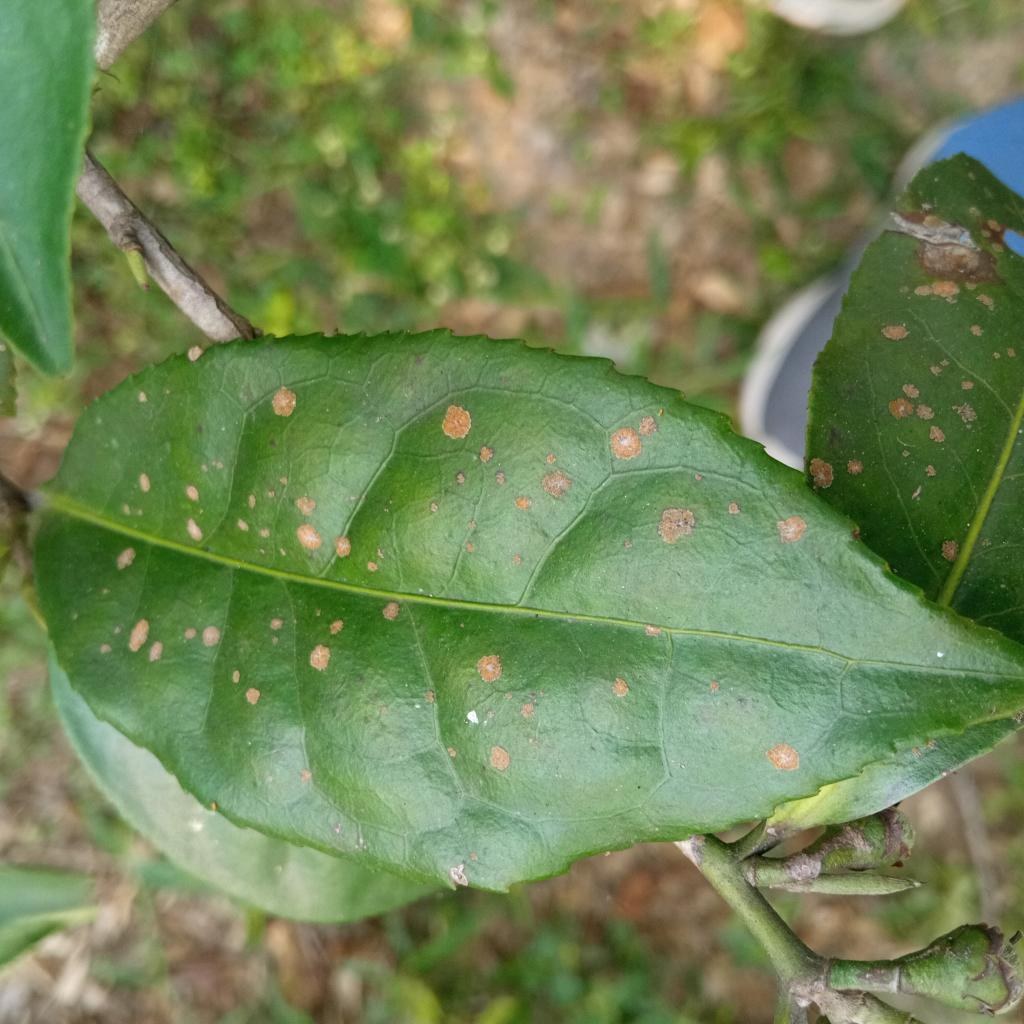
\includegraphics[width=1.62cm,height=1.00cm,keepaspectratio]
   {data_final/data_final/real_dataset_sorted/LEAF_RUST/107_jpg.rf.9c0264c78b1f4dfff87adea98349df8b.jpg}};
\node[font=\small\bfseries, anchor=south] at (0,2.24)
  {{\color{green!45!black}\faImage}~Leaf crop};
\node[chip, anchor=north] at (0,0.46) {$224\times224$};

\node[blk, text width=1.95cm, minimum height=1.70cm, fill=outyyellow]
  (text) at (0,-1.35) {};
\node[draw=black!40, fill=white, minimum width=1.62cm, align=left,
      font=\scriptsize, inner sep=3pt] at (0,-1.30)
  {scattered spots\\powdery texture\\tip affected};
\node[font=\small\bfseries, anchor=south] at (0,-0.46)
  {{\color{orange!70!black}\faStickyNote}~Field note};
\node[chip, anchor=north] at (0,-2.26) {$\leq 128$ tokens};

%============================================================ encoders
\node[blk, text width=2.60cm, minimum height=1.70cm, fill=smallgray!60]
  (vision) at (3.60,1.35)
  {{\Large\color{headblue}\faSnowflake}\,{\Large\color{black!55}\faLayerGroup}\\[2pt]
   {\small\bfseries Frozen ResNet-50}\\
   {\scriptsize\color{black!70} $49\times256$ tokens}};

\node[blk, text width=2.60cm, minimum height=1.70cm, fill=llmblue!45]
  (language) at (3.60,-1.35)
  {{\Large\color{headblue}\faFont}\,{\Large\color{black!55}\faProjectDiagram}\\[2pt]
   {\small\bfseries Text Transformer}\\
   {\scriptsize\color{black!70} 2 layers $\cdot$ 4 heads}};

%============================================================ cross-attention
\node[blk, text width=2.60cm, minimum height=3.30cm, fill=vlmred!20]
  (cross) at (7.40,0)
  {{\small\bfseries Cross-attention}\\
   {\scriptsize\color{black!70} 8 heads, both ways}\\[7pt]
   \begin{tikzpicture}[baseline=-0.6ex]
     \foreach \y in {-0.52,-0.26,0,0.26,0.52}{
       \fill[headblue]        (-0.68,\y) circle (0.085);
       \fill[orange!85!black] ( 0.68,\y) circle (0.085);
     }
     \foreach \a/\b in {-0.52/0, -0.26/0.52, 0.26/-0.26}{
       \draw[headblue, line width=0.7pt, opacity=0.9] (-0.60,\a)--(0.60,\b);
     }
     \foreach \a/\b in {0.52/-0.26, 0/0.26, -0.26/-0.52}{
       \draw[orange!85!black, line width=0.7pt, opacity=0.9] (0.60,\a)--(-0.60,\b);
     }
     \node[font=\scriptsize, text=headblue]        at (-0.68,0.86) {$H_t$};
     \node[font=\scriptsize, text=orange!75!black] at ( 0.68,0.86) {$H_v$};
   \end{tikzpicture}};

%============================================================ expert heads
\node[blk, text width=0.95cm, minimum height=0.62cm, fill=smallgray!50,
      font=\scriptsize, inner sep=3pt] (vhead) at (10.00,0.85)
  {{\color{green!40!black}\faImage}~$z_v$};
\node[blk, text width=0.95cm, minimum height=0.62cm, fill=llmblue!35,
      font=\scriptsize, inner sep=3pt] (thead) at (10.00,-0.85)
  {{\color{headblue}\faFont}~$z_t$};

%============================================================ fusion
\node[blk, text width=2.60cm, minimum height=3.30cm, fill=fedorange!60]
  (fusion) at (12.60,0)
  {{\small\bfseries Reliability fusion}\\[7pt]
   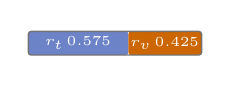
\begin{tikzpicture}[baseline=-0.6ex]
     \fill[headblue!75, rounded corners=1pt] (-1.10,-0.15) rectangle (0.17,0.15);
     \fill[orange!80!black, rounded corners=1pt] (0.17,-0.15) rectangle (1.10,0.15);
     \draw[black!55, rounded corners=1pt, line width=0.5pt]
       (-1.10,-0.15) rectangle (1.10,0.15);
     \node[font=\tiny, text=white] at (-0.47,0) {$r_t\,0.575$};
     \node[font=\tiny, text=white] at ( 0.63,0) {$r_v\,0.425$};
   \end{tikzpicture}\\[7pt]
   {\scriptsize\color{black!70} $r_t+r_v=1$}\\[2pt]
   {\scriptsize\color{black!70} $+$ residual $\lambda=2$}};

%============================================================ output
\node[blk, text width=2.70cm, minimum height=3.30cm, fill=vitgreen!30]
  (output) at (16.00,0) {};
\node[font=\small\bfseries] at (16.00,1.28)
  {{\color{green!45!black}\faChartLine}~Five-class head};
\foreach \i/\lab/\ww/\cc in {0/Blight/1.30/headblue, 1/Hoppers/0.42/black!45,
                             2/Rust/0.92/green!55!black, 3/Looper/0.64/orange!85!black,
                             4/{Mosq.}/0.34/vlmred}{
  \node[font=\tiny, anchor=east] at (15.42,0.70-0.36*\i) {\lab};
  \draw[fill=black!10, draw=none] (15.50,0.60-0.36*\i) rectangle (17.10,0.80-0.36*\i);
  \draw[fill=\cc, draw=none] (15.50,0.60-0.36*\i) rectangle (15.50+\ww,0.80-0.36*\i);
}
\node[chip, anchor=north] at (16.00,-1.02) {$p(y\mid x,t)$};

%============================================================ runtime flow
\draw[flow] (image.east)    -- (vision.west);
\draw[flow] (text.east)     -- (language.west);
\draw[flow] (vision.east)   -- (5.95,1.35);
\draw[flow] (language.east) -- (5.95,-1.35);
\draw[flow] (cross.east)    -- (fusion.west);
\draw[flow] (fusion.east)   -- (output.west);

% expert heads: branch above/below the cross block, never through it
\draw[aux] (vision.east)   -- (5.40,1.35) -- (5.40,2.08) -- (10.00,2.08)
           -- (vhead.north);
\draw[aux] (language.east) -- (5.40,-1.35) -- (5.40,-2.08) -- (10.00,-2.08)
           -- (thead.south);
\draw[aux] (vhead.east) -- ([yshift=0.85cm]fusion.west);
\draw[aux] (thead.east) -- ([yshift=-0.85cm]fusion.west);

% offline controls govern the input stage and the fused core
\draw[dashed, draw=headblue, -{Stealth[length=1.8mm]}] (0,2.95) -- (0,2.52);
\draw[dashed, draw=headblue, -{Stealth[length=1.8mm]}] (12.60,2.95) -- (12.60,1.70);

\end{tikzpicture}
}
\caption{Active inference architecture with a real corpus crop and a
representative templated note. The dashed blue boxes separate offline leakage
controls and validation-only system selection from runtime inference. The
selected ResNet--compact-Transformer core uses bidirectional cross-attention;
dashed runtime paths are explicit unimodal expert heads that re-enter the
fusion logits. The pooled ViT--DistilBERT alternative is screened separately
and is not drawn as token-level cross-attention.}
\label{fig:cross_modal_arch}
\end{figure*}
\fi
%%TRIM-END%%

\subsection{Dataset Procurement, Preparation, and Leakage Audit}
\label{sec:dataset}

\emph{Held fixed.} Every table except Table~\ref{tab:standard_suite} is scored
on the same 222/74/75 source-grouped crops, the same exact box--note pairing and
the same train-fitted leakage mask, so any difference between them is the axis
that table varies. The matched-setting
federated suite of Table~\ref{tab:standard_suite} re-partitions those same 371
observations as 260/55/56 over 199 source groups, and is read only against itself.

\textbf{Procurement and preparation.} The corpus contains 200 field photographs
from the IIT Kharagpur tea garden, supplied as JPEGs with same-stem YOLO
oriented-bounding-box (OBB) files. Each valid line records a class ID and eight
normalized corner coordinates. The loader retains each region's supplied label,
extracts its axis-aligned envelope, adds 10\% of the source width/height as
context on each side, clips to image bounds, and resizes to $224\times224$.
This yields 371 crops: leaf blight (129), leaf hoppers (9), leaf rust (67),
looper caterpillars (102), and mosquito bug (64), using raw IDs 0--4.
The acquisition rig is documented in Figure~\ref{fig:dataset_examples}f--h, but capture
dates, the handset model and sensor specification, and independent expert
adjudication are not recorded in the supplied bundle. Figure~\ref{fig:dataset_examples} shows one
real annotated crop per class; its manifest preserves source filenames,
box indices, and crop bounds. The supplied labels are not independent
confirmatory diagnoses.

\textbf{Acquisition rig.} Photographs were captured by a fixed, self-contained
station rather than handheld, which is what makes the corpus internally
consistent in scale and viewpoint. An Android handset is sealed in a weather
enclosure with a power bank (Figure~\ref{fig:dataset_examples}f--hc) and clamped to a
horizontal arm on a ground-staked pole (Figure~\ref{fig:dataset_examples}f--ha). The pole
stands $106$\,cm, the arm extends $62$\,cm over the row, and the camera sits
$11$\,cm above a mean canopy height of $95$\,cm, giving a consistent nadir view
of the plucking table (Figure~\ref{fig:dataset_examples}f--hb). Because the geometry is
fixed, apparent lesion size is comparable across photographs, and the $10\%$
context padding applied to each box corresponds to a roughly constant ground
area. The enclosure is unpowered from mains and needs no network, so the same
rig transfers to an estate without infrastructure --- the deployment assumption
the federated setting is meant to model. The rig does not record capture time,
which is why no date is available for any crop.



\begin{figure*}[t]
\centering
\begin{subfigure}[b]{0.19\textwidth}
\centering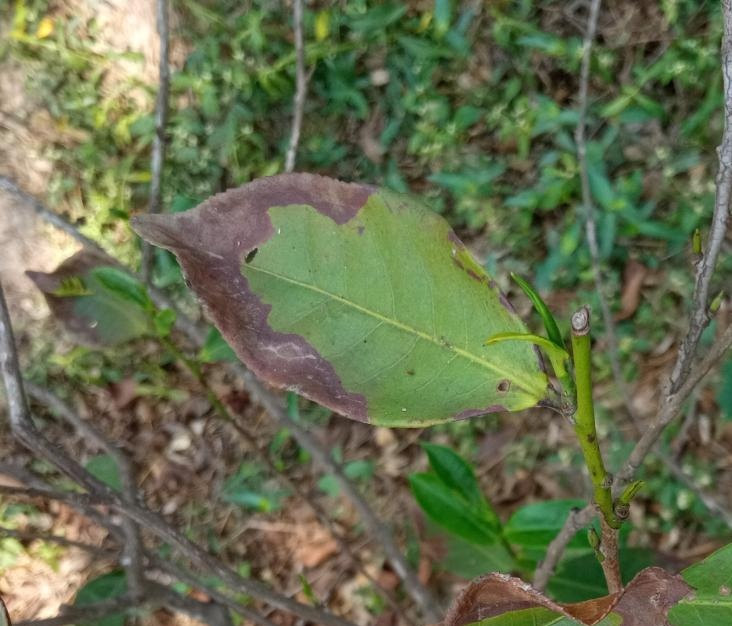
\includegraphics[width=\linewidth,height=0.85\linewidth,keepaspectratio]{dataset_examples/leaf_blight.jpg}
\caption{Leaf blight ($n=129$).}
\end{subfigure}\hfill
\begin{subfigure}[b]{0.19\textwidth}
\centering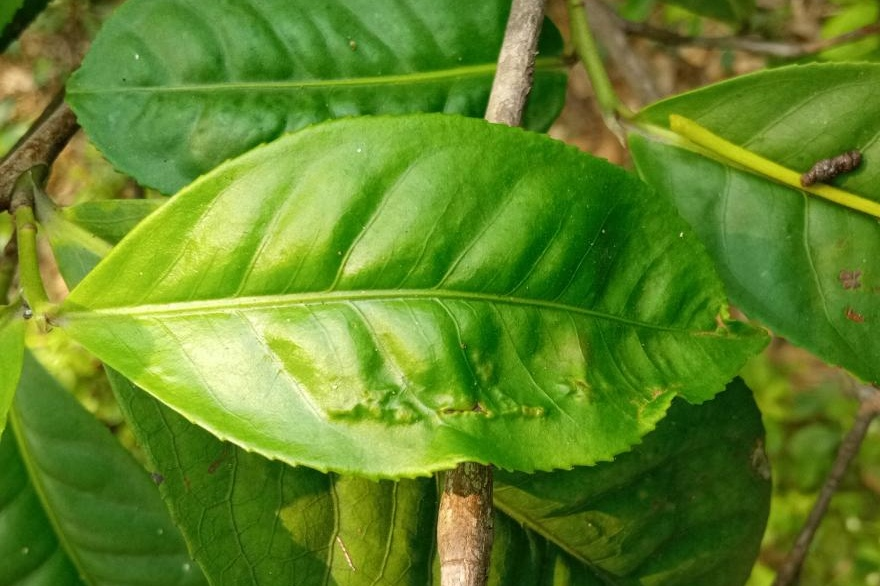
\includegraphics[width=\linewidth,height=0.85\linewidth,keepaspectratio]{dataset_examples/leaf_hoppers.jpg}
\caption{Leaf hoppers ($n=9$).}
\end{subfigure}\hfill
\begin{subfigure}[b]{0.19\textwidth}
\centering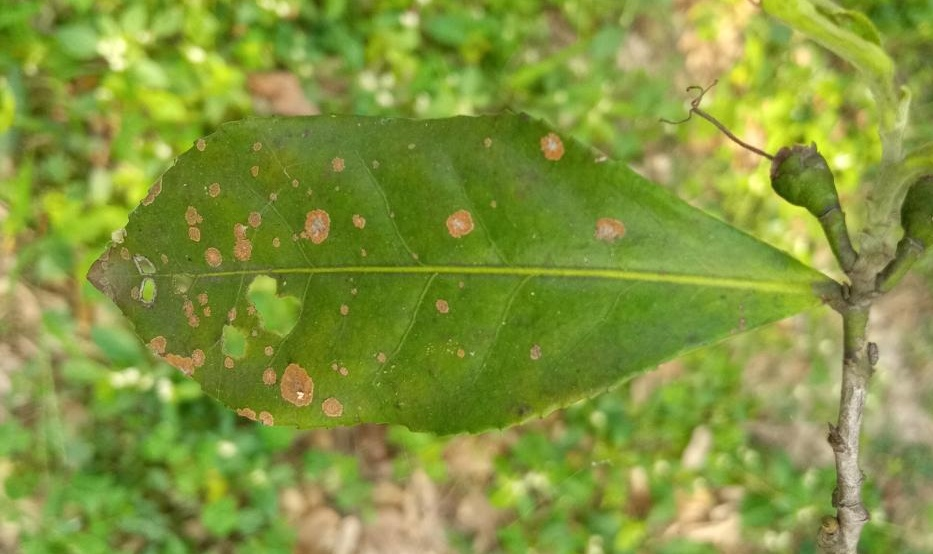
\includegraphics[width=\linewidth,height=0.85\linewidth,keepaspectratio]{dataset_examples/leaf_rust.jpg}
\caption{Leaf rust ($n=67$).}
\end{subfigure}\hfill
\begin{subfigure}[b]{0.19\textwidth}
\centering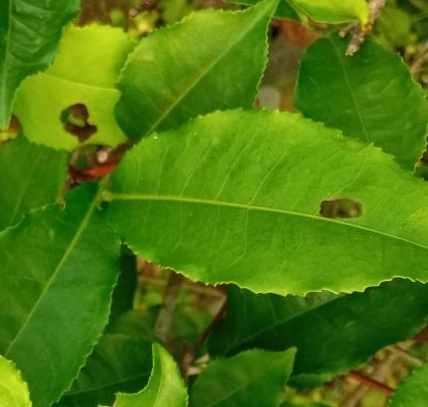
\includegraphics[width=\linewidth,height=0.85\linewidth,keepaspectratio]{dataset_examples/looper_caterpillars.jpg}
\caption{Looper ($n=102$).}
\end{subfigure}\hfill
\begin{subfigure}[b]{0.19\textwidth}
\centering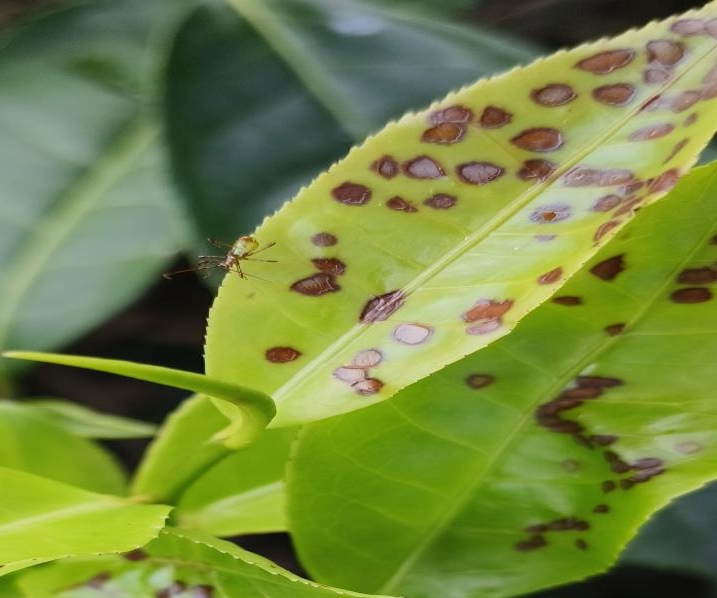
\includegraphics[width=\linewidth,height=0.85\linewidth,keepaspectratio]{dataset_examples/mosquito_bug.jpg}
\caption{Mosquito bug ($n=64$).}
\end{subfigure}

\vspace{2pt}
\begin{subfigure}[b]{0.19\textwidth}
\centering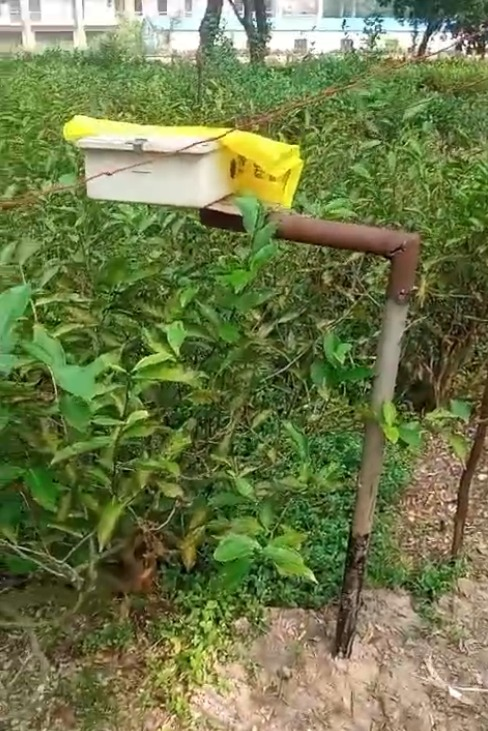
\includegraphics[width=\linewidth,height=0.85\linewidth,keepaspectratio]{setup/rig_field.jpg}
\caption{Rig in the row.}
\end{subfigure}\hfill
\begin{subfigure}[b]{0.28\textwidth}
\centering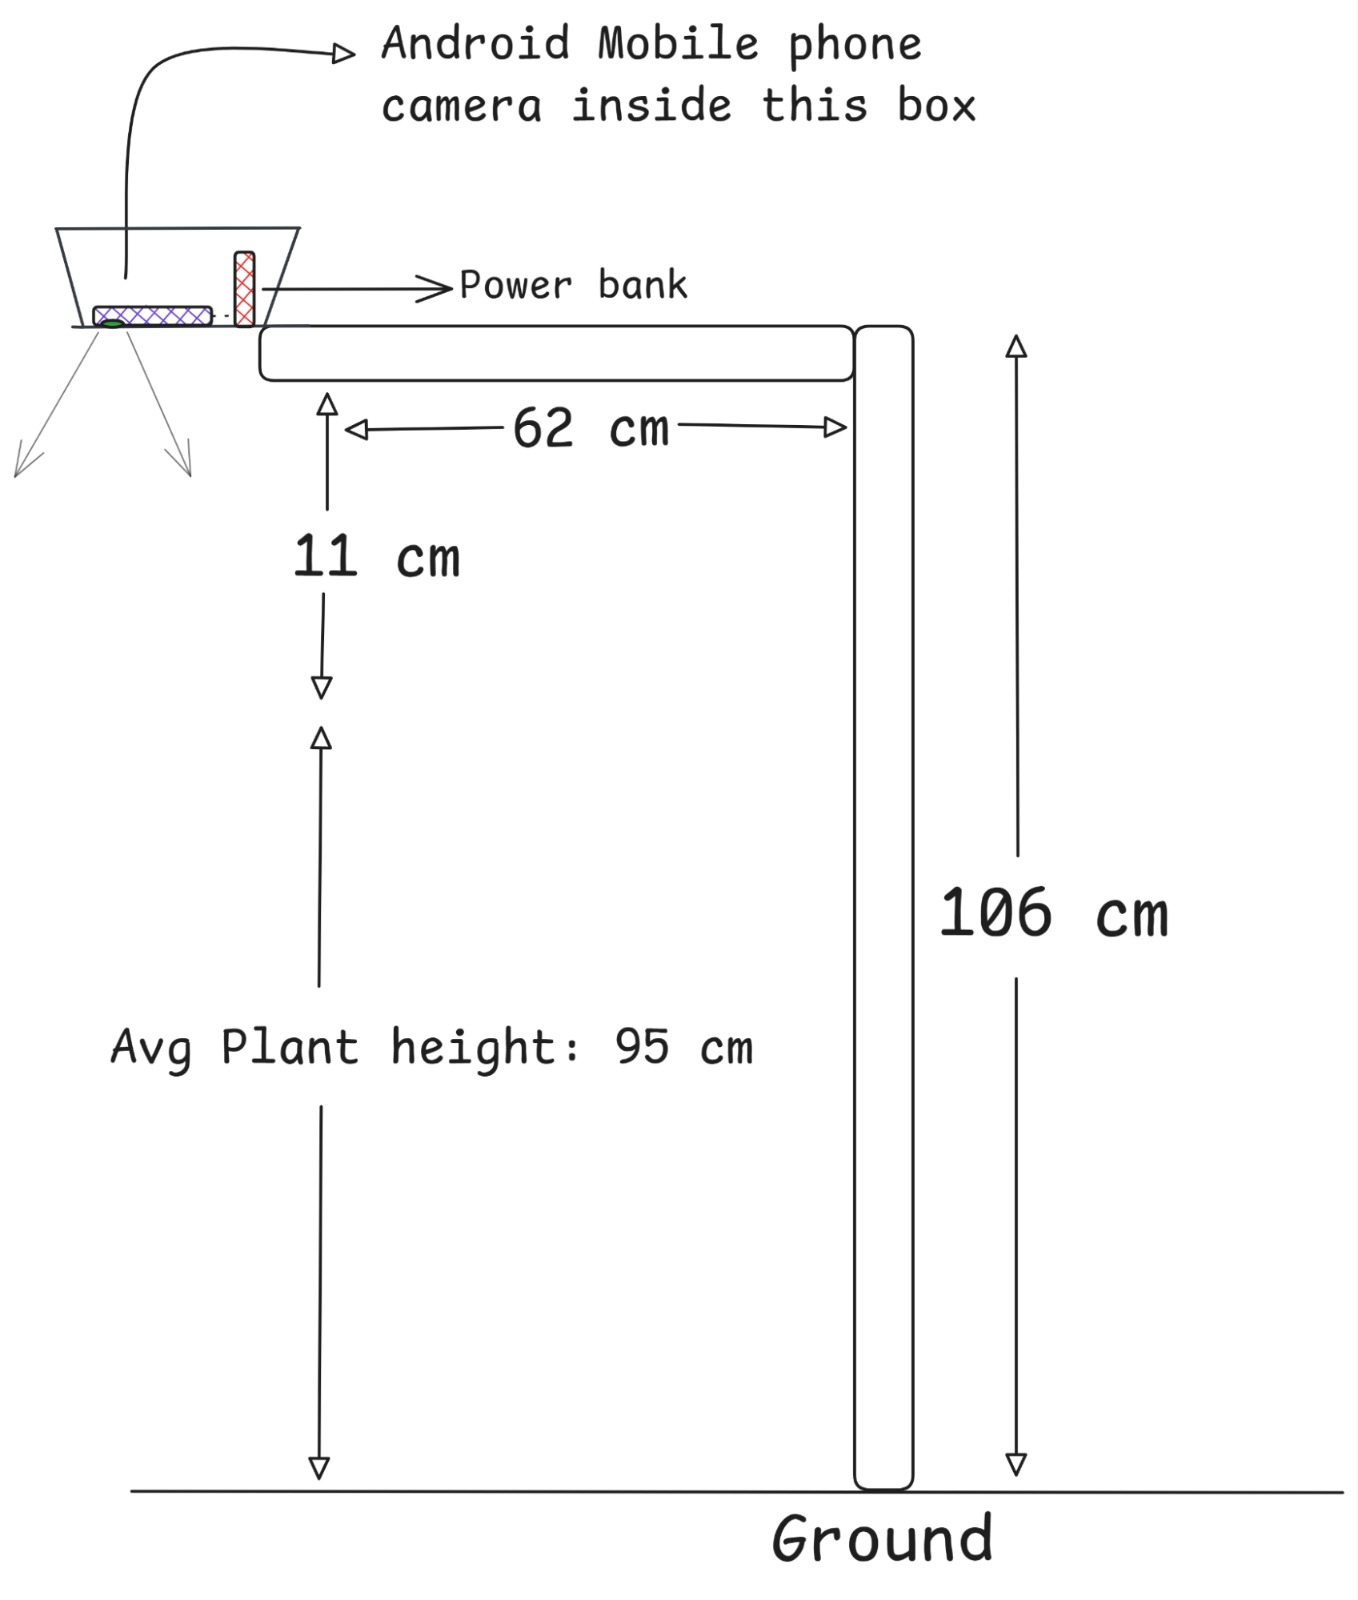
\includegraphics[width=\linewidth,height=0.85\linewidth,keepaspectratio]{setup/rig_side.jpg}
\caption{Side geometry.}
\end{subfigure}\hfill
\begin{subfigure}[b]{0.28\textwidth}
\centering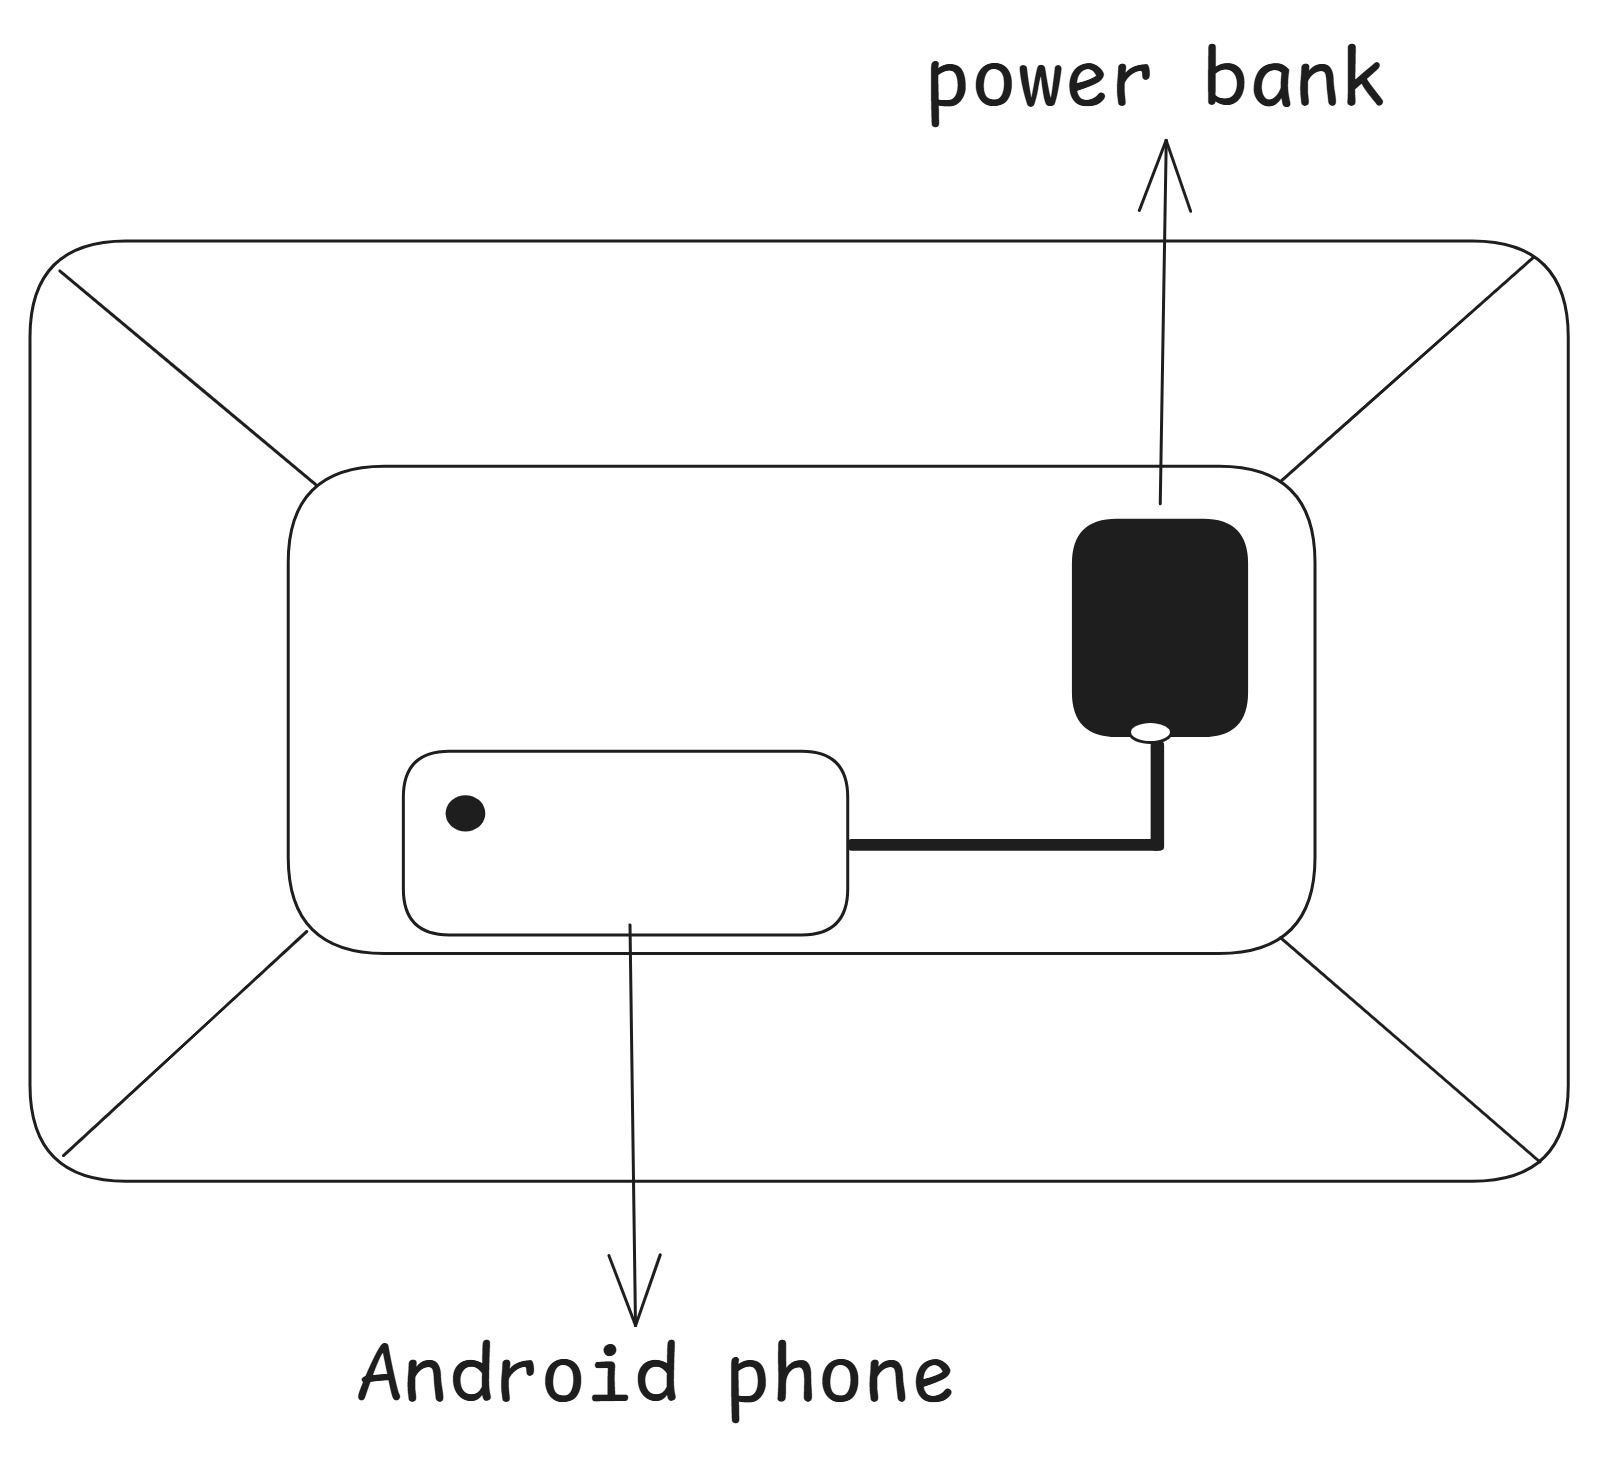
\includegraphics[width=\linewidth,height=0.85\linewidth,keepaspectratio]{setup/rig_top.jpg}
\caption{Enclosure interior.}
\end{subfigure}
\caption{Top: one actual annotated crop per class; $n$ is the corpus crop count.
Source OBB labels and 10\% context padding are preserved. Natural backgrounds and
overlapping damage patterns complicate recognition; no external or generated
images are shown. Bottom: the capture rig --- (f) deployed in the tea row, (g) a
$106$\,cm pole with a $62$\,cm arm placing the camera $11$\,cm above a $95$\,cm
mean canopy, (h) the Android handset and power bank inside the weather enclosure.
The fixed mount keeps scale and viewpoint comparable across photographs; no
capture time is logged.}
\label{fig:dataset_examples}
\end{figure*}

\begin{table}[t]
\caption{Source-grouped paired-data audit}
\label{tab:dataaudit}
\centering\footnotesize
\setlength\tabcolsep{2.8pt}
\begin{tabular}{lrrrrrr}
\toprule
\textbf{Split} & \textbf{Sources} & \textbf{Crops} & \textbf{Blight} &
\textbf{Hoppers} & \textbf{Rust} & \textbf{Looper/Mosq.}\\
\midrule
Train      & 122 & 222 & 77 & 5 & 40 & 61/39\\
Validation & 40  & 74  & 26 & 2 & 14 & 20/12\\
Test       & 38  & 75  & 26 & 2 & 13 & 21/13\\
\midrule
Total      & 200 & 371 & 129 & 9 & 67 & 102/64\\
\bottomrule
\end{tabular}
\end{table}

\textbf{Split and text provenance.} Seed 42 partitions source filenames, never
crops: overlap is zero, and test holds 75 crops from 38 unseen photographs
(Table~\ref{tab:dataaudit}). Every note links to its exact (photograph, box
index). Notes are generated from manually written phrase pools, not recorded
independently by farmers: 140 distinct sentences supply 371 notes, 61\% of
sentences occur across classes, and a class's diagnostic sign appears in 45\%
of its notes. A bag-of-words classifier reaches 0.640. The 178-token
training-derived target-pure vocabulary is frozen before evaluation.
The separate 3,000-row text bundle, augmented exports, and external studio
collections are excluded; ImageNet supplies weights only. The nine-crop
leaf-hopper class and templated language limit generalization.

\subsection{Model Variants and Objective}
\label{sec:variants}

The reliability network is a two-layer MLP over the concatenated embeddings
whose two softmax-normalized outputs give weights $r_t+r_v=1$ --- how far the
fused prediction leans on the note and on the image. An absent modality's logit
is set to $-10^{4}$ before the softmax, so its weight goes to zero and the
survivor takes the full unit of mass. The final logits are
\begin{equation}
\mathbf{z}=\mathbf{z}_f+\lambda\left(r_t\mathbf{z}_t+r_v\mathbf{z}_v\right),\qquad\lambda=2,
\label{eq:logits}
\end{equation}
where $\mathbf{z}_f$ is the fusion head's five-way output and $\mathbf{z}_t$,
$\mathbf{z}_v$ come from two linear \emph{expert} heads reading each embedding
directly. The residual weight $\lambda=2$ is
fixed rather than learned, so the two single-modality experts count twice the
fused head and a usable prediction survives when one branch is absent; a
missing modality's expert is zeroed and the residual stays active at test time.

\textbf{Comparison models.} Frozen DistilBERT~\cite{Sanh2019} and
ViT-tiny~\cite{Dosovitskiy2021} use validation-selected ridge heads. Their
late-fusion candidate uses train-fitted 64-component projections and one of 360
validation-screened linear heads; test embeddings are extracted only after the
choice is frozen. The raw and routed VLM rows are the cross-attention output
before and after the reliability router.

For one-hot label $\mathbf{y}$, training uses class-weighted, label-smoothed
cross entropy --- weights inverse to class frequency, smoothing $0.1$ --- with
auxiliary parent losses and supervised cross-modal alignment:
\begin{equation}
\mathcal{L}=\mathcal{L}_{f}
 +0.20\mathcal{L}_{t}
 +1.25\mathcal{L}_{v}
 +0.05\mathcal{L}_{align}.
\label{eq:loss}
\end{equation}
Here $\mathcal{L}_{f}$ is the loss on the fused logits; $\mathcal{L}_{t}$ and
$\mathcal{L}_{v}$ apply it to the two expert heads, averaged only over samples
where that modality is present, so a text-only batch never trains the image
expert; $\mathcal{L}_{align}$ is a supervised contrastive term over the
$\ell_2$-normalized paired embeddings, evaluated only when a batch holds at
least two paired crops. The
three weights are fixed by construction rather than tuned: image-only learning
is the harder path while templated notes make the text expert easy to satisfy,
and alignment is a regularizer that must not compete with the classification
objective. Modality dropout samples image-only, text-only and paired batches with
probabilities 0.50, 0.10, 0.40; checkpoints are selected by
$0.65F_{1,\mathrm{paired}}+0.35F_{1,\mathrm{image}}$ on validation.

For $K$ clients, the same local objective is aggregated with
FedAvg~\cite{McMahan2017},
\begin{equation}
\theta^{t+1}=\sum_{k=1}^{K}\frac{n_k}{n}\theta_k^{t+1},
\label{eq:fedobj}
\end{equation}
where $n_k$ is client $k$'s sample count. FL starts from the selected
checkpoint, freezes ResNet-50 and averages the remaining states after one
local epoch: adaptation, not training from scratch.

%% ─────────────────────────────────────────────────────────────────────────────
%%TRIM-BEGIN%% restore by deleting this line and the matching TRIM-END
\iffalse
\begin{table}[t]
\centering
\caption{Implemented model blueprint}
\label{tab:model_blueprint}
\scriptsize
\setlength{\tabcolsep}{3.2pt}
\begin{tabular}{p{0.24\columnwidth}p{0.32\columnwidth}p{0.36\columnwidth}}
\toprule
Block & Specification & Output / training state \\
\midrule
Text encoder & 192-d embedding; 2 Transformer layers; 4 heads
  & 256-d pooled vector; trainable \\
Vision encoder & ImageNet ResNet-50; $224^2$ input
  & $49{\times}256$ tokens; frozen backbone \\
Cross-attention & Two directional layers; 8 heads
  & text-to-image and image-to-text summaries \\
Reliability fusion & normalized $(r_t,r_v)$ plus interaction features
  & 5-way trainable classifier \\
Expert residual & linear text and vision heads; fixed $\lambda=2$
  & added to the fusion logits at train and test \\
Complete model & 32.20M parameters
  & 8.69M trainable parameters \\
\bottomrule
\end{tabular}
\end{table}
\fi
%%TRIM-END%%

\section{Evaluated Systems}
\label{sec:ff}

\subsection{Base Cross-Modal Checkpoint}
\label{sec:proposed}

The checkpoint trains in PyTorch for at most 15 AdamW epochs
(batch 16, peak $10^{-4}$). Two cached augmentations per training crop remain
views of 222 crops, not new samples.

% Trimmed for the page limit: the image-only inference study is not needed
% for the multimodal argument and nothing outside it references its labels.
\iffalse
\subsection{Enhanced Image-Only Inference}



Five single deployable visual systems compete on the common support, ranked by
the pre-declared validation score $0.6F_1+0.4$ accuracy, with the locked test
support reported after the choice is frozen. Across the eight visual rungs, locked
test accuracy rises from 0.613 to 0.720 (Fig.~\ref{fig:c_visual_ladder}); Figs.~\ref{fig:c_text_ladder} and~\ref{fig:c_fusion_ladder} are the corresponding text and text${+}$image ladders. \emph{Cand.} counts the configurations each rung searched, and the gate rungs route among several encoders, which is why they are marked as diagnostics.

%%TRIM-BEGIN%% restore by deleting this line and the matching TRIM-END
\iffalse
\begin{table}[t]
\centering
\caption{Single visual models on the common support, ranked by the pre-declared
validation score. \emph{Cand.} is the number of validation-fitted configurations
each system chooses among. Gates route per predicted class and are diagnostics,
not deployable single models.}
\label{tab:visual_gate}
\scriptsize
\setlength{\tabcolsep}{3.2pt}
\begin{tabular}{lrrrrr}
\toprule
\textbf{Visual system} & \textbf{Cand.} & \textbf{Val.\ acc.} & \textbf{Val.\ score} &
\textbf{Test acc.} & \textbf{Test F1}\\
\midrule
Direct ResNet path      & 1    & 0.662 & 0.644 & 0.613 & 0.543\\
Six-view TTA            & 25   & 0.730 & 0.695 & 0.613 & 0.574\\
Deep-feature head       & 40   & 0.743 & 0.698 & 0.627 & 0.540\\
Frozen ViT-tiny         & 210  & 0.797 & 0.714 & 0.667 & \textbf{0.583}\\
\rowcolor{vitgreen!40}
\textbf{Calibrated base} & 20  & 0.770 & \textbf{0.771} & \textbf{0.680} & 0.570\\
\midrule
\multicolumn{6}{l}{\emph{Per-class gates (not single models)}}\\
Three-expert gate       & 243  & 0.797 & 0.757 & 0.667 & 0.622\\
Four-expert gate        & 1024 & 0.811 & 0.783 & 0.693 & 0.653\\
Five-expert gate        & 3125 & 0.851 & 0.818 & 0.720 & 0.676\\
\bottomrule
\end{tabular}
\end{table}
\fi
%%TRIM-END%%

%% generated by experiments/make_ladder_tables.py -- do not hand-edit

%%TRIM-BEGIN%% restore by deleting this line and the matching TRIM-END
\iffalse
\begin{table}[t]
\caption{Text pipeline ladder on the common 75-crop support, with the same column structure as the visual table. \emph{Cand.} is the number of validation-fitted configurations. Each rung is repeated at three note sparsities; deletion is deterministic, so every rung sees the identical corruption of the identical notes. At complete notes a single-candidate path already reaches 0.987 accuracy and the ladder is flat, so the ceiling belongs to the corpus rather than to the pipeline. Bold marks the best single model per sparsity. This table varies the pipeline for one fixed encoder; Tables~\ref{tab:unimodal_cent_fed} and~\ref{tab:multimodal_cent_fed} vary the encoder for one fixed pipeline and add a federated column.}
\label{tab:text_ladder}
\centering\footnotesize
\setlength\tabcolsep{2.6pt}
\begin{tabular}{lrcccccc}
\toprule
& & \multicolumn{2}{c}{Complete} & \multicolumn{2}{c}{50\% deleted} & \multicolumn{2}{c}{75\% deleted}\\
\cmidrule(lr){3-4}\cmidrule(lr){5-6}\cmidrule(lr){7-8}
System & Cand. & Acc. & F1 & Acc. & F1 & Acc. & F1\\
\midrule
Direct CLS path & 1 & 0.453 & 0.360 & 0.320 & 0.263 & 0.293 & 0.192\\
Masked-mean pooling & 6 & \textbf{0.613} & 0.485 & \textbf{0.387} & 0.282 & \textbf{0.360} & 0.227\\
Last-4-layer concat & 24 & \textbf{0.613} & 0.495 & 0.360 & 0.272 & 0.293 & 0.200\\
PCA-reduced head & 30 & \textbf{0.613} & 0.501 & 0.347 & 0.249 & 0.293 & 0.197\\
\midrule
\multicolumn{8}{l}{\emph{Per-class gates (not single models)}}\\
5-expert gate & 3125 & 0.587 & 0.470 & 0.440 & 0.316 & 0.333 & 0.222\\
\bottomrule
\end{tabular}
\end{table}
\fi
%%TRIM-END%%

%%TRIM-BEGIN%% restore by deleting this line and the matching TRIM-END
\iffalse
\begin{table}[t]
\caption{Text${+}$image pipeline ladder on the same 75 crops, selected by the pre-declared validation score $0.65F_{1,\mathrm{paired}}+0.35F_{1,\mathrm{image}}$. Fusion is saturated at complete notes and separates only once notes degrade. The gate attains the best validation accuracy at 50\% deletion (0.932) yet the worst test accuracy (0.747), so its search over 243 candidates on 74 validation crops does not transfer. Bold marks the best single model per sparsity. This table varies the pipeline for one fixed encoder; Tables~\ref{tab:unimodal_cent_fed} and~\ref{tab:multimodal_cent_fed} vary the encoder for one fixed pipeline and add a federated column.}
\label{tab:mm_ladder}
\centering\footnotesize
\setlength\tabcolsep{2.6pt}
\begin{tabular}{lrcccccc}
\toprule
& & \multicolumn{2}{c}{Complete} & \multicolumn{2}{c}{50\% deleted} & \multicolumn{2}{c}{75\% deleted}\\
\cmidrule(lr){3-4}\cmidrule(lr){5-6}\cmidrule(lr){7-8}
System & Cand. & Acc. & F1 & Acc. & F1 & Acc. & F1\\
\midrule
Direct concat path & 1 & 0.667 & 0.558 & 0.613 & 0.521 & 0.560 & 0.467\\
Concat $+$ tuned head & 6 & \textbf{0.773} & 0.645 & 0.600 & 0.507 & 0.627 & 0.518\\
Deep-feature concat & 24 & \textbf{0.773} & 0.638 & 0.627 & 0.530 & 0.627 & 0.505\\
PCA-per-modality concat & 24 & 0.760 & 0.638 & 0.547 & 0.460 & 0.547 & 0.457\\
Calibrated late fusion & 9 & 0.720 & 0.592 & \textbf{0.760} & 0.637 & \textbf{0.773} & 0.642\\
\midrule
\multicolumn{8}{l}{\emph{Per-class gates (not single models)}}\\
Three-expert gate & 243 & 0.747 & 0.617 & 0.680 & 0.571 & 0.693 & 0.576\\
\bottomrule
\end{tabular}
\end{table}
\fi
%%TRIM-END%%

The same ladder runs for text and text${+}$image on the identical support, so
every rung is comparable with the others and with the visual ladder. Neither ladder is flat now that the notes no
longer determine the label. The best text rung reaches 0.613 at complete notes
and 0.360 once three quarters of the tokens are gone, while the best fusion rung
holds 0.773 at both (Fig.~\ref{fig:c_fusion_ladder}): the fused pipeline is what
survives note loss, and the validation-to-test gap still widens with search
(Fig.~\ref{fig:c_selection_gap}).

The calibrated base wins on both sides of the split on the smallest search in
the table (validation 0.771, test accuracy 0.680); the gates score higher only by
fitting more routings on 74 crops, and Fig.~\ref{fig:c_selection_gap} shows what
that costs. We carry the calibrated base as the visual path and report the gate
as a diagnostic ceiling.

%% STALE -- DO NOT RESTORE AS-IS: predates the note-leakage
%% correction (caption cites 0.853/0.653, the pre-correction ladder values); regenerate the plot
%% from current data and rewrite the caption first.
%%TRIM-BEGIN%% restore by deleting this line and the matching TRIM-END
\iffalse
\begin{figure}[t]
\centering

\includegraphics[width=0.96\linewidth]{plots/plot88_sparsity_ladder}
\caption{Every ladder rung as field notes are deleted, on the identical 75 crops; deletion is deterministic, so all rungs at a sparsity see the same corruption of the same notes. Gates are dashed and marked $*$; they are diagnostics, not deployable models. (a) Text rungs collapse from the ceiling to 0.51--0.65 once three quarters of the notes are gone. (b) Fusion rungs degrade far more gently and, at 25\% of notes retained, the best fusion rung (0.853) leads both the best text rung (0.653, dotted) and the best single visual model (0.680, dashed). This is the condition under which fusion beats both parents; at complete notes it cannot, because the text branch is already saturated.}
\label{fig:sparsity_ladder}
\end{figure}
\fi
%%TRIM-END%%

%%COMPACT-BEGIN%%
\begin{figure}[t]
\centering

\includegraphics[width=\figw]{plots/c01_text_ladder}
\caption{Text-only accuracy on 75 crops under note deletion; the best rung falls from 0.613 to 0.360. Dashed gates ($*$) are diagnostic.}
\label{fig:c_text_ladder}
\end{figure}
%%COMPACT-END%%

%%COMPACT-BEGIN%%
\begin{figure}[t]
\centering

\includegraphics[width=\figw]{plots/c02_fusion_ladder}
\caption{Fusion under the same deletion: the best rung retains at least 0.760 while text-only falls to 0.360.}
\label{fig:c_fusion_ladder}
\end{figure}
%%COMPACT-END%%

%%COMPACT-BEGIN%%
\begin{figure}[t]
\centering

\includegraphics[width=\figw]{plots/c03_visual_search}
\caption{Alternative image-only systems and search budgets. Accuracy rises from 0.613 to 0.720; hatched class-specific gates are diagnostic, not deployable models.}
\label{fig:c_visual_ladder}
\end{figure}
%%COMPACT-END%%

\fi

\subsection{Reliability-Aware Sparse-Note Rule}

For sparse notes, a stable hash retains each non-special token with probability
0.50. A validation-fixed rule routes low-confidence ($<0.60$), base-predicted
leaf-rust cases to the sparse-text expert; otherwise it keeps late fusion. Because
the routing family was refined on this internal partition, its test score is
\textbf{exploratory and non-pristine}.

%%TRIM-BEGIN%% restore by deleting this line and the matching TRIM-END
\iffalse
\begin{figure*}[t]
\centering
\resizebox{0.8718\textwidth}{!}{% Deterministic sparse-note router -- pictorial version. Validation controls stay
% visibly separated from the frozen test-time decision path.
% Requires fontawesome5 and TikZ libraries arrows.meta, positioning, shapes.geometric.
\begin{tikzpicture}[
  font=\small,
  >={Stealth[length=2.4mm,width=1.8mm]},
  flow/.style={->, thick, draw=black!70},
  selected/.style={->, very thick, draw=headblue},
  route/.style={draw=black!45, rounded corners=4pt, thick, fill=white,
                minimum width=3.75cm, minimum height=1.05cm, align=center,
                inner xsep=5pt, inner ysep=3pt},
  chip/.style={draw=black!32, rounded corners=3pt, fill=white,
               inner xsep=4pt, inner ysep=2pt, font=\scriptsize, align=center},
  decision/.style={diamond, aspect=2.0, draw=black!60, line width=1pt,
                   fill=outyyellow, align=center, inner xsep=1pt, inner ysep=1pt,
                   font=\scriptsize\bfseries},
  outcome/.style={draw=headblue, rounded corners=4pt, line width=1pt, fill=blue!4,
                  minimum width=3.60cm, minimum height=1.85cm, align=center}
]

%------------------------------------------------- validation-only rule strip
\node[draw=headblue, dashed, rounded corners=4pt, fill=blue!3,
      minimum width=15.0cm, minimum height=0.74cm] (validation) at (7.90,2.95) {};
\node[anchor=west, font=\scriptsize] at ([xshift=6pt]validation.west)
  {{\color{headblue}\faSlidersH}~\textbf{Rule fitted on validation only:}};
\node[chip, anchor=west, fill=green!5] at ([xshift=4.55cm]validation.west)
  {\faImage~image gate for hopper / bug};
\node[chip, anchor=west, fill=blue!5] at ([xshift=8.30cm]validation.west)
  {\faFont~sparse text if rust \& $p_{\max}<0.60$};
\node[chip, anchor=west, fill=black!5] at ([xshift=12.55cm]validation.west)
  {\faLock~then frozen};

%------------------------------------------------- candidate routes
\node[route, fill=green!8] (image) at (2.05,1.45)
  {{\large\color{green!45!black}\faImage}~\textbf{Enhanced image}\\
   {\scriptsize\color{black!65} five-expert class gate}};
\node[route, fill=llmblue!30] (text) at (2.05,0.15)
  {{\large\color{headblue}\faFont}~\textbf{Sparse text}\\
   {\scriptsize\color{black!65} 50\% token retention}};
\node[route, fill=fedorange!55] (late) at (2.05,-1.15)
  {{\large\color{orange!75!black}\faLayerGroup}~\textbf{Late fusion}\\
   {\scriptsize\color{black!65} paired score $+$ image gate}};
\node[route, fill=vlmred!25] (raw) at (2.05,-2.45)
  {{\large\color{vlmred!70!black}\faBrain}~\textbf{Raw cross-modal}\\
   {\scriptsize\color{black!65} base paired checkpoint}};

\foreach \n/\c in {image/green!55!black, text/headblue, late/orange!85!black,
                   raw/vlmred}{
  \draw[\c, line width=3pt]
    ([xshift=0.09cm,yshift=0.26cm]\n.south west) --
    ([xshift=0.09cm,yshift=-0.26cm]\n.north west);
}

%------------------------------------------------- fan-in bus
\node[draw=black!45, rounded corners=3pt, thick, fill=black!5,
      minimum width=0.50cm, minimum height=4.55cm] (pool) at (5.10,-0.50) {};
\node[font=\scriptsize, rotate=90, text=black!60] at (5.10,-0.50)
  {four candidate routes};

%------------------------------------------------- decisions
\node[decision] (imageclass) at (8.10,0.35)
  {base class\\ hopper / bug?};
\node[decision] (lowconf) at (11.75,0.35)
  {rust \&\\ $p_{\max}{<}0.60$?};

%------------------------------------------------- outcomes
\node[chip, fill=green!8, draw=green!45!black, minimum height=0.55cm]
  (useimage) at (8.10,-1.75) {{\color{green!45!black}\faImage}~image route};
\node[chip, fill=llmblue!30, draw=headblue, minimum height=0.55cm]
  (usetext) at (11.75,-1.75) {{\color{headblue}\faFont}~sparse-text route};
\node[chip, fill=fedorange!55, draw=orange!70!black, minimum height=0.55cm]
  (uselate) at (15.40,-1.75) {{\color{orange!75!black}\faLayerGroup}~keep late / raw};

%------------------------------------------------- final probability vector
\node[outcome] (output) at (19.05,-1.10) {};
\node[font=\small\bfseries, anchor=north] at ([yshift=-0.08cm]output.north)
  {{\color{headblue}\faChartLine}~Five-class output};
\foreach \i/\lab/\ww/\cc in {0/Blight/1.10/headblue, 1/Hoppers/0.30/black!45,
                             2/Rust/0.78/green!55!black, 3/Looper/0.50/orange!85!black,
                             4/{Mosq.}/0.26/vlmred}{
  \node[font=\tiny, anchor=east] at (18.30,-0.72-0.24*\i) {\lab};
  \draw[fill=black!10, draw=none] (18.36,-0.79-0.24*\i) rectangle (19.70,-0.65-0.24*\i);
  \draw[fill=\cc, draw=none] (18.36,-0.79-0.24*\i) rectangle (18.36+\ww,-0.65-0.24*\i);
}
\node[chip, fill=green!4, draw=green!45!black] at (19.05,0.35)
  {\faLock~frozen before test inference};

%------------------------------------------------- wiring
\foreach \n in {image,text,late,raw}{
  \draw[flow] (\n.east) -- (pool.west |- \n.east);
}
\draw[flow] (pool.east) -- ++(0.30,0) |- (imageclass.west);

\draw[selected] (imageclass.east) -- node[above,font=\scriptsize,text=black!60]{no}
  (lowconf.west);
\draw[selected] (imageclass.south) -- node[right,font=\scriptsize]{yes} (useimage.north);
\draw[selected] (lowconf.south) -- node[right,font=\scriptsize]{yes} (usetext.north);
\draw[selected] (lowconf.east) -- ++(0.45,0)
  |- node[pos=0.72,above,font=\scriptsize]{no} (uselate.west);

\draw[flow] (useimage.south) -- ++(0,-0.80) -| (output.south);
\draw[flow] (usetext.south)  -- ++(0,-0.80) -| (output.south);
\draw[flow] (uselate.east) -- (output.west |- uselate.east);

\draw[dashed,draw=headblue,-{Stealth[length=1.8mm]}]
  (validation.south) -- (imageclass.north);

\end{tikzpicture}
}
\caption{Reliability-aware sparse-note routing as an explicit decision flow.
Four available prediction routes feed a deterministic class/confidence rule
selected on validation. Blue arrows show the frozen decisions; the router does
not read test labels, and the reported internal result remains exploratory and
non-pristine.}
\label{fig:reliability_router}
\end{figure*}
\fi
%%TRIM-END%%


%%COMPACT-BEGIN%%
\begin{figure}[t]
\centering

\includegraphics[width=\figw]{plots/c04_selection_gap}
\caption{Validation minus test accuracy per system on the aligned support. A large positive gap is selection that did not transfer from 74 validation crops.}
\label{fig:c_selection_gap}
\end{figure}
%%COMPACT-END%%

\subsection{Multimodal Federated Adaptation}

FL adapts 8.69M parameters with frozen ResNet-50, one local epoch, full
participation, and sample weighting. We sweep $K=\{2,3,5,8\}$ for eight rounds
over seeds 42, 123, and 2026 on the 74-crop validation set. Clients are simulated;
the ensemble and router are excluded from this FL score.

The two halves of a round separate cleanly: every stage
touching a photograph, box, or note runs on the client.

%%TRIM-BEGIN%% restore by deleting this line and the matching TRIM-END

\begin{figure*}[tbp]
\centering
\resizebox{0.8363\textwidth}{!}{% Edge/cloud division of labour in one FedAvg round -- pictorial version.
% REQUIRES: TikZ libraries arrows.meta, positioning, fit, shapes.geometric,
%           shapes.symbols; package fontawesome5. Colours from the main preamble.
%
% Layout note: the client panel is kept narrow enough (tiles 3.42cm text width,
% 3.771cm pitch) and the cloud pushed far enough right that the "weights only"
% callout sits entirely in the gap between the trainable core and the cloud.
% Keep >= 0.3cm clearance on both sides of that badge when editing.
\begin{tikzpicture}[
  font=\normalsize,
  >={Stealth[length=3.4mm,width=2.6mm]},
  tile/.style={draw=black!45, rounded corners=5pt, very thick, align=center,
               inner sep=3pt, text width=3.42cm, minimum height=2.15cm, fill=white},
  badge/.style={draw=black!35, rounded corners=3pt, fill=white, font=\small,
                inner xsep=4pt, inner ysep=2pt, align=center},
  hdr/.style={font=\small\bfseries, draw=black!45, rounded corners=4pt,
              inner xsep=5pt, inner ysep=2.5pt},
  stepbadge/.style={circle, fill=black!80, text=white, minimum size=5.8mm,
                    inner sep=0pt, font=\small\bfseries},
  flow/.style={->, very thick, draw=black!60},
  upl/.style={->, ultra thick, draw=orange!85!black, rounded corners=6pt},
  dnl/.style={->, ultra thick, dashed, draw=headblue, rounded corners=6pt}
]

%---------------------------------------------------------------- client stack
\draw[rounded corners=8pt, draw=black!25, fill=black!4, very thick]
  (0.55,-0.05) rectangle (16.15,4.05);
\draw[rounded corners=8pt, draw=black!30, fill=black!7, very thick]
  (0.30,0.10) rectangle (15.90,4.20);

%---------------------------------------------------------------- edge device
\node[draw=black!55, rounded corners=8pt, line width=1.1pt, fill=vitgreen!12,
      minimum width=15.60cm, minimum height=4.30cm] (dev) at (7.80,2.20) {};

\node[tile, fill=vitgreen!45] (t1) at (2.24,2.72)
  {{\huge\color{green!45!black}\faLeaf}\,{\huge\color{black!55}\faStickyNote}\\[1pt]
   {\small\bfseries Linked record}\\
   {\scriptsize\color{black!70} leaf photo $+$ its own note}};

\node[tile, fill=vitgreen!45] (t2) at (6.01,2.72)
  {{\huge\color{black!55}\faCrop}\,{\huge\color{black!55}\faFilter}\\[1pt]
   {\small\bfseries Crop \& mask}\\
   {\scriptsize\color{black!70} $224^2$ $\cdot$ 178-token filter}};

\node[tile, fill=smallgray!70] (t3) at (9.78,2.72)
  {{\huge\color{headblue}\faSnowflake}\,{\huge\color{black!55}\faLayerGroup}\\[1pt]
   {\small\bfseries Frozen ResNet-50}\\
   {\scriptsize\color{black!70} 23.5\,M $\cdot$ no gradients}};

\node[tile, fill=fedorange!80] (t4) at (13.55,2.72)
  {{\huge\color{vlmred!70!black}\faBrain}\,{\huge\color{black!55}\faCogs}\\[1pt]
   {\small\bfseries Trainable core}\\
   {\scriptsize\color{black!70} 8.69\,M $\cdot$ one local epoch}};

\draw[flow] (t1) -- (t2);
\draw[flow] (t2) -- (t3);
\draw[flow] (t3) -- (t4);

%---- data-locality strip inside the device
\node[badge, fill=green!8, draw=green!45!black, minimum width=14.30cm,
      minimum height=0.58cm] at (7.80,0.85)
  {{\color{green!35!black}\faLock}~\textbf{photos $\cdot$ notes $\cdot$ boxes never leave the device}};

\node[hdr, fill=vitgreen!60, anchor=west] at (0.55,4.20)
  {\faMobile~(a) Edge device --- client $k$};
\node[badge, anchor=east] at (15.05,4.20)
  {\faSitemap~$\times\,K$ clients ($K=2,3,5,8$)};

%---------------------------------------------------------------- boundary
\draw[densely dotted, black!55, line width=1.1pt] (17.40,-0.45) -- (17.40,4.55);
\node[fill=white, inner sep=2pt, text=black!65, font=\small\bfseries]
  at (17.40,4.72) {\faUserShield~privacy boundary};

%---------------------------------------------------------------- cloud
\node[cloud, draw=headblue, line width=1.1pt, fill=llmblue!45, aspect=2.0,
      cloud puffs=13, cloud puff arc=115, minimum width=7.4cm,
      minimum height=3.55cm, align=center] (cl) at (23.10,2.30)
  {{\LARGE\color{headblue}\faServer}\\[-2pt]
   {\small\bfseries FedAvg}\\[1pt]
   $\displaystyle\theta^{t+1}=\sum_{k=1}^{K}\frac{n_k}{n}\,\theta_k^{t+1}$\\[1pt]
   {\scriptsize\color{black!70} $T=8$ rounds $\cdot$ warm start}};

\node[hdr, fill=llmblue!70, anchor=west] at (19.55,4.52)
  {\faCloud~(b) Cloud --- coordination only};

\node[badge, fill=vlmred!20, draw=vlmred!80] at (23.10,0.05)
  {{\color{vlmred!60!black}\faBan}~\textbf{no raw data received}};

%---------------------------------------------------------------- traffic
\draw[upl] (t4.east) -- (19.95,2.72);
\node[badge, fill=orange!10, draw=orange!70!black, anchor=south]
  at (17.40,2.98) {{\color{orange!70!black}\faUpload}~\textbf{weights only:} $\theta_k^{t+1}$};

\draw[dnl] (cl.-35) |- (16.15,-0.90) -| (t4.south);
\node[badge, fill=blue!5, draw=headblue, anchor=south]
  at (11.80,-0.78) {{\color{headblue}\faSatelliteDish}~broadcast $\theta^{t+1}$};

\node[stepbadge] at (0.82,3.52) {1};
\node[stepbadge] at (12.02,3.52) {2};
\node[stepbadge] at (20.35,2.20) {3};
\node[stepbadge] at (21.05,3.20) {4};
\node[stepbadge] at (15.60,-0.90) {5};

\end{tikzpicture}
}
\caption{One FedAvg round: box-linked loading, cropping, masking, and local training of 8.69M parameters remain on the client. The server averages updates; fusion uplink costs 59.5--60.5\,MiB per client-round.}
\label{fig:edge_cloud}
\end{figure*}

%%TRIM-END%%


\subsection{Advisory Module}
\label{sec:rag}

The Classify--Retrieve--Advise module embeds a query with
Sentence-BERT~\cite{Reimers2019} and performs exact FAISS inner-product
search. Its corpus is textual only and shares no
records with the box-linked crop set: 673 unique observations (132--138 per class)
built from 131 distinct templated sentences. A deduplicated split leaves 472
passages and 201 queries with no shared observation. Correctness requires a class
match.

\section{FarmFederate Application and Practical Use}
\label{sec:app}

FarmFederate is the Flutter advisory prototype associated with LEAF.
Figure~\ref{fig:app_screens} shows its six screens. Sign-in leads to a
dashboard (a) with crop-check/chat shortcuts, service status, and sensor cards.
``Check My Crops'' (b) accepts a camera or gallery photograph, a plain-language
symptom description, or both; example prompts and optional sensor context
support entry, and analysis settings expose text, image, and fusion choices.
Results (c) present a status, category scores, and recommended actions, while
AI chat (d) supports follow-up questions with text and image input. Analytics
(e) and farm-network (f) screens present trend and round/participant views.

\textbf{Practical value.} A scout can photograph a suspect leaf, describe its
progression, inspect feedback, and ask for clarification in one interface,
which organizes field evidence into a shared starting point for
extension-worker review; readable results and conversation help growers
interpret model outputs, and monitoring views give supervisors context. These
are intended workflow benefits: time savings, adoption, yield gains, and
reduced input use were not measured.

\textbf{Prototype scope.} Screenshot scores and broad stress labels such as
``Needs Water'' are demonstration content, distinct from the five-class tea
results. Analytics history is simulated and farm-network state is preset, so
these screens do not establish live telemetry or multi-estate FL; sensor input
is not a third evaluated modality. The client sends images and notes to a
configured inference backend, so the FL training boundary does not imply
on-device inference. Deployment requires the selected tea checkpoint, its
exact label schema, measured services, and field validation.

\begin{figure*}[t]
\centering
%% Six prototype screenshots, each framed in a drawn phone outline.
%% \phoneshot is defined in the main.tex preamble; screenshots are unmodified
%% files from plots/app/ and are only clipped to the rounded screen area.
\newcommand{\phonecell}[2]{%
\begin{subfigure}[b]{0.158\textwidth}
\centering\phoneshot{app/#1}%
\caption{#2}
\end{subfigure}}
\phonecell{home.jpeg}{Dashboard}\hfill
\phonecell{cropcheck_input.jpeg}{Crop check}\hfill
\phonecell{cropcheck_results.jpeg}{Results}\hfill
\phonecell{aichat.jpeg}{AI chat}\hfill
\phonecell{analytics.jpeg}{Analytics}\hfill
\phonecell{farm_network.jpeg}{Farm network}

\caption{FarmFederate prototype screens in drawn phone outlines; screenshots
are unmodified. Displayed scores, sensor values, and broad stress labels are
demonstration content, and (e)--(f) show simulated history and preset network
state, not audited LEAF results.}
\label{fig:app_screens}
\end{figure*}

%% ─────────────────────────────────────────────────────────────────────────────

\section{Performance Evaluation}
\label{sec:eval}

\subsection{Protocol}

All crops from a source photograph remain in one partition. Model selection and
the five-expert visual gate use only the 74-crop validation partition; every
number below uses the same 75-crop, 38-source internal test support. Macro F1
accompanies accuracy because the classes are imbalanced. Source-group bootstrap
intervals (5,000 replicates) resample source photographs rather than crops.

Five evidence tracks remain separate: the exact-pair same-checkpoint ablation;
the validation-selected family comparison on the common 75-crop support; the
74-crop validation-only FedAvg sweep; earlier text, vision, and proxy-fusion
screens whose differing supports permit only within-panel ranking; and the
371-pair matched-setting suite on genuine box-linked observations, with no
label-matched resampling and no synthetic images.

\subsection{Federated Client and Round Scaling}

%%TRIM-BEGIN%% restore by deleting this line and the matching TRIM-END
\iffalse
\begin{table}[t]
\centering
\caption{Validation-only multimodal FedAvg adaptation. Values are
means over three client-partition seeds.}
\label{tab:fl_adaptation}
\scriptsize
\setlength{\tabcolsep}{2.1pt}
\begin{tabular}{rrrrr}
\toprule
$K$ & Final F1 & Best F1 & Retained & Label TV \\
\midrule
2 & 0.8924 & 0.9099 & 98.1\% & 0.139 \\
3 & 0.9046 & 0.9237 & 99.4\% & 0.217 \\
5 & 0.9099 & 0.9297 & 100.0\% & 0.270 \\
8 & 0.9099 & 0.9099 & 100.0\% & 0.300 \\
\bottomrule
\end{tabular}
\end{table}
\fi
%%TRIM-END%%


%%COMPACT-BEGIN%%
\begin{figure}[t]
\centering

\includegraphics[width=\figw]{plots/c22_core_rounds}
\caption{Rounds against performance for the retained core, one line per client
count. Dashed: the centralized initialization each run adapts from. $K{=}2$ and
3 climb toward it; $K{=}5$ and 8 are flat.}
\label{fig:c_core_rounds}
\end{figure}
%%COMPACT-END%%

%%COMPACT-BEGIN%%
\begin{figure}[t]
\centering

\includegraphics[width=\figw]{plots/c23_core_clients}
\caption{Clients against performance for the retained core: the same fixed
training set split over more owners. Bars are $\pm$1 SD over 3 seeds; realized
label TV is printed under each tick.}
\label{fig:c_core_clients}
\end{figure}
%%COMPACT-END%%

Figs.~\ref{fig:c_core_rounds} and~\ref{fig:c_core_clients} answer the two
federated scaling questions directly. Final-round macro F1 falls from 0.6527 at
$K=2$ to 0.5846 at $K=8$ against a centralized initialization of 0.6919, so
84--94\% is retained: adaptation costs something on the corrected corpus where
it cost almost nothing on the saturated one. Round-wise means stay between 0.5735 and 0.6857, the
highest a $K=3$ transient at round 7 rather than the final model. Realized
label-distribution total variation rises with $K$ from 0.151 to 0.281 without a
monotone final-score penalty, over 3 partition seeds.

This result is narrow: every run begins from the same centrally selected
checkpoint, so it supports federated adaptation of the multimodal core, not
superiority over training from scratch. Three partition seeds measure
ownership-split variability, not checkpoint-training variance, and simulated
clients cannot establish estate-level privacy.

\subsection{Matched-Setting Controlled Ablations}

%%TRIM-BEGIN%% restore by deleting this line and the matching TRIM-END
\iffalse
\begin{figure*}[t]
\centering
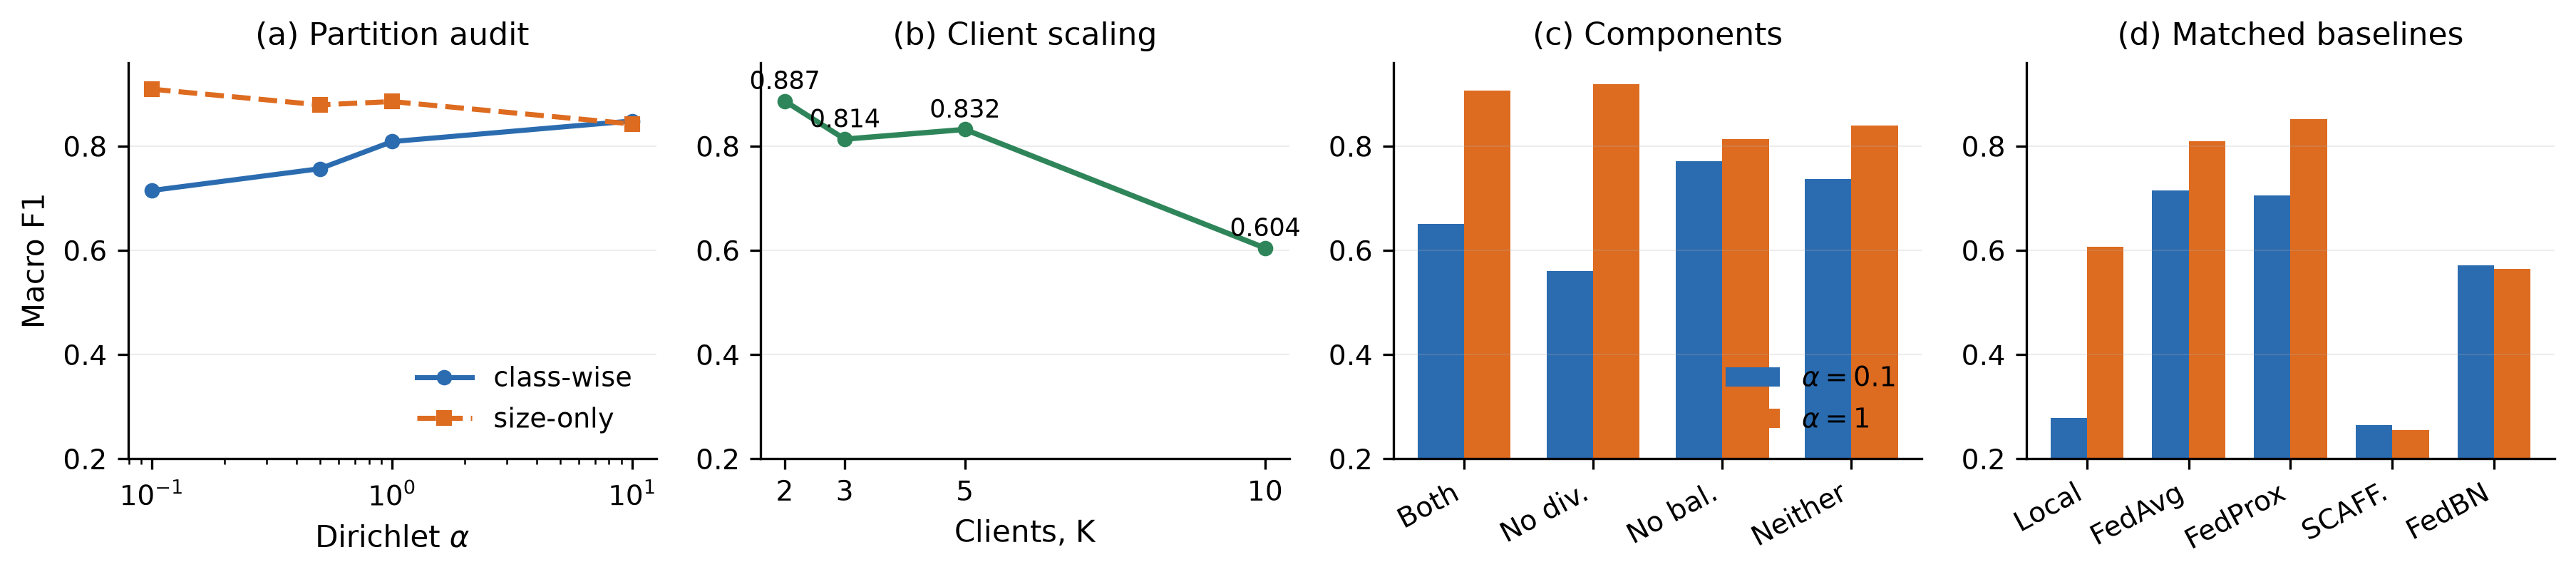
\includegraphics[width=0.7482\textwidth]{plots/plot79_standard_suite}
\caption{Standard-tier controlled suite. (a) The class-wise Dirichlet splitter
creates the intended label skew; the legacy size-only splitter does not.
(b) With fixed total data, $K=10$ leaves much smaller client shards.
(c) Anti-collapse components are ablated under actual federation.
(d) Aggregators use the same backbone, partition, optimizer, and local budget.
Bars in (c)--(d) compare $\alpha=0.1$ and 1; E1/E8 average seeds 0 and 1,
whereas E2/E3 use seed 0.}
\label{fig:standard_suite}
\end{figure*}
\fi
%%TRIM-END%%


%% generated by experiments/make_standard_suite_table.py -- do not hand-edit

\begin{table*}[t]
\caption{Matched federated suite: 371 box-linked crops, 260/55/56 split over 199 source groups, no synthetic images. Architectures share client partitions; entries are three-seed validation macro-F1 means over 50 rounds.}
\label{tab:standard_suite}
\centering\scriptsize
\setlength\tabcolsep{2.7pt}
\begin{minipage}[t]{0.38\textwidth}
\centering
\textbf{(a) FedAvg by architecture and skew}
\begin{tabular}{lcccc}
\toprule
Architecture & $\alpha{=}.1$ & $\alpha{=}.5$ & $\alpha{=}1$ & $\alpha{=}10$\\
\midrule
Image only        & 0.513 & 0.516 & 0.479 & 0.486\\
Text only         & 0.468 & 0.448 & 0.441 & 0.431\\
Concat VLM        & 0.531 & 0.551 & 0.548 & 0.546\\
Attention VLM     & 0.541 & 0.555 & 0.524 & 0.561\\
Cross-attn.\ VLM  & 0.499 & 0.485 & 0.466 & 0.512\\
\bottomrule
\end{tabular}
\end{minipage}\hfill
\begin{minipage}[t]{0.30\textwidth}
\centering
\textbf{(b) Aggregator at $\alpha{=}0.1$}
\begin{tabular}{lcccc}
\toprule
Arch. & Avg & Prox & SCAF & BN\\
\midrule
Image      & \textbf{.513} & .504 & .222 & .196\\
Text       & .468 & .467 & .220 & \textbf{.470}\\
Concat     & .531 & \textbf{.560} & .179 & .427\\
Attention  & .541 & \textbf{.549} & .130 & .427\\
Cross-att  & \textbf{.499} & .482 & .294 & .455\\
\bottomrule
\end{tabular}
\end{minipage}\hfill
\begin{minipage}[t]{0.28\textwidth}
\centering
\textbf{(c) Cost and federation gain}
\begin{tabular}{lcc}
\toprule
Architecture & MiB & $\Delta$ local\\
\midrule
Image only        & 18.9 & $+$0.215\\
Text only         & 42.4 & $+$0.124\\
Concat VLM        & 59.5 & $+$0.229\\
Attention VLM     & 60.5 & $+$0.219\\
Cross-attn.\ VLM  & 67.2 & $+$0.138\\
\bottomrule
\end{tabular}
\end{minipage}
\end{table*}

%%TRIM-BEGIN%% restore by deleting this line and the matching TRIM-END
\iffalse
\begin{figure*}[t]
\centering
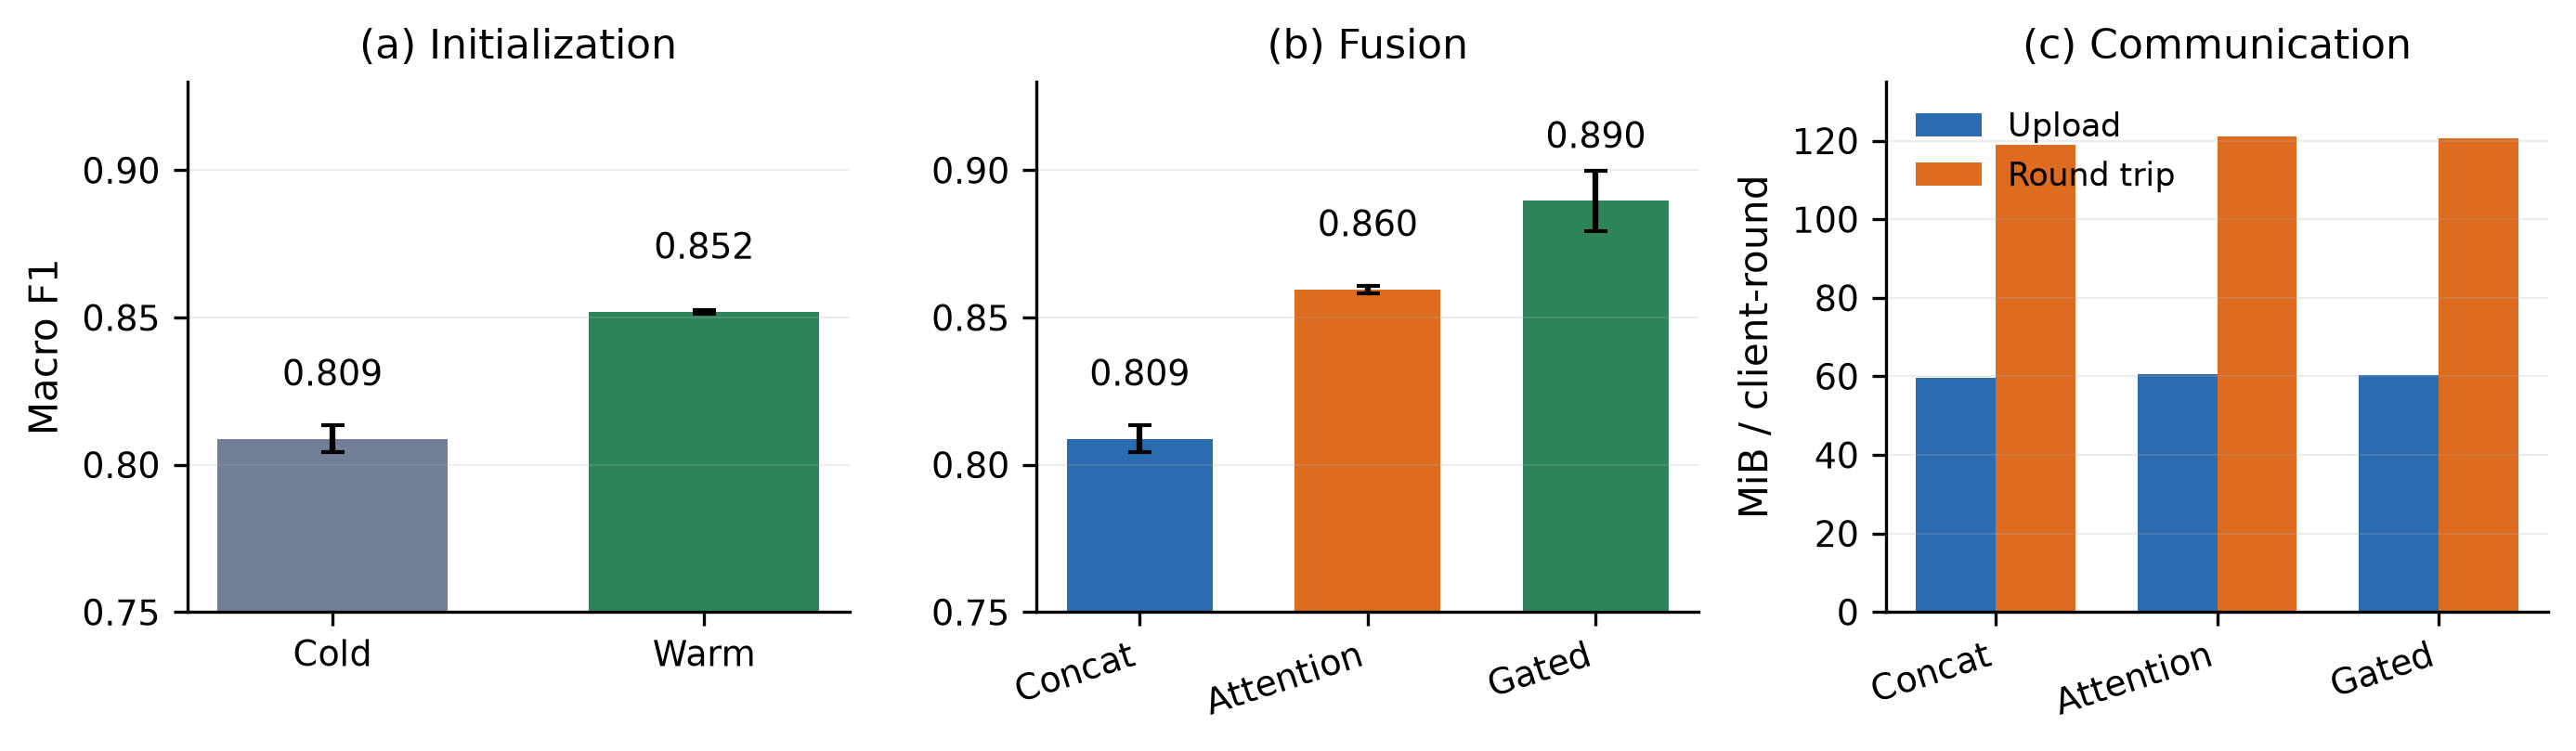
\includegraphics[width=0.6600\textwidth]{plots/plot82_remaining_ablations}
\caption{Remaining matched-setting ablations (two-seed means with standard
deviation bars): warm versus cold initialization, fusion strategy, and analytic
float32 communication per client-round.}
\label{fig:remaining_ablations}
\end{figure*}
\fi
%%TRIM-END%%


%%TRIM-BEGIN%% restore by deleting this line and the matching TRIM-END
\iffalse
\begin{figure*}[t]
\centering
%% The four panels are the quadrants of the rendered grid, laid out on one line.
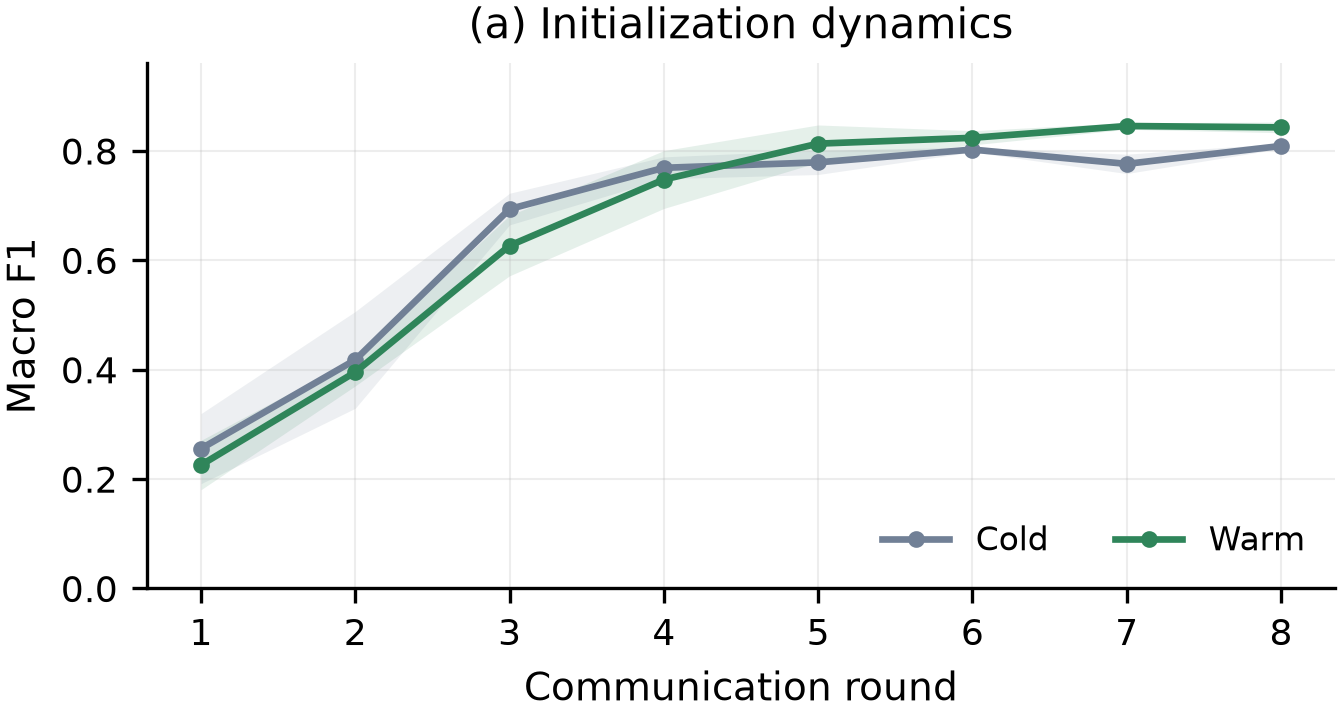
\includegraphics[width=0.2090\textwidth]{plots/plot83_a}\hfill
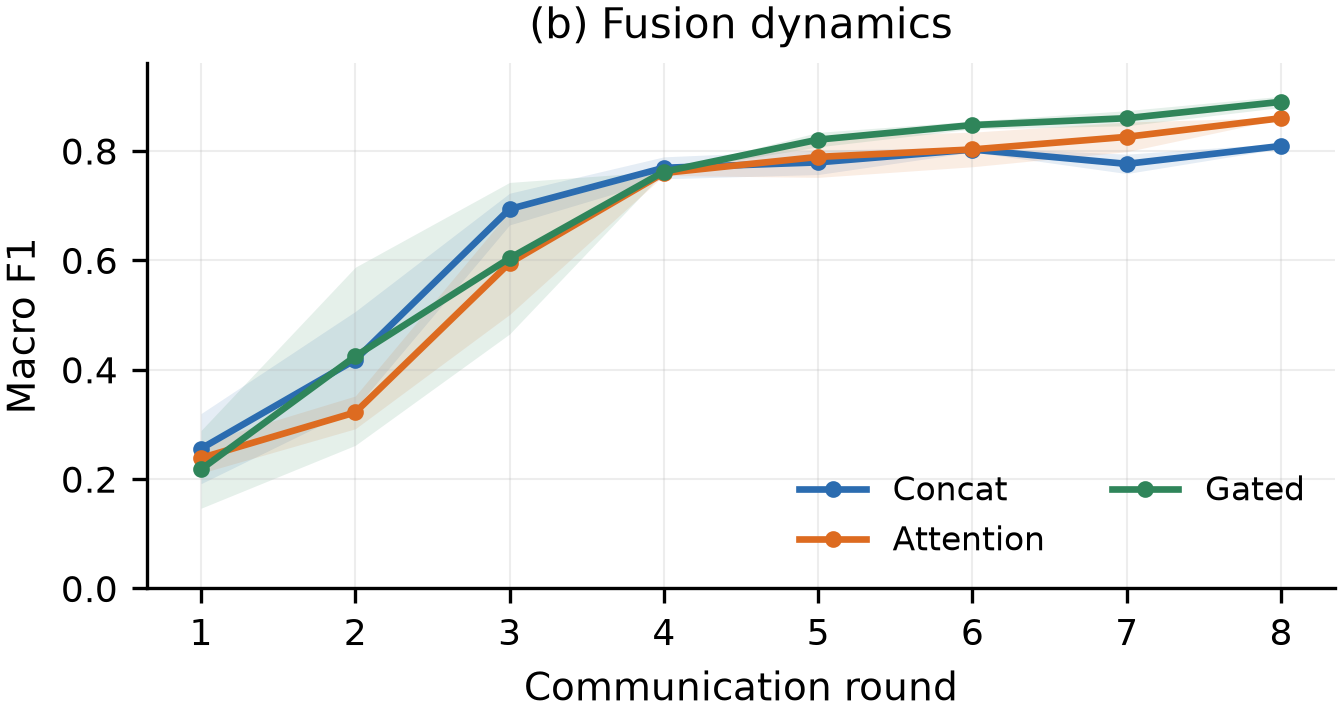
\includegraphics[width=0.2090\textwidth]{plots/plot83_b}\hfill
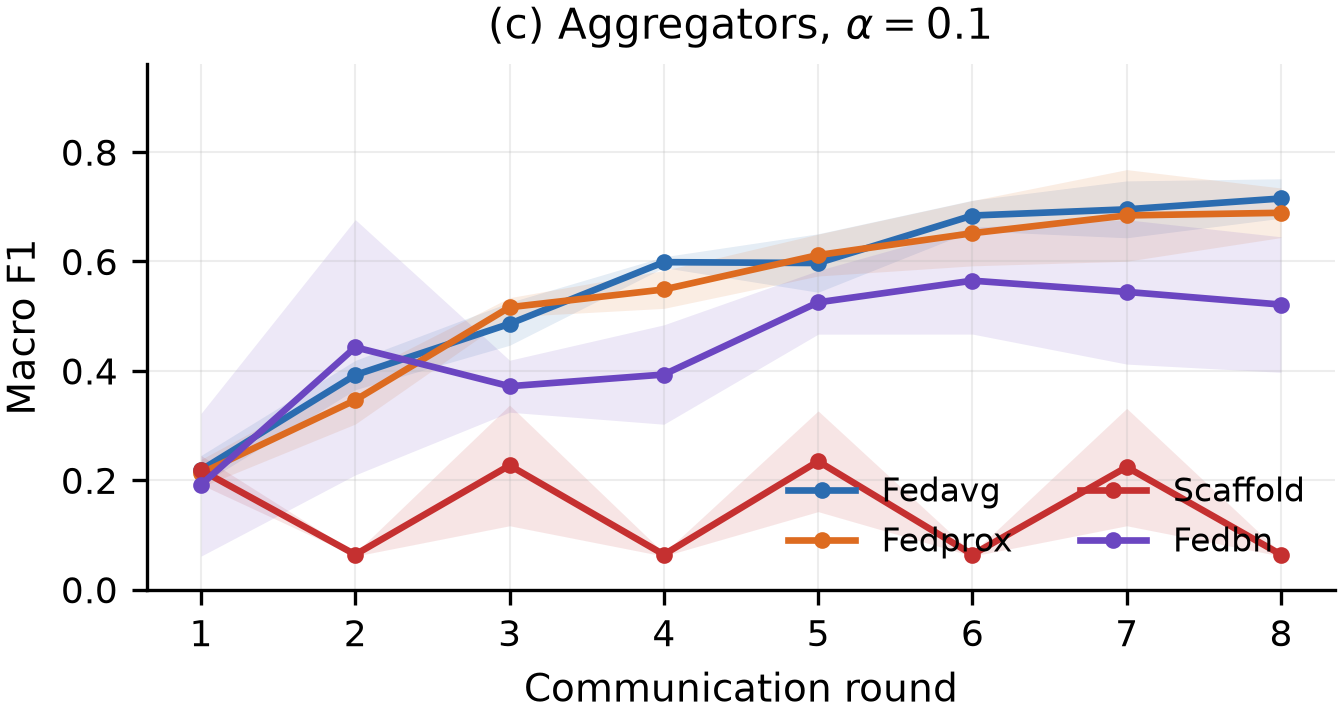
\includegraphics[width=0.2090\textwidth]{plots/plot83_c}\hfill
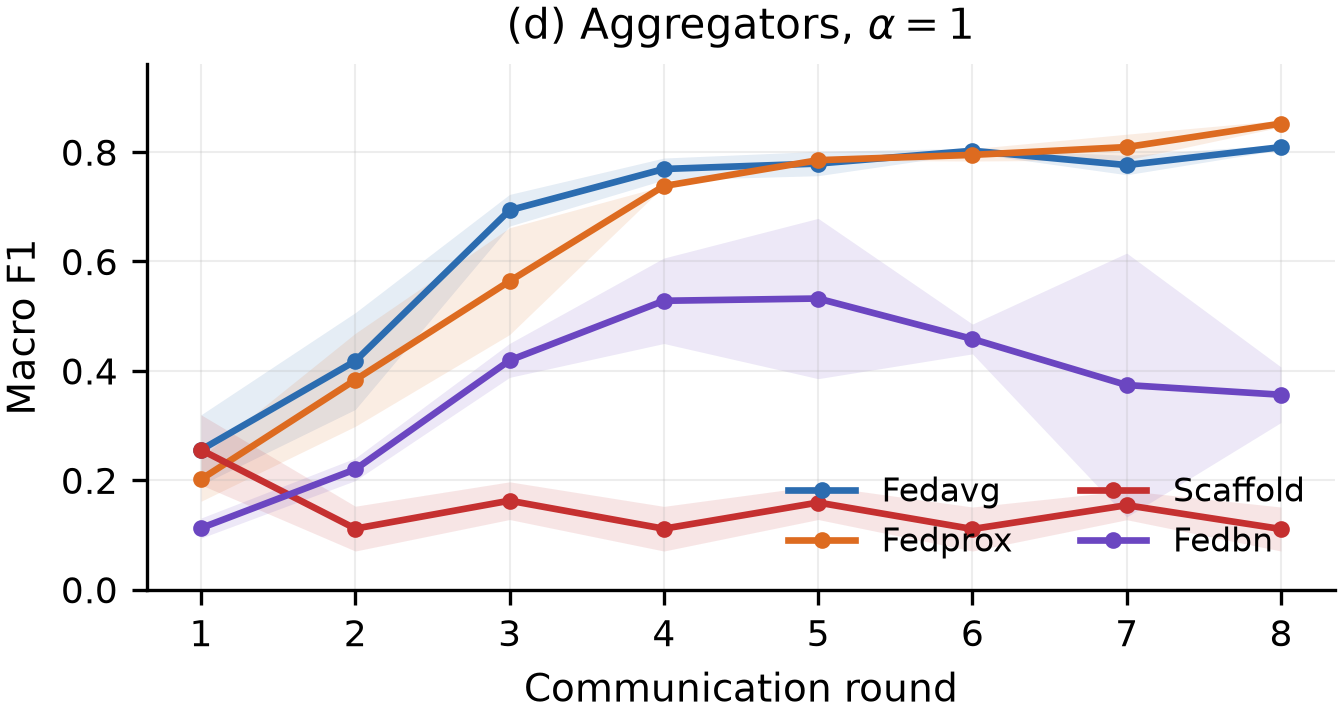
\includegraphics[width=0.2090\textwidth]{plots/plot83_d}
\caption{Round-wise matched-setting dynamics. Lines are two-seed means and
shading spans the observed seed range. Warm start separates late, gated fusion
finishes highest, FedAvg/FedProx converge under both skews, and SCAFFOLD remains
unstable on this support.}
\label{fig:training_dynamics}
\end{figure*}
\fi
%%TRIM-END%%


%%COMPACT-BEGIN%%
\begin{figure}[t]
\centering

\includegraphics[width=\figw]{plots/c16_cost_pareto}
\caption{Uplink cost against accuracy at $\alpha{=}0.1$; the line orders
architectures by uplink rather than interpolating. Cost spans $3.5\times$,
accuracy 0.073.}
\label{fig:c_cost}
\end{figure}
%%COMPACT-END%%

%%COMPACT-BEGIN%%
\begin{figure}[t]
\centering

\includegraphics[width=\figw]{plots/c24_anticollapse_arms}
\caption{Anti-collapse arms at both skews, from zero because the finding is
that none of them collapses. Values are printed: the arms span 0.044, all of it
the balanced sampler, and the diversity term does nothing.}
\label{fig:c_anticollapse}
\end{figure}
%%COMPACT-END%%

%%COMPACT-BEGIN%%
\begin{figure}[t]
\centering

\includegraphics[width=\figw]{plots/c25_seed_floor}
\caption{Every single-architecture matched-setting arm: bars are 3-seed means,
whiskers the observed seed range. The cold and concat arms are the same runs.
The ranges overlap, so no arm clears the spread.}
\label{fig:c_seed_floor}
\end{figure}
%%COMPACT-END%%


Table~\ref{tab:standard_suite} closes the remaining gaps without mixing
supports. The note correction rewrote text only, so the corrected splitter
still realizes label TV 0.451 against 0.265 at $\alpha=0.1$. Federation beats local-only training for all five architectures ($+$0.124 to
$+$0.229), and the ordering is architectural rather than the note-leakage
ceiling the previous corpus imposed. No aggregator dominates --- FedProx leads on
both fusion variants, FedAvg on image-only and cross-attention, FedBN on text
--- while SCAFFOLD is unstable everywhere (0.130--0.294). Communication
spans $3.5\times$, 18.9 to 67.2\,MiB per client-round, so image-only reaches
0.513 macro F1 at roughly a third the uplink of either fusion
(Fig.~\ref{fig:c_cost}).
Two arms report nothing, shown rather than asserted: the anti-collapse
components move the mean by at most 0.044 (Fig.~\ref{fig:c_anticollapse}), and
warm start leads on two of three seeds but loses the mean by 0.006, with the
fusion variants inside the same seed spread (Fig.~\ref{fig:c_seed_floor}).
Neither is claimed necessary.

%% generated by experiments/make_all_systems_table.py -- do not hand-edit

\begin{table}[t]
\caption{Frozen-encoder SGD heads on the shared source-grouped split. Each cell averages 18 runs (three seeds, six client counts; 50 rounds). Local denotes no communication; client partitions are matched within each cell.}
\label{tab:all_systems_fed}
\centering\footnotesize
\setlength\tabcolsep{4.0pt}
\begin{tabular}{lcccc}
\toprule
& \multicolumn{2}{c}{$\alpha=0.1$} & \multicolumn{2}{c}{$\alpha=1$}\\
\cmidrule(lr){2-3}\cmidrule(lr){4-5}
System & FedAvg & Local & FedAvg & Local\\
\midrule
Text (frozen DistilBERT) & 0.607 & 0.266 & 0.628 & 0.298\\
Image (frozen ViT-tiny) & 0.508 & 0.323 & 0.559 & 0.391\\
ViT$+$DistilBERT fusion & \textbf{0.723} & 0.317 & \textbf{0.775} & 0.364\\
\midrule
ResNet$+$compact (warm) & \multicolumn{4}{c}{0.892--0.910 over 2--8 clients}\\
\bottomrule
\end{tabular}
\end{table}

%%TRIM-BEGIN%% restore by deleting this line and the matching TRIM-END
\iffalse
\begin{figure}[t]
\centering
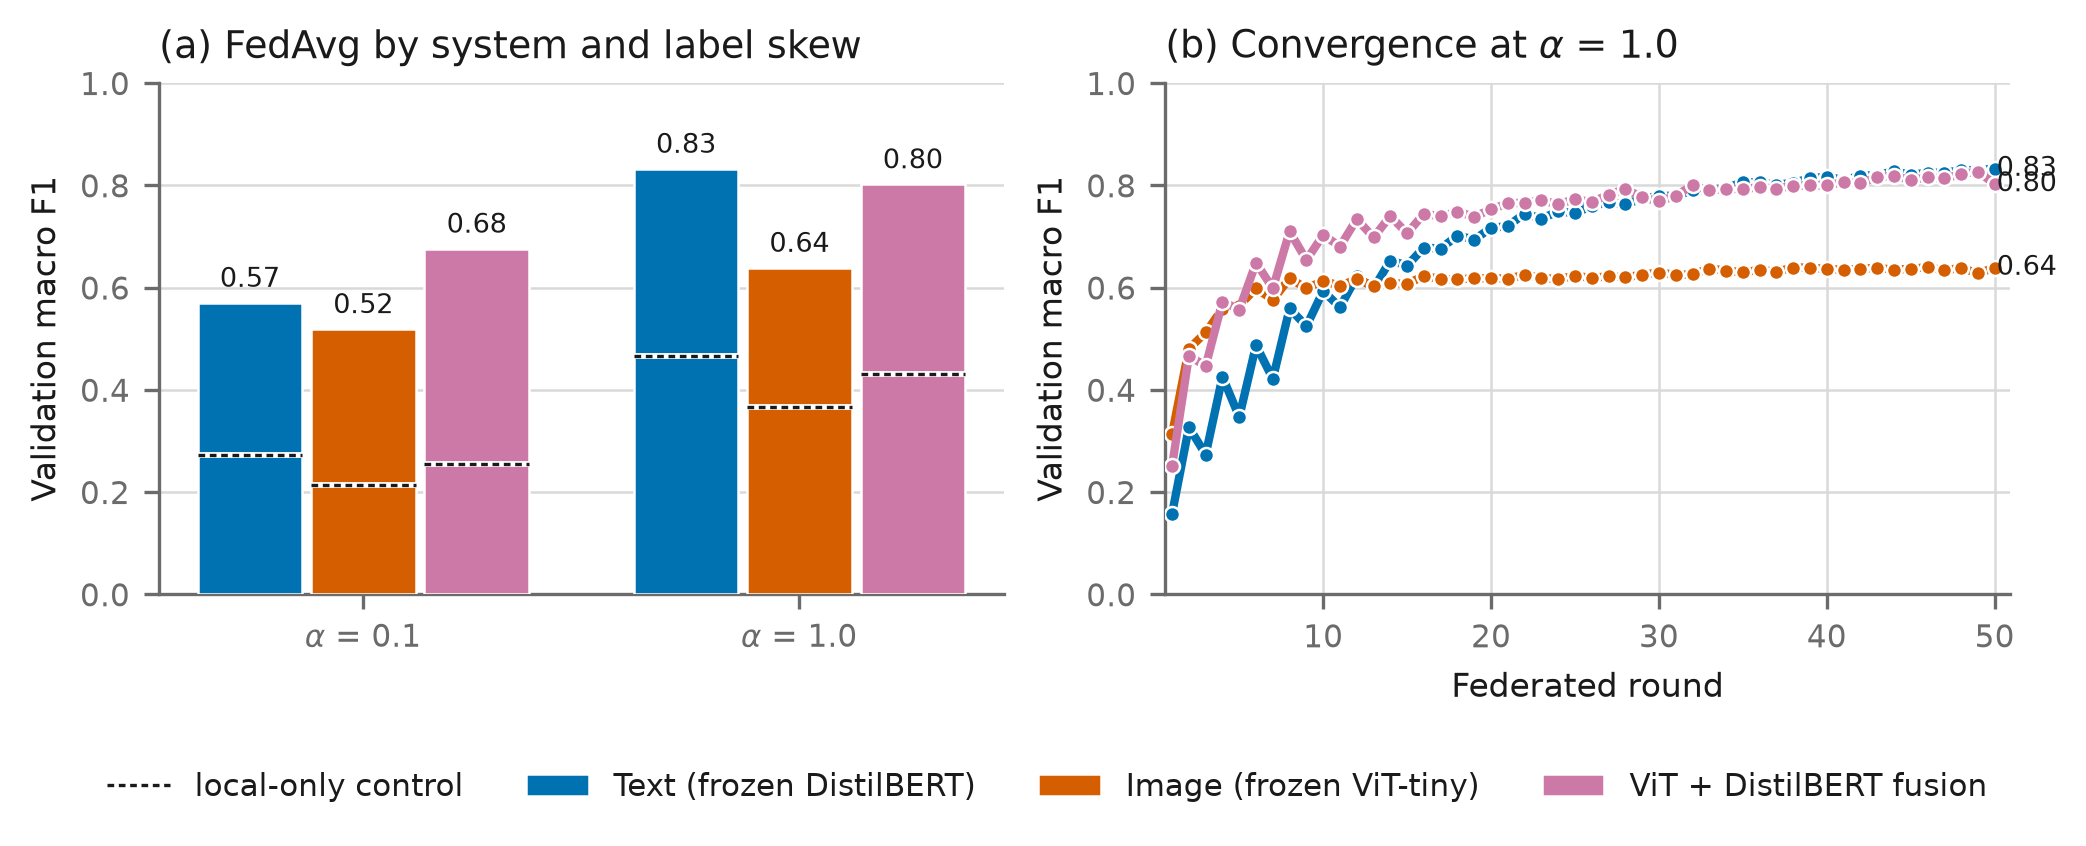
\includegraphics[width=\linewidth]{plots/plot80_federated_all_systems}
\caption{Per-system federated adaptation. (a) FedAvg macro F1 by system and
label skew; the dashed rule inside each bar is that system's local-only control,
so the bar above it is the federation gain. (b) Per-round convergence at
$\alpha=1$. Every system in a cell trains on the identical client partition.}
\label{fig:all_systems_fed}
\end{figure}
\fi
%%TRIM-END%%


%%COMPACT-BEGIN%%
\begin{figure}[t]
\centering

\includegraphics[width=\figw]{plots/c14_round_curves}
\caption{Rounds against performance for the frozen-encoder systems at
$\alpha{=}1$ (three seeds $\times$ six client counts). Fusion leads at every
round: 0.775 against 0.628 text and 0.559 image.}
\label{fig:c_round_curves}
\end{figure}
%%COMPACT-END%%

%%COMPACT-BEGIN%%
\begin{figure}[t]
\centering

\includegraphics[width=\figw]{plots/c15_client_scaling}
\caption{The same systems against client count. Fusion leads at every count,
0.734--0.799 against 0.587--0.689 for text.}
\label{fig:c_client_scaling}
\end{figure}
%%COMPACT-END%%



%% STALE -- DO NOT RESTORE AS-IS: predates the note-leakage
%% correction (caption asserts 1.0); regenerate the plot
%% from current data and rewrite the caption first.
%%TRIM-BEGIN%% restore by deleting this line and the matching TRIM-END
\iffalse
\begin{figure}[t]
\centering
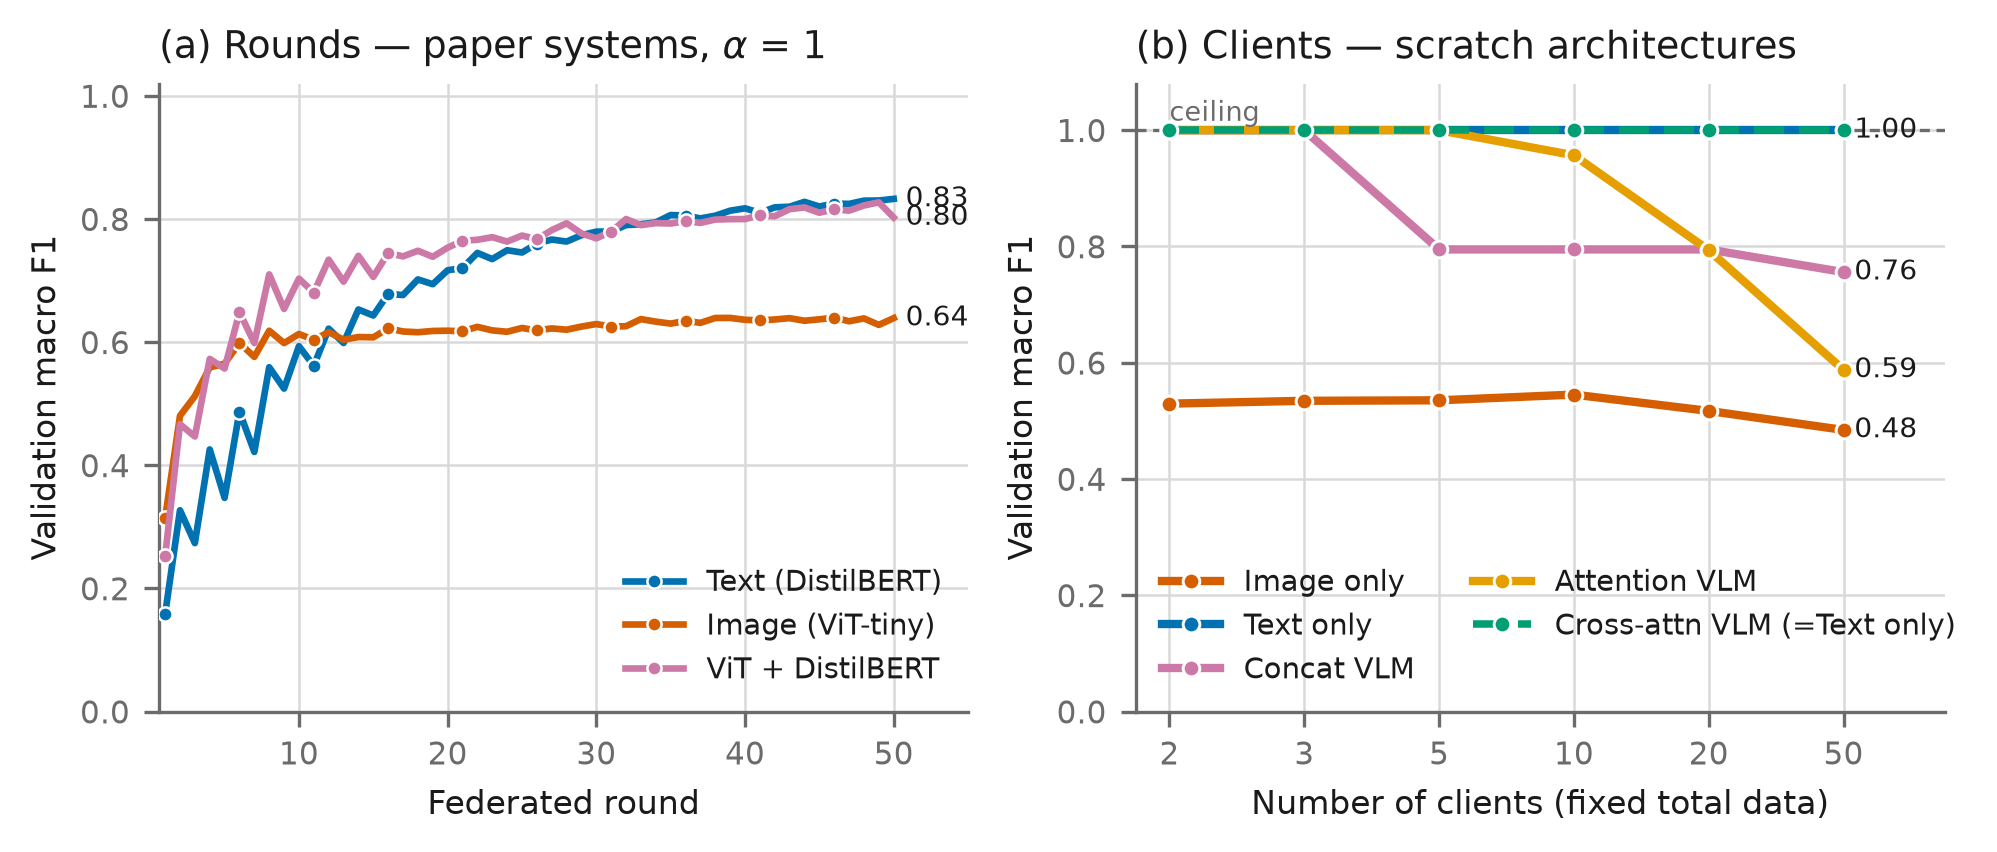
\includegraphics[width=\linewidth]{plots/plot81_federated_rounds_clients}
\caption{Federated rounds and client scaling. (a) Per-round convergence of the
paper's systems at $\alpha=1$; fusion overtakes both parents after round five.
(b) Macro F1 against the number of clients the same fixed training data is split
across, for the scratch architectures. Text-only and cross-attention coincide at
every client count, so the latter is drawn dashed; both sit at the 1.000 ceiling
until $K=10$, which is the saturation the text discusses rather than a scaling
result.}
\label{fig:fed_rounds_clients}
\end{figure}
\fi
%%TRIM-END%%


Table~\ref{tab:all_systems_fed} extends the federated evidence beyond one
architecture. A closed-form ridge head has no gradients for FedAvg to average,
so these systems are federated as linear probes --- frozen encoder, SGD head ---
which is not the centralized estimator. Within this protocol fusion leads at both skews (0.723 against 0.607 for
text and 0.508 for image at $\alpha=0.1$; 0.775, 0.628 and 0.559 at
$\alpha=1$) and takes the largest federation gain over local-only training in
both cells ($+0.406$ and $+0.411$), and it holds at every round
(Fig.~\ref{fig:c_round_curves}) and every client count: at $\alpha=1$ fusion
spans 0.734--0.799 from $K=2$ to 50, above text (0.587--0.689) throughout
(Fig.~\ref{fig:c_client_scaling}). Combining the
branches therefore helps most exactly where partitioning is most severe. Client partitions remain simulated.

%%TRIM-BEGIN%% restore by deleting this line and the matching TRIM-END
\iffalse
\begin{figure*}[t]
\centering
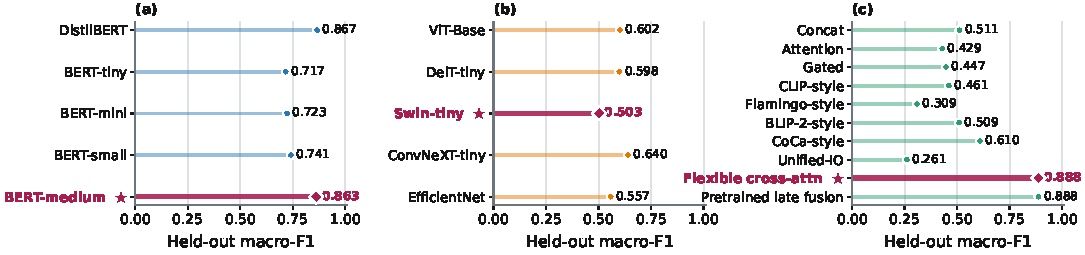
\includegraphics[width=0.7367\textwidth]{plots/plot75_within_family_models}\\[-1mm]
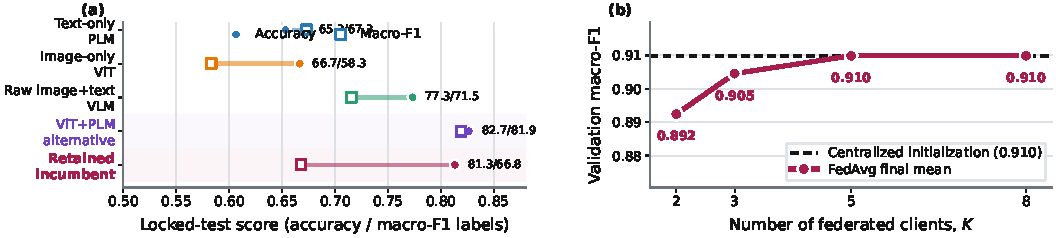
\includegraphics[width=0.7367\textwidth]{plots/plot76_current_intermodel_and_central_fed}
\caption{Model comparisons retained as visual evidence. Top: within-family
screens on their own supports (cross-panel scores are not comparable). Bottom:
common 75-crop support for selected PLM, ViT, raw VLM, candidate VLM, and retained
system (left), plus three-seed warm-start FedAvg scaling (right).}
\label{fig:model_comparisons}
\end{figure*}
\fi
%%TRIM-END%%


\subsection{Same-Checkpoint Ablation and Image-Only Gains}

%%TRIM-BEGIN%% restore by deleting this line and the matching TRIM-END
\iffalse
\begin{table}[t]
\centering
\caption{Same-checkpoint ablation and configuration guidance. One core, one
75-crop support, two note conditions. Bold marks the configuration to use for
the evidence each block assumes; the reversal between blocks is the result.}
\label{tab:standard_ablation}
\scriptsize
\setlength{\tabcolsep}{3.2pt}
\begin{tabular}{lrrrr}
\toprule
Condition & Accuracy & Correct & Macro F1 & ECE \\
\midrule
\multicolumn{5}{l}{\emph{Complete notes --- use text alone}}\\
Core image path (ResNet) & 0.6133 & 46/75 & 0.5431 & 0.1135 \\
Core text path (compact Tr.) & \textbf{0.9600} & 72/75 & \textbf{0.9049} & 0.1463 \\
Base paired VLM   & 0.9200 & 69/75 & 0.8753 & 0.2648 \\
Mismatched-pair VLM & 0.3333 & 25/75 & 0.2804 & 0.2193 \\
\midrule
\multicolumn{5}{l}{\emph{Half-masked notes --- use the router}}\\
Text alone      & 0.6400 & 48/75 & 0.5798 & --\\
Visual gate     & 0.7200 & 54/75 & 0.6759 & --\\
Plain fusion    & 0.7867 & 59/75 & 0.6472 & --\\
Routed fusion   & \textbf{0.8133} & 61/75 & 0.6679 & --\\
\bottomrule
\end{tabular}
\end{table}
\fi
%%TRIM-END%%


Both branches carry evidence and neither dominates: unimodally the image leads
this test 0.6400 against 0.2400, and Section~\ref{sec:modality_inertness}
quantifies both ablations. Notes are templated, so every note-side number is an
upper bound, and the routing family was refined on this partition. A validation-selected test-time-augmentation search over 25 view/scale
candidates reaches 74.32\% validation accuracy (macro F1 0.6854) with the
base, tight-crop and context-crop views, and 64.00\% on the locked test (macro F1 0.5532).
This is an inference-time ensemble over one backbone, not a stronger encoder;
rare-class behaviour remains unstable.

%% STALE -- DO NOT RESTORE AS-IS: predates the note-leakage
%% correction (caption asserts curves coinciding at 1.000); regenerate the plot
%% from current data and rewrite the caption first.
%%TRIM-BEGIN%% restore by deleting this line and the matching TRIM-END
\iffalse
\begin{figure}[t]
\centering

\includegraphics[width=\linewidth]{plots/plot82_clubbed_modality}
\caption{Clubbed modality comparison on the common 75-crop support. (a) The classical feature baseline beside the best pretrained system per modality at 50\% note deletion: pretraining is decisive on images (0.440 to 0.733) and is not on text, where TF-IDF leads every transformer encoder. (b) Test accuracy as field notes are removed, colour by modality and line style by deployment. The text and fusion curves coincide exactly at 1.000 with complete notes, so one marker hides the other there; they separate as notes are deleted, while the image branch is flat by construction.}
\label{fig:clubbed_modality}
\end{figure}
\fi
%%TRIM-END%%


\begin{table*}[t]
\caption{Unimodal systems on the same 222/74/75 split, crop-linked notes, and train-fitted mask. Test metrics use validation-selected configurations. FedAvg uses five Dirichlet($\alpha=1$) clients, 50 rounds, and three seeds. Centralized heads are closed-form; federated heads use SGD. Image rows are invariant to note deletion. Bold: best per block/column.}
\label{tab:unimodal_cent_fed}
\centering\footnotesize
\setlength\tabcolsep{4pt}
\begin{tabular}{lrcccccccccccc}
\toprule
 &  & \multicolumn{4}{c}{Complete notes} & \multicolumn{4}{c}{50\% of notes deleted} & \multicolumn{4}{c}{75\% of notes deleted}\\
\cmidrule(lr){3-6}\cmidrule(lr){7-10}\cmidrule(lr){11-14}
 &  & \multicolumn{2}{c}{Centralized} & \multicolumn{2}{c}{Federated} & \multicolumn{2}{c}{Centralized} & \multicolumn{2}{c}{Federated} & \multicolumn{2}{c}{Centralized} & \multicolumn{2}{c}{Federated}\\
\cmidrule(lr){3-4}\cmidrule(lr){5-6}\cmidrule(lr){7-8}\cmidrule(lr){9-10}\cmidrule(lr){11-12}\cmidrule(lr){13-14}
System & Dim. & Acc. & F1 & Acc. & F1 & Acc. & F1 & Acc. & F1 & Acc. & F1 & Acc. & F1\\
\midrule
\multicolumn{14}{l}{\emph{Text only}}\\
TF-IDF $+$ linear SVM & 864 & \textbf{0.640} & 0.503 & \textbf{0.582} & \textbf{0.469} & \textbf{0.493} & \textbf{0.390} & \textbf{0.476} & \textbf{0.375} & \textbf{0.373} & \textbf{0.298} & \textbf{0.360} & \textbf{0.293}\\
BERT-tiny & 128 & 0.613 & 0.508 & 0.440 & 0.332 & 0.400 & 0.316 & 0.324 & 0.251 & 0.320 & 0.204 & 0.276 & 0.196\\
BERT-mini & 256 & 0.613 & 0.496 & 0.427 & 0.331 & 0.427 & 0.318 & 0.440 & 0.332 & 0.280 & 0.186 & 0.276 & 0.190\\
BERT-small & 512 & \textbf{0.640} & \textbf{0.512} & 0.564 & 0.467 & 0.427 & 0.306 & 0.431 & 0.331 & \textbf{0.373} & 0.291 & 0.253 & 0.197\\
BERT-medium & 512 & 0.600 & 0.493 & 0.529 & 0.426 & 0.333 & 0.254 & 0.400 & 0.309 & 0.253 & 0.158 & 0.213 & 0.185\\
DistilBERT & 768 & 0.613 & 0.485 & 0.529 & 0.422 & 0.427 & 0.328 & 0.431 & 0.332 & 0.360 & 0.286 & 0.249 & 0.194\\
\midrule
\multicolumn{14}{l}{\emph{Image only}}\\
Colour$+$HOG SVM & 630 & 0.440 & 0.346 & 0.471 & 0.392 & 0.440 & 0.346 & 0.471 & 0.392 & 0.440 & 0.346 & 0.471 & 0.392\\
Swin-tiny & 768 & 0.600 & 0.507 & 0.569 & 0.463 & 0.600 & 0.507 & 0.569 & 0.463 & 0.600 & 0.507 & 0.569 & 0.463\\
ConvNeXT-tiny & 768 & 0.560 & 0.493 & 0.560 & 0.470 & 0.560 & 0.493 & 0.560 & 0.470 & 0.560 & 0.493 & 0.560 & 0.470\\
EfficientNet-B0 & 1280 & 0.680 & 0.561 & \textbf{0.680} & 0.573 & 0.680 & 0.561 & \textbf{0.680} & 0.573 & 0.680 & 0.561 & \textbf{0.680} & 0.573\\
DeiT-tiny & 192 & 0.693 & 0.545 & 0.636 & 0.520 & 0.693 & 0.545 & 0.636 & 0.520 & 0.693 & 0.545 & 0.636 & 0.520\\
ViT-Base/16 & 768 & \textbf{0.733} & \textbf{0.615} & 0.667 & \textbf{0.577} & \textbf{0.733} & \textbf{0.615} & 0.667 & \textbf{0.577} & \textbf{0.733} & \textbf{0.615} & 0.667 & \textbf{0.577}\\
\bottomrule
\end{tabular}
\end{table*}

\begin{table*}[t]
\caption{Multimodal systems under the protocol of Table~\ref{tab:unimodal_cent_fed}. Best unimodal references appear below. Complete-note fusion reaches 0.800 versus 0.733 image-only and 0.640 text-only. Bold: best per column.}
\label{tab:multimodal_cent_fed}
\centering\footnotesize
\setlength\tabcolsep{4pt}
\begin{tabular}{lrcccccccccccc}
\toprule
 &  & \multicolumn{4}{c}{Complete notes} & \multicolumn{4}{c}{50\% of notes deleted} & \multicolumn{4}{c}{75\% of notes deleted}\\
\cmidrule(lr){3-6}\cmidrule(lr){7-10}\cmidrule(lr){11-14}
 &  & \multicolumn{2}{c}{Centralized} & \multicolumn{2}{c}{Federated} & \multicolumn{2}{c}{Centralized} & \multicolumn{2}{c}{Federated} & \multicolumn{2}{c}{Centralized} & \multicolumn{2}{c}{Federated}\\
\cmidrule(lr){3-4}\cmidrule(lr){5-6}\cmidrule(lr){7-8}\cmidrule(lr){9-10}\cmidrule(lr){11-12}\cmidrule(lr){13-14}
System & Dim. & Acc. & F1 & Acc. & F1 & Acc. & F1 & Acc. & F1 & Acc. & F1 & Acc. & F1\\
\midrule
\multicolumn{14}{l}{\emph{Multimodal (image $+$ text)}}\\
TF-IDF $+$ Colour/HOG SVM & 1494 & 0.667 & 0.537 & 0.631 & 0.526 & 0.587 & 0.480 & 0.547 & 0.451 & 0.547 & 0.451 & 0.449 & 0.381\\
ViT-Base $+$ BERT-tiny & 896 & 0.747 & 0.625 & \textbf{0.693} & 0.597 & \textbf{0.733} & \textbf{0.614} & \textbf{0.684} & \textbf{0.645} & 0.600 & 0.513 & 0.698 & 0.610\\
ViT-Base $+$ BERT-mini & 1024 & 0.773 & 0.643 & 0.676 & 0.585 & 0.667 & 0.574 & \textbf{0.684} & 0.619 & \textbf{0.787} & \textbf{0.655} & \textbf{0.716} & \textbf{0.614}\\
ViT-Base $+$ BERT-small & 1280 & \textbf{0.800} & \textbf{0.664} & 0.667 & \textbf{0.600} & 0.627 & 0.543 & 0.631 & 0.545 & 0.613 & 0.528 & 0.676 & 0.572\\
ViT-Base $+$ BERT-medium & 1280 & 0.773 & 0.642 & 0.676 & 0.566 & 0.720 & 0.593 & 0.653 & 0.561 & 0.680 & 0.571 & 0.622 & 0.515\\
ViT-Base $+$ DistilBERT & 1536 & 0.773 & 0.645 & 0.653 & 0.553 & 0.693 & 0.579 & 0.636 & 0.554 & 0.693 & 0.581 & 0.640 & 0.531\\
\midrule
\multicolumn{14}{l}{\emph{Best unimodal system, repeated for reference}}\\
Text only: TF-IDF $+$ linear SVM & 864 & 0.640 & 0.503 & 0.582 & 0.469 & 0.493 & 0.390 & 0.476 & 0.375 & 0.373 & 0.298 & 0.360 & 0.293\\
Image only: ViT-Base/16 & 768 & 0.733 & 0.615 & 0.667 & 0.577 & 0.733 & 0.615 & 0.667 & 0.577 & 0.733 & 0.615 & 0.667 & 0.577\\
\bottomrule
\end{tabular}
\end{table*}

\subsection{Unimodal and Multimodal Systems, Centralized and Federated}




Tables~\ref{tab:unimodal_cent_fed} and~\ref{tab:multimodal_cent_fed} place a
classical feature baseline, five frozen text encoders, five frozen vision
encoders and their fusions on the same 222/74/75 support, scored centrally and
again under FedAvg.

\textbf{Unimodal.} With complete notes the image branch leads the text branch: ViT-Base reaches
0.733 against 0.640 for the best text encoder, BERT-small. Federating costs
little on either side (0.733 to 0.667; 0.640 to 0.582), so the modality
separates these systems, not the deployment mode. The classical rows locate
where pretraining earns its place: decisive on images (0.440 against 0.733) and
absent on text, where TF-IDF with a linear SVM ties the best transformer at
0.640. Neither branch is near the
ceiling, so the comparison is informative rather than saturated.

\textbf{Multimodal.} Fusion beats both parents outright, and does so at complete notes:
ViT-Base with BERT-small reaches 0.800 against 0.733 for the best image-only
encoder and 0.640 for the best text-only encoder. All five ViT-Base$+$BERT rows clear the best
unimodal system (lowest 0.747 against 0.733), so the gain is not one lucky
pairing; the classical TF-IDF with colour/HOG fusion does not,
placing the gain in the pretrained encoders rather than in concatenation. The
advantage widens as notes degrade: at 75\% deletion text falls to 0.373 while
fusion holds 0.787 and the image branch is unmoved by construction. Federation preserves
the ordering rather than creating it, and its cost falls as the note thins ---
0.800 to 0.667 at complete notes, 0.787 to 0.716 at 75\% deletion.

Every ViT-Base pairing outperforms the best text-only system at every sparsity level,
but the best text partner changes: BERT-small leads with complete notes,
while BERT-mini leads at 75\% sparsity. The performance spread across the five
pairings widens from 0.053 to 0.187. These results support fusion over its
unimodal parents, but do not identify a consistently best text encoder.

\subsection{Robustness: Skew, Dropout, Stragglers and Poisoning}
\label{sec:robustness}

\begin{figure*}[t]
\centering

\includegraphics[width=0.80\textwidth]{plots/plot91_robustness_stragglers_poison}
\caption{Federated failure modes on the audited split. (a) Label skew from
$\alpha{=}10$ to one class per client. (b) Clients reporting an update computed from
an earlier global model. (c) Malicious clients under mean against
coordinate-wise-median aggregation. Bands are $\pm$1 SD over 3 seeds. Client
dropout is omitted because it is flat to 70\%; the released figure set carries it.}
\label{fig:robustness}
\end{figure*}



\textbf{Skew and dropout break nothing} (Fig.~\ref{fig:robustness}a)\textbf{.} From $\alpha{=}10$ down to
$\alpha{=}0.01$, and under a pathological partition giving each client a
single class, fused macro-F1 stays in 0.741--0.776 --- its worst setting above
the best setting of either parent (0.617 text, 0.660 image). Dropout is
flatter still: 70\% of clients failing to report each round leaves the fused
system at 0.773 against 0.772 with none. The image branch is the limiting case: a convex
probe returns per-seed-identical scores across $\alpha{=}0.5$, 1 and 10 and again
across $\alpha{=}0.05$, 0.01 and the pathological split, so skew changes the path
and not the destination.

\textbf{Stragglers cost what dropout does not} (Fig.~\ref{fig:robustness}b). A
stale update arrives and is averaged in, pulling the model toward an older
global state rather than merely shrinking the cohort. At 75\% stale updates per
round the fused system loses 0.115 (0.772 to 0.657) and the image branch 0.123
(0.660 to 0.537), where the same fraction of \emph{dropped} clients costs
nothing. Discarding a late update beats waiting for it.

\textbf{Poisoning is where plain FedAvg has no defence} (Fig.~\ref{fig:robustness}c). Sign-flipped updates are
catastrophic at every fraction: 10\% malicious clients take the fused system
from 0.772 to 0.298 and 30\% to 0.123, with text (0.136) and image (0.104)
equally destroyed --- the one condition in which fusion is not best, because all
three are broken. Label
flip degrades gradually instead (0.658, 0.611, 0.539 at 10/20/30\%) and
Gaussian noise sits between them. Coordinate-wise median recovers the outlier
attacks (sign flip to 0.613, 0.543, 0.420) but not label flip, which is worse at
30\% (0.510 against 0.539): a label-flipped update is a well-formed gradient step
toward the wrong target, not an outlier in parameter space. The median also costs
0.057 with nobody attacking, so it is a trade, not a free defence. Nothing here
is Byzantine-tolerant.



\subsection{Actual Model-Family and Inter-Model Comparison}




%% generated by experiments/make_encoder_selection_table.py -- do not hand-edit

%% generated by experiments/make_encoder_selection_table.py -- do not hand-edit

%% generated by experiments/make_encoder_selection_table.py -- do not hand-edit

\begin{table}[t]
\caption{Validation-only family selection; test follows selection. Sparse-note retention is 15\%. The image baseline is ViT-tiny, unlike ViT-Base in Table~\ref{tab:unimodal_cent_fed}.}
\label{tab:family_comparison}
\centering\footnotesize
\setlength\tabcolsep{3.8pt}
\begin{tabular}{lccc}
\toprule
\textbf{Actual system} & \textbf{Val. acc.} & \textbf{Test acc.} & \textbf{Test F1}\\
\midrule
Text PLM (DistilBERT) & 0.2297 & 0.2400 & 0.2167\\
Image ViT (ViT-tiny) & 0.7432 & \textbf{0.6400} & \textbf{0.5532}\\
Raw ResNet$+$compact VLM & 0.7568 & 0.5867 & 0.5076\\
ViT$+$DistilBERT VLM & 0.7297 & \textbf{0.6400} & 0.5334\\
Routed ResNet$+$compact (LEAF) & \textbf{0.7703} & 0.6133 & 0.5319\\
\bottomrule
\end{tabular}
\end{table}



In Table~\ref{tab:family_comparison} the routed ResNet--compact model, LEAF, is the
\emph{incumbent} --- the core already carried into the routing and federated
experiments --- and the pooled ViT--DistilBERT model is the \emph{candidate},
adopted only if it beats the incumbent on validation. Validation selects the
incumbent before test extraction: 77.03\% accuracy and 0.7169 F1
against 72.97\% and 0.5980 for the candidate. On test the candidate
predicts 2 more crops, but the 11-versus-9 discordance is not
significant (McNemar $p=0.82$) and the two macro-F1 values differ by
0.0014. On 75 crops the support does not separate them, so the
selection rule decides and the test column is reported rather than ranked. The
enhanced gate gains eight correct crops over the direct image path and the
router 15, mainly in blight and looper; two leaf-hopper crops are too few to
carry a claim.

\subsection{Missing-Modality and Corruption Probes}
\label{sec:modality_inertness}

Mismatching the note costs only 2.67 accuracy points and 0.0187 F1, and exact
cross-modal recall@1 is 1.33\% against class-level 0.600/0.613: the embedding is
organized by class, not by crop identity.




The mismatch result shows dependence on the note, not whether the image is used
at all. We evaluate the retained checkpoint on the locked 75-crop test under
graded corruption of each modality and two full image ablations, comparing
predictions crop-by-crop against the clean run.

\textbf{Both branches are load-bearing.} Table~\ref{tab:corruption} reports the
sweep. Deleting every attended text token costs 0.226 macro F1 and moves
41 of 75 predictions; replacing the image with uniform noise costs 0.429
and moves 61. The image now carries more of the decision than the note,
reversing the previous corpus, but neither branch is inert. The reliability gate
does not track this: mean $w_t$ is 0.263 on clean input and rises to 0.361
under complete text deletion and 0.380 under complete image noise, so it
weights a destroyed modality more rather than less.

\textbf{Ablation strength determines the verdict.} Additive Gaussian noise at
$\sigma{=}0.35$ leaves leaf and lesion plainly visible and moves 25 of 75
predictions, whereas zeroing the image moves 49 and replacing it with uniform
noise moves 61. An earlier 30-pair proxy screen used the Gaussian setting alone
and read the visual branch as inert; that reading does not survive genuine
removal. Evidence that a branch is unused requires an ablation that removes it,
not one that degrades it.

%% generated by experiments/make_corruption_table.py -- do not hand-edit

%% generated by experiments/make_corruption_table.py -- do not hand-edit

%% generated by experiments/make_corruption_table.py -- do not hand-edit

\begin{table}[t]
\caption{Retained-checkpoint corruption on 75 locked test crops. Flips count changes from clean predictions. Full removal affects both modalities more strongly than partial corruption.}
\label{tab:corruption}
\centering\footnotesize
\setlength\tabcolsep{4pt}
\begin{tabular}{lccc}
\toprule
\textbf{Condition} & \textbf{Acc.} & \textbf{Macro F1} & \textbf{Flips}\\
\midrule
Clean & 0.6267 & 0.5163 & ---\\
\midrule
Text deletion 25\% & 0.6133 & 0.5060 & 4/75\\
Text deletion 50\% & 0.6267 & 0.5244 & 7/75\\
Text deletion 75\% & 0.6000 & 0.5068 & 11/75\\
Text deletion 100\% & 0.3600 & 0.2903 & 41/75\\
\midrule
Image Gaussian $\sigma{=}0.09$ & 0.6400 & 0.5234 & 13/75\\
Image Gaussian $\sigma{=}0.18$ & 0.6400 & 0.5308 & 16/75\\
Image Gaussian $\sigma{=}0.26$ & 0.6267 & 0.5247 & 17/75\\
Image Gaussian $\sigma{=}0.35$ & 0.5867 & 0.4906 & 25/75\\
\midrule
Image zeroed & 0.3733 & 0.1603 & 49/75\\
Image uniform noise & \textbf{0.2800} & 0.0875 & \textbf{61/75}\\
\bottomrule
\end{tabular}
\end{table}

\subsection{Fusing Text, Image and Weather}
\label{sec:weather_probe}

Field diagnosis is rarely made from a leaf alone: a scout reads the canopy
against the weather that produced it. We therefore extend the fusion to three
modalities, adding daily observations from the AMFU Kharagpur station
(IMD 42893) beside the note and the photograph. A small multilayer perceptron
embeds a $19$-dimensional standardized vector of temperature, humidity, rainfall
and its accumulations, rainless-spell length, vapour pressure deficit,
evaporation, soil temperature and sunshine; the router widens to
$r_t+r_v+r_w=1$ and the head gains one block.

The corpus records no capture date (Section~\ref{sec:dataset}), so each crop is
assigned a station day by hashing its (photograph, box index) pair
\emph{independently of its label}. We verify that independence: per-class mean
weather agrees to within $0.28\,^{\circ}$C and $0.43$\,h of sunshine, and the
share of crops whose assigned day is high-risk for their own class is $12.1\%$
against a $12.0\%$ base rate. The third modality is uninformative by
construction, which turns this into a test of the router with a known answer.

Figure~\ref{fig:weather_ablation} reports five seeds per arm. Accuracy is
unchanged, as it should be, and the spread across seeds is an order of magnitude
larger than any gap between the arms --- a single-seed comparison on $371$ crops
can move several points from noise alone. The informative result is that the
gate still assigns $0.16\pm0.03$ of its mass to the useless input rather than
the zero an ideal reliability estimate would give: nothing in the classification
objective drives such a weight to zero while the fusion head can compensate, so
the learned weights are diagnostics to inspect, not calibrated evidence.

\begin{figure}[t]
\centering
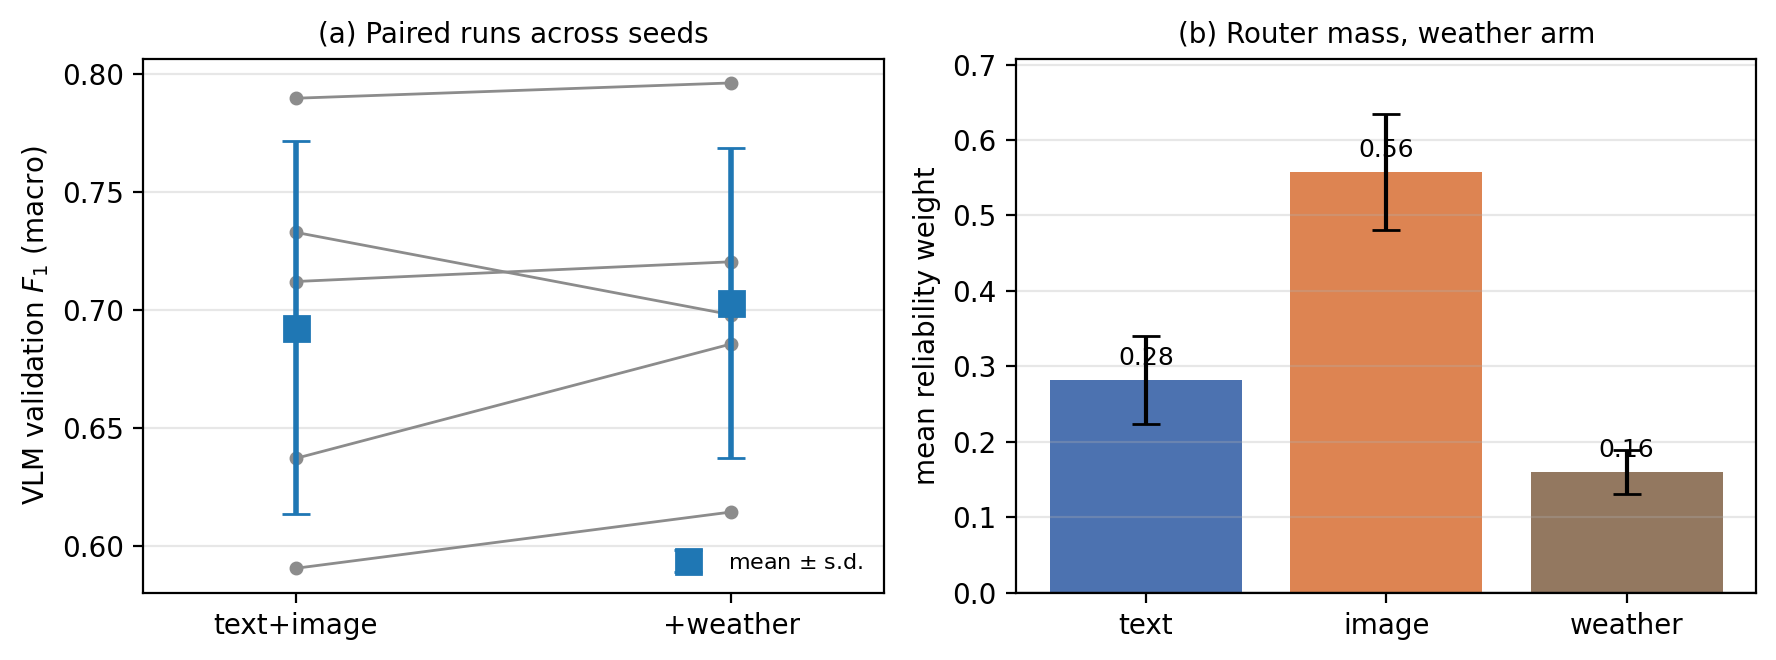
\includegraphics[width=0.99\linewidth]{plots/weather_ablation.png}
\footnotesize
\setlength\tabcolsep{3.5pt}
\begin{tabular}{lcc}
\toprule
Macro $F_1$ & Text$+$image & $+$weather\\
\midrule
Validation & $0.693 \pm 0.079$ & $0.703 \pm 0.066$\\
Federated  & $0.573 \pm 0.070$ & $0.576 \pm 0.097$\\
Test       & $0.570 \pm 0.080$ & $0.575 \pm 0.034$\\
\bottomrule
\end{tabular}
\caption{Adding weather as a third modality, five seeds per arm. (a) Paired
runs; grey lines join the arms for one seed, squares mark mean $\pm$ one
standard deviation. (b) Mean reliability mass per modality. Table: mean $\pm$
s.d.; every difference is at most a tenth of the pooled standard deviation while
the seed spread is $0.07$--$0.08$, so the arms are indistinguishable --- as they
must be, the assignment being label-independent. The router nonetheless gives
$0.16$ of its mass to the uninformative input.}
\label{fig:weather_ablation}
\end{figure}

\subsection{Architecture Component Ablation}
\label{sec:architecture_ablation}

Eleven variants $\times$ 3 seeds on one device (33 runs) separate component
effects from seed noise, which the earlier CPU-versus-H100 comparison
confounded. The floor is high: pooled within-variant SD is 0.032 accuracy and
the full model alone spans 0.053 across seeds (0.649 mean). One effect clears
it --- a lightweight vision encoder costs 0.227 --- and no other ablation moves
the mean by more than 0.071. The expert-residual weight is unsupported:
$\lambda{=}0$ ($-0.013$) beats $\lambda{=}1$ ($-0.044$) and $\lambda{=}4$ ($-0.040$)
against the $\lambda{=}2$ default, so the ordering is non-monotone. With a
frozen-encoder concatenation reaching 0.800 on the same support
(Table~\ref{tab:multimodal_cent_fed}), the trained architecture is not what
produces the multimodal result and is not claimed to be.

%%TRIM-BEGIN%% restore by deleting this line and the matching TRIM-END
\iffalse
\begin{figure*}[t]
\centering
\begin{subfigure}[b]{0.3434\textwidth}
  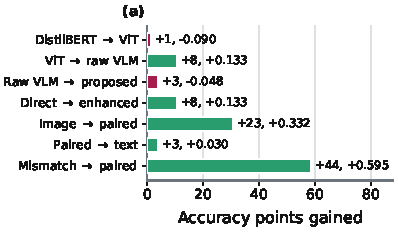
\includegraphics[width=\linewidth]{plots/plot78a_score_gains}
\end{subfigure}\hfill
\begin{subfigure}[b]{0.2207\textwidth}
  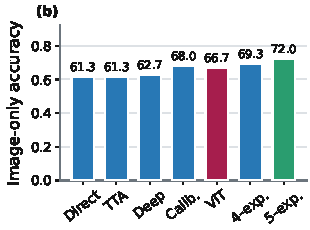
\includegraphics[width=\linewidth]{plots/plot78b_image_ladder}
\end{subfigure}\hfill
\begin{subfigure}[b]{0.2046\textwidth}
  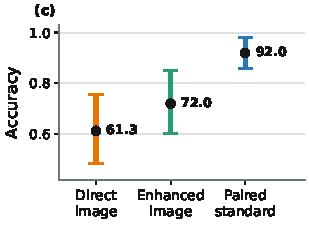
\includegraphics[width=\linewidth]{plots/plot78c_bootstrap_intervals}
\end{subfigure}
\caption{Diagnostic evidence on the locked 75-crop support: (a) score gains,
(b) image-expert progression, and (c) grouped bootstrap intervals. Visual gains
are concentrated rather than uniform.}
\label{fig:score_diagnostics}
\end{figure*}
\fi
%%TRIM-END%%

%%TRIM-BEGIN%% restore by deleting this line and the matching TRIM-END
\iffalse
\begin{figure*}[t]
\centering
\begin{subfigure}[b]{0.1966\textwidth}
  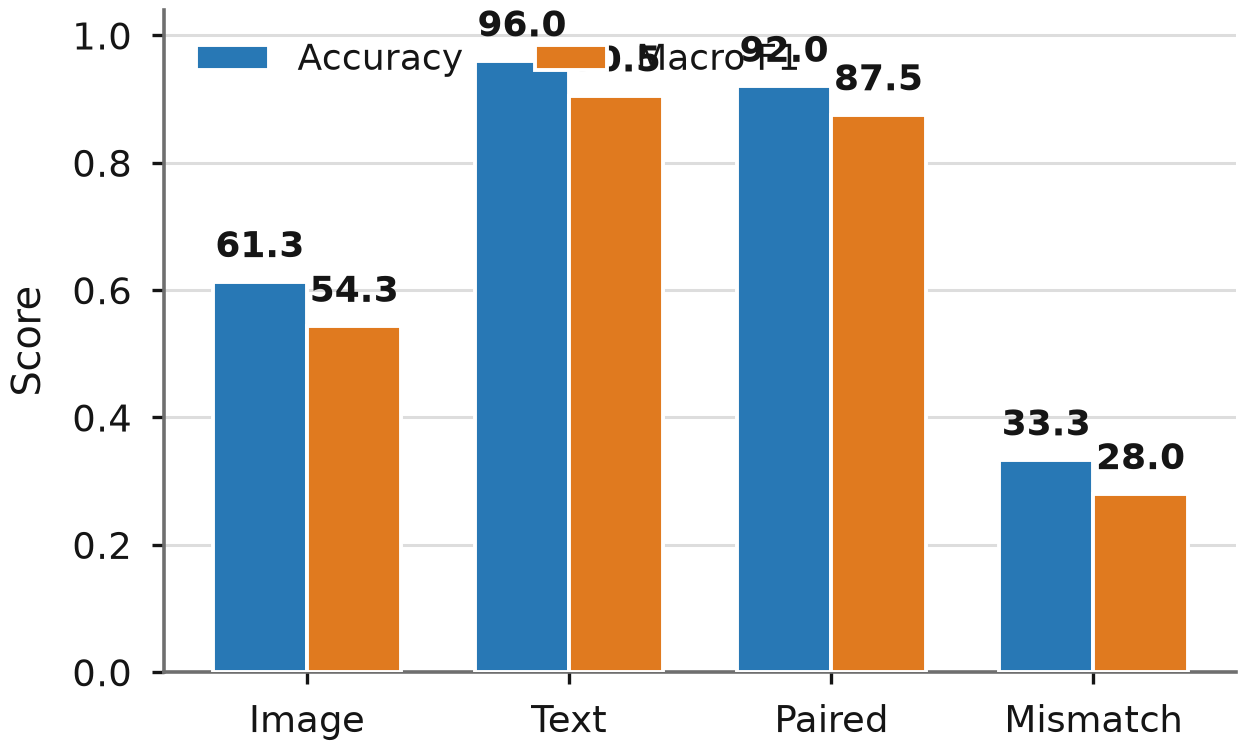
\includegraphics[width=\linewidth]{plots/plot65_standard_multimodal_ablation}
  \caption{Controlled paired-input ablation.}
\end{subfigure}\hfill
\begin{subfigure}[b]{0.1966\textwidth}
  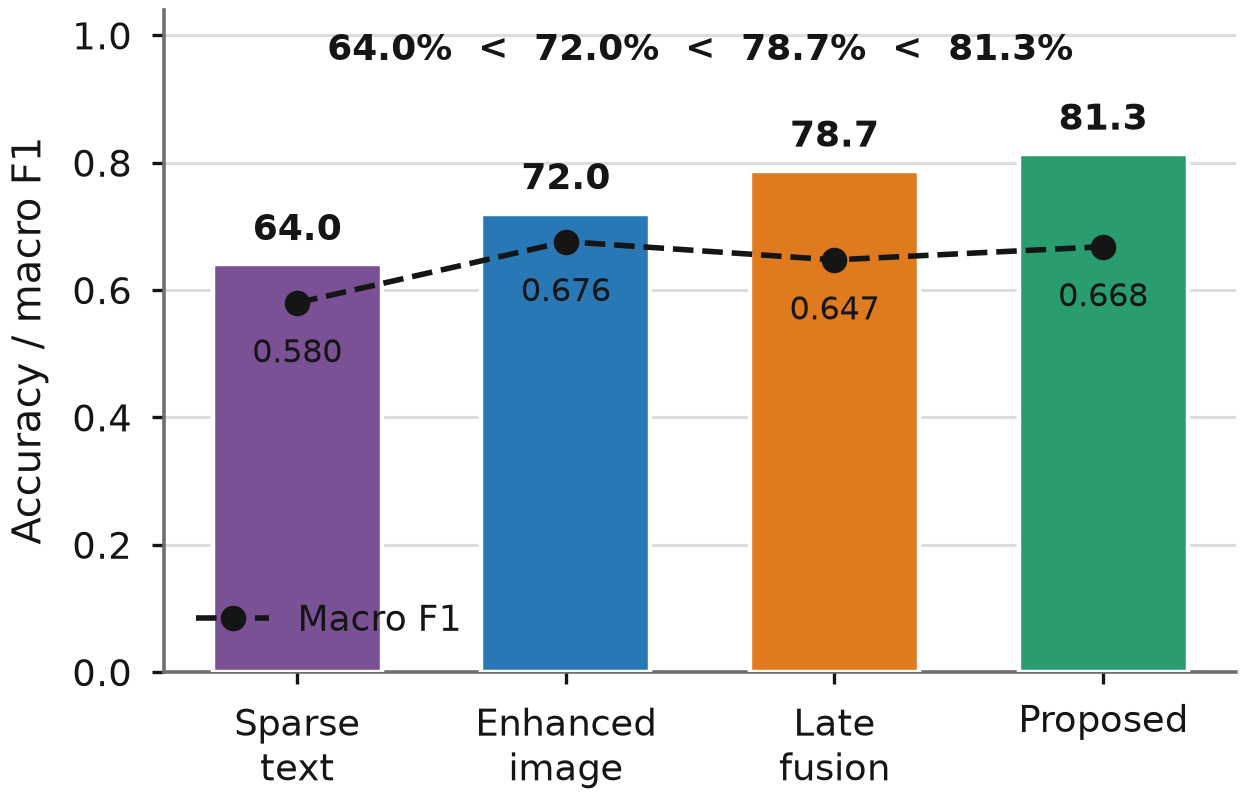
\includegraphics[width=\linewidth]{plots/plot66_sparse_field_note_hierarchy}
  \caption{Sparse-note routing hierarchy.}
\end{subfigure}\hfill
\begin{subfigure}[b]{0.1966\textwidth}
  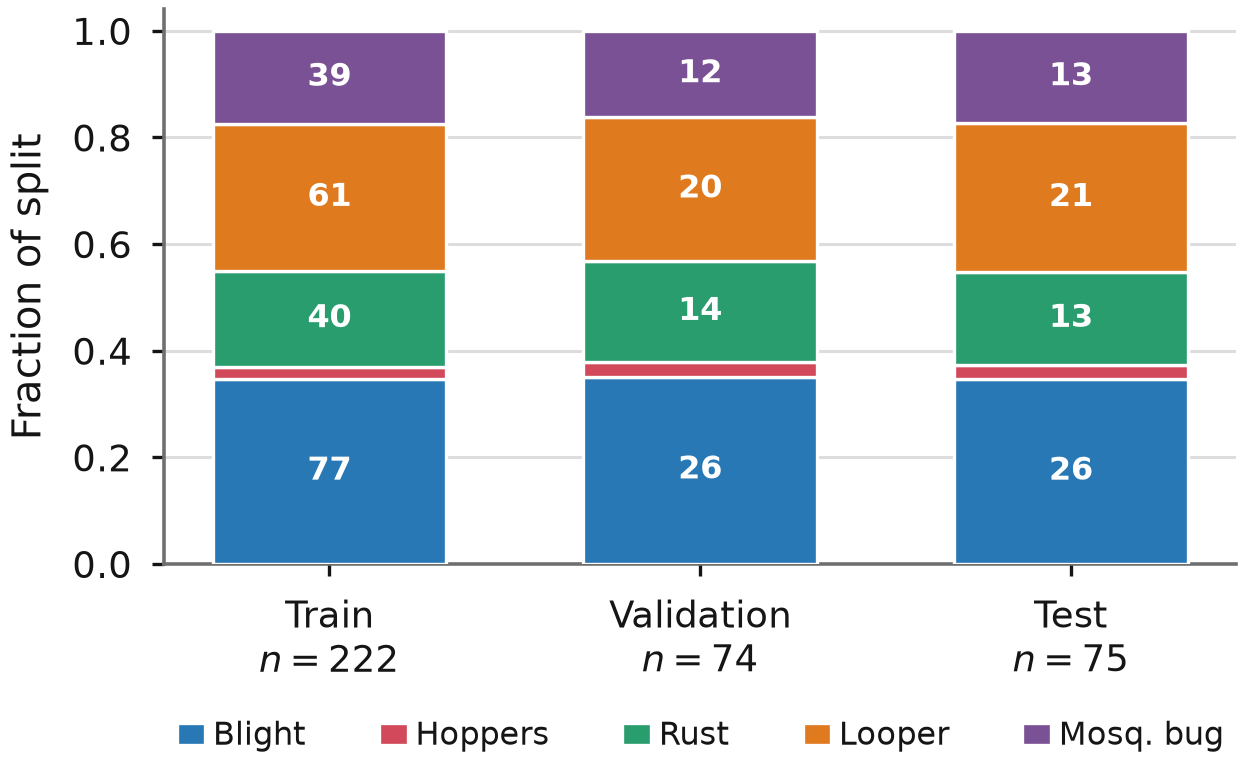
\includegraphics[width=\linewidth]{plots/plot69_dataset_split_audit}
  \caption{Grouped split class balance.}
\end{subfigure}\hfill
\begin{subfigure}[b]{0.1966\textwidth}
  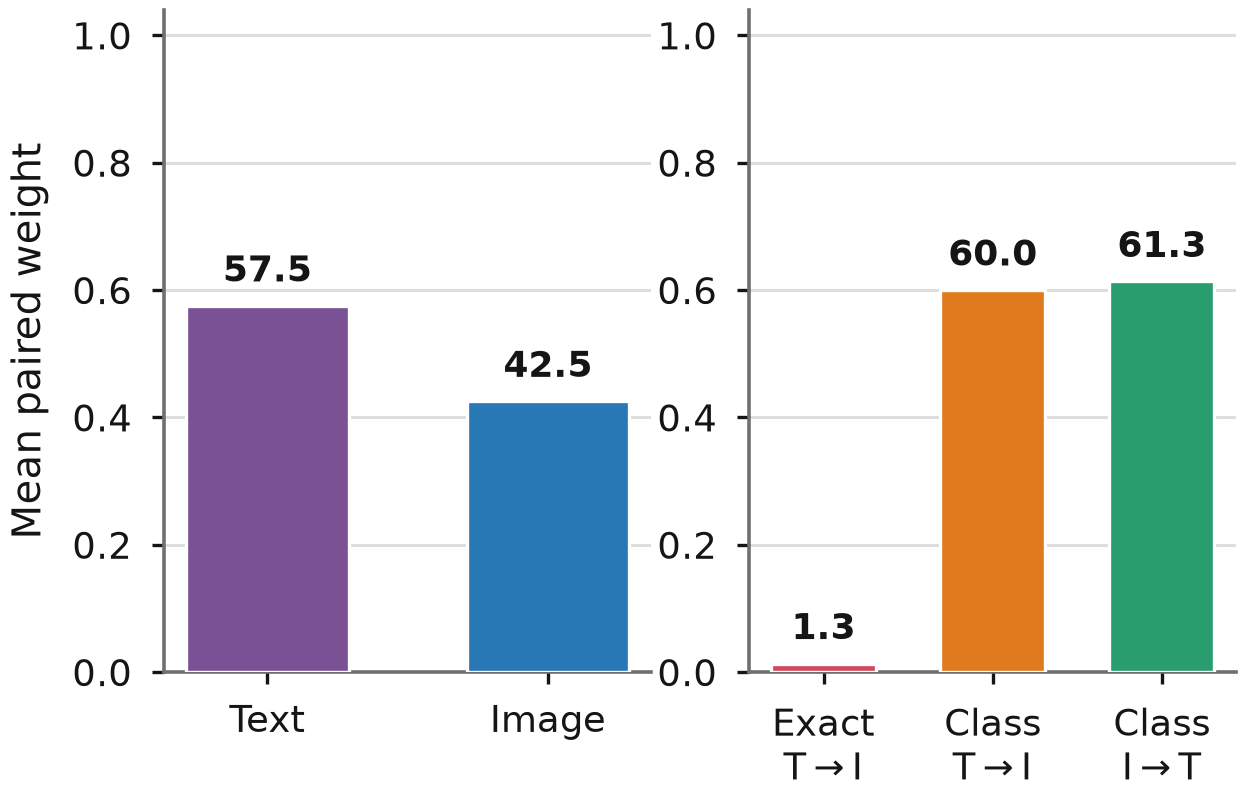
\includegraphics[width=\linewidth]{plots/plot71_crossmodal_diagnostics}
  \caption{Reliability and retrieval probes.}
\end{subfigure}
\caption{Compact diagnostic panels. (a) and (c) are controlled audited data;
(b) is exploratory; (d) distinguishes class-level alignment from exact-pair
retrieval. Metrics with different supports are not pooled.}
\label{fig:compact_diagnostics}
\end{figure*}
\fi
%%TRIM-END%%

\subsection{Advisory Retrieval Results}
\label{sec:advisory_eval}
\label{sec:advisory_results}

%%TRIM-BEGIN%% restore by deleting this line and the matching TRIM-END
\iffalse
\begin{figure*}[t]
\centering
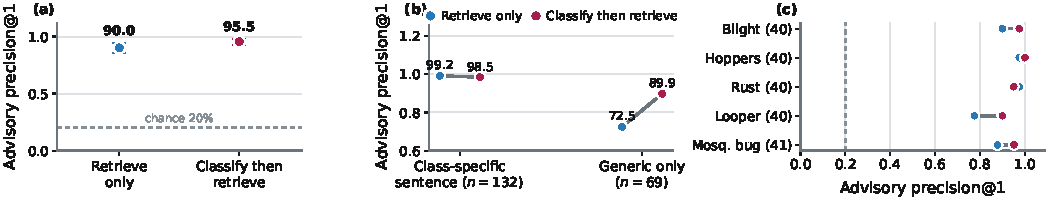
\includegraphics[width=0.5200\textwidth]{plots/plot80_advisory_retrieval}
\caption{Measured Classify--Retrieve--Advise quality on the templated symptom
corpus: 472 passages, 201 queries, exact inner-product search. (a) Precision@1
with bootstrap intervals against chance; (b) split by whether the query holds a
class-unique sentence; (c) per class. Same five classes as the diagnostic
experiments, but a different corpus and support, never pooled with them.}
\label{fig:advisory}
\end{figure*}
\fi
%%TRIM-END%%

Retrieval reaches 90.05\% correct-class
precision@1 against a 20.01\% chance rate, rising to 95.52\% with the classify
stage. That second number \emph{is} the classifier's accuracy, because retrieval
restricted to one predicted class can only return that class, so routing rather
than ranking decides correctness. A stratified query audit locates the failure:
open retrieval
is near-saturated (99.24\%) on the queries carrying a class-unique sentence and
falls to 72.46\% on the rest, which routing lifts to 89.86\%. Figure~\ref{fig:c_retrieval_heatmap} shows where the misses go: looper
caterpillars is the weak row, losing queries to blight, rust and mosquito
bug, whose damage vocabulary it shares.

Three limits apply. The corpus is template-composed, so base and queries share
sentence vocabulary even though no observation is shared, and these are upper
bounds relative to free-form notes. The fusion re-ranker, the OBB overlay and
the agronomic correctness of the advice remain unevaluated: this is a retrieval
result, not evidence that the treatment is right.

%%TRIM-BEGIN%% restore by deleting this line and the matching TRIM-END
\iffalse
\begin{figure}[t]
\centering

\includegraphics[width=\linewidth]{plots/plot89_retrieval_boxplot}
\caption{Top-1 retrieval similarity per tea class, split by whether that top-1 hit was the correct class. The two distributions overlap almost entirely and on mosquito bug the wrong hits score higher, so cosine similarity does not separate a correct advisory from an incorrect one on this corpus: the score is uniformly high because the notes are template-composed. Wrong-hit boxes are drawn from as few as one query for hoppers and rust, so their spread is not informative.}
\label{fig:retrieval_box}
\end{figure}
\fi
%%TRIM-END%%

%%COMPACT-BEGIN%%
\begin{figure}[t]
\centering

\includegraphics[width=\figw]{plots/c21_retrieval_heatmap}
\caption{Advisory retrieval confusion: true class against top-1 retrieved class, row-normalized so the diagonal is per-class precision@1; cells are query counts. Looper caterpillars is the weak row (31/40); hoppers and rust retrieve almost perfectly.}
\label{fig:c_retrieval_heatmap}
\end{figure}
%%COMPACT-END%%


%%TRIM-BEGIN%% restore by deleting this line and the matching TRIM-END
\iffalse
\begin{table}[H]
\centering
\caption{Reproducibility manifest for the updated run}
\label{tab:manifest}
\scriptsize
\setlength{\tabcolsep}{3.2pt}
\begin{tabular}{p{0.36\columnwidth}p{0.31\columnwidth}p{0.24\columnwidth}}
\toprule
Control & Recorded value & Status \\
\midrule
Source split & seed 42; 122/40/38 sources & fixed \\
Cross-split overlap & 0 source photographs & verified \\
Crop--text pairing & 371/371 exact box keys & verified \\
Shortcut vocabulary & 178 tokens; train fitted & fixed \\
Checkpoint reload & strict key match & passed \\
Architecture ablation & 9 variants; CPU/H100 reruns & single seed each \\
DistilBERT selection & 90 candidates; validation only & fixed before test embed. \\
ViT+PLM VLM screen & 360 candidates; validation accuracy & incumbent retained \\
Visual gate search & 3,125 gates on validation & completed \\
Internal test support & 75 crops / 38 sources & common \\
FedAvg adaptation & $K=2,3,5,8$; 8 rounds & completed \\
FL repetitions & seeds 42/123/2026 & partition seeds \\
FL evaluation & 74 validation crops & test untouched \\
Matched proxy suite & 1{,}000 pairs; 700/150/150 split & label-matched proxy \\
Matched FL baselines & 4 aggregators + local-only & completed; no errors \\
\bottomrule
\end{tabular}
\end{table}
\fi
%%TRIM-END%%


%%TRIM-BEGIN%% restore by deleting this line and the matching TRIM-END
\iffalse
\begin{figure*}[t]
\centering
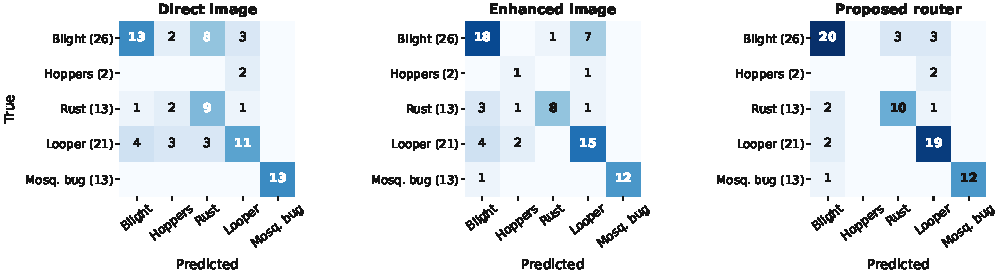
\includegraphics[width=0.7367\textwidth]{plots/plot79_confusion_matrices}
\caption{Where the errors land on the fixed 75-crop test. Each matrix sums to
75; diagonals give the 46, 54, and 61 correct crops of the direct image path,
the five-expert enhanced gate, and the exploratory router. All panels share one
count colour scale, so shading is directly comparable. The off-diagonal
cells are the part no count table records: leaf blight is confused with rust and
looper rather than scattered, looper recovers most under the router, and the two
leaf-hopper crops fall into looper except for one the enhanced gate recovers.}
\label{fig:confusion}
\end{figure*}
\fi
%%TRIM-END%%

\subsection{Reproducibility and Threats to Validity}

The released bundle records data identity, checkpoint state, every federated
round and each realized client partition; deterministic grouping, strict reload
and validation-only adaptation are reproducible, but external estate transfer is
not inferred from them. The locked test is small (38 sources, 75 crops, two leaf-hopper crops), and
selection on 74 validation crops can overfit. The central checkpoint has one
seed; FL seeds vary only client partitions, and clients are simulated.
DistilBERT is a PLM rather than a generative LLM. The corruption probe is one
seeded realization per severity and carries no interval. The robustness sweep
federates linear probes on frozen features, so its invariances belong to that
estimator and not to the deep model. Deployment requires multi-estate data,
independent notes, rare-class coverage, and repeated end-to-end training.

% The previous proxy-pair evaluation is retained below as inactive source
% history; it is excluded from the compiled manuscript.
\iffalse
\section{Performance Evaluation}
\label{sec:eval_old}

\subsection{Setup and Protocol}

Experiments run on a Tesla T4 using PyTorch with mixed
precision. Both branches use AdamW (weight decay 0.01, batch 16, warmup then
cosine decay, clipping 1.0). The \textbf{text branch} peaks at $2\times10^{-5}$
over 12 epochs (patience 6). The \textbf{vision branch} peaks at $10^{-4}$ over
at most 15 epochs and unfreezes progressively --- head alone for 1 epoch, final
encoder stage at epoch 2, full encoder at epoch 4, each group's LR clock starting
on activation --- which on 139 images is what prevents early gradients from
destroying pretrained features; it also selects per epoch between original-only
inference and a horizontal-flip feature mean.

Three rules govern every number. \textbf{(i) Selection uses validation only},
scored at group level (10 text template groups, 30 vision source groups); test
never participates. \textbf{(ii) Reporting is on a common support}: all modality
conditions and centralized/federated pairs are scored on the identical 30
held-out pairs with asserted identical label order, so paired tests are valid.
\textbf{(iii) Uncertainty is scoped}: Wilson intervals for proportions, paired
class-stratified percentile bootstrap (2\,000 replicates) for macro-F1
differences, conditional on one fitted checkpoint --- \emph{not} training-seed
uncertainty. Macro F1 is primary because the test support is imbalanced (10
blight, 1 hopper, 5 rust, 7 looper, 7 mosquito).

\subsection{Encoder Baselines: Why Each Score Lands Where It Does}
\label{sec:encoders}

\begin{table}[t]
\caption{Encoder Performance. Text is scored on 15 independent template groups; vision on 30 source-disjoint photographs. Group-level accuracy resolves only in steps of $1/15$, which is why three text encoders share $11/15$; the row-level macro F1 ($n{=}189$) separates them. Group-level remains primary, since rows within a template family are near-duplicates and row-level weighting over-counts prolific templates.}
\label{tab:encoders}
\centering\footnotesize
\setlength\tabcolsep{2.6pt}
\begin{tabular}{lccccc}
\toprule
\textbf{Encoder} & \textbf{Params} & \textbf{Val} & \textbf{Corr.} & \textbf{Test F1 (95\% CI)} & \textbf{Macro}\\
\midrule
\multicolumn{6}{l}{\textit{Text: 15 template groups (Macro $=$ group\,/\,row-level, $n{=}189$)}}\\
BERT-tiny     & 4.4M  & 0.587 & 11/15 & 0.733 (0.480--0.891) & 0.717 / 0.550 \\
BERT-mini     & 11.2M & 0.706 & 11/15 & 0.733 (0.480--0.891) & 0.723 / 0.597 \\
BERT-small    & 28.8M & 0.762 & 11/15 & 0.733 (0.480--0.891) & 0.741 / 0.665 \\
\textbf{BERT-medium} & 41.4M & 0.960 & 13/15 & \textbf{0.867 (0.621--0.963)} & \textbf{0.863 / 0.808} \\
DistilBERT    & 66.4M & 0.929 & 13/15 & 0.867 (0.621--0.963) & 0.867 / 0.830 \\
\midrule
\multicolumn{6}{l}{\textit{Vision}}\\
EfficientNet-B0 & 4.0M  & 0.667 & 20/30 & 0.667 (0.488--0.808) & 0.557 \\
DeiT-tiny       & 5.6M  & 0.733 & 21/30 & 0.700 (0.521--0.833) & 0.598 \\
Swin-tiny       & 27.5M & \textbf{0.800} & 19/30 & 0.633 (0.455--0.781) & 0.503 \\
ConvNeXT-tiny   & 27.8M & \textbf{0.800} & 23/30 & \textbf{0.767 (0.591--0.882)} & \textbf{0.640} \\
ViT-Base        & 86.4M & 0.767 & 22/30 & 0.733 (0.556--0.858) & 0.602 \\
\bottomrule
\end{tabular}
\end{table}

\begin{figure*}[!tb]
  \centering
  \begin{subfigure}[b]{0.298\textwidth}
    
\includegraphics[width=\linewidth]{plots/plot01_llm_comparison}
    \caption{Text encoders (group-level).}
    \label{fig:llmcomp}
  \end{subfigure}\hfill
  \begin{subfigure}[b]{0.298\textwidth}
    
\includegraphics[width=\linewidth]{plots/plot02_vit_comparison}
    \caption{Vision backbones.}
    \label{fig:vitcomp}
  \end{subfigure}\hfill
  \begin{subfigure}[b]{0.298\textwidth}
    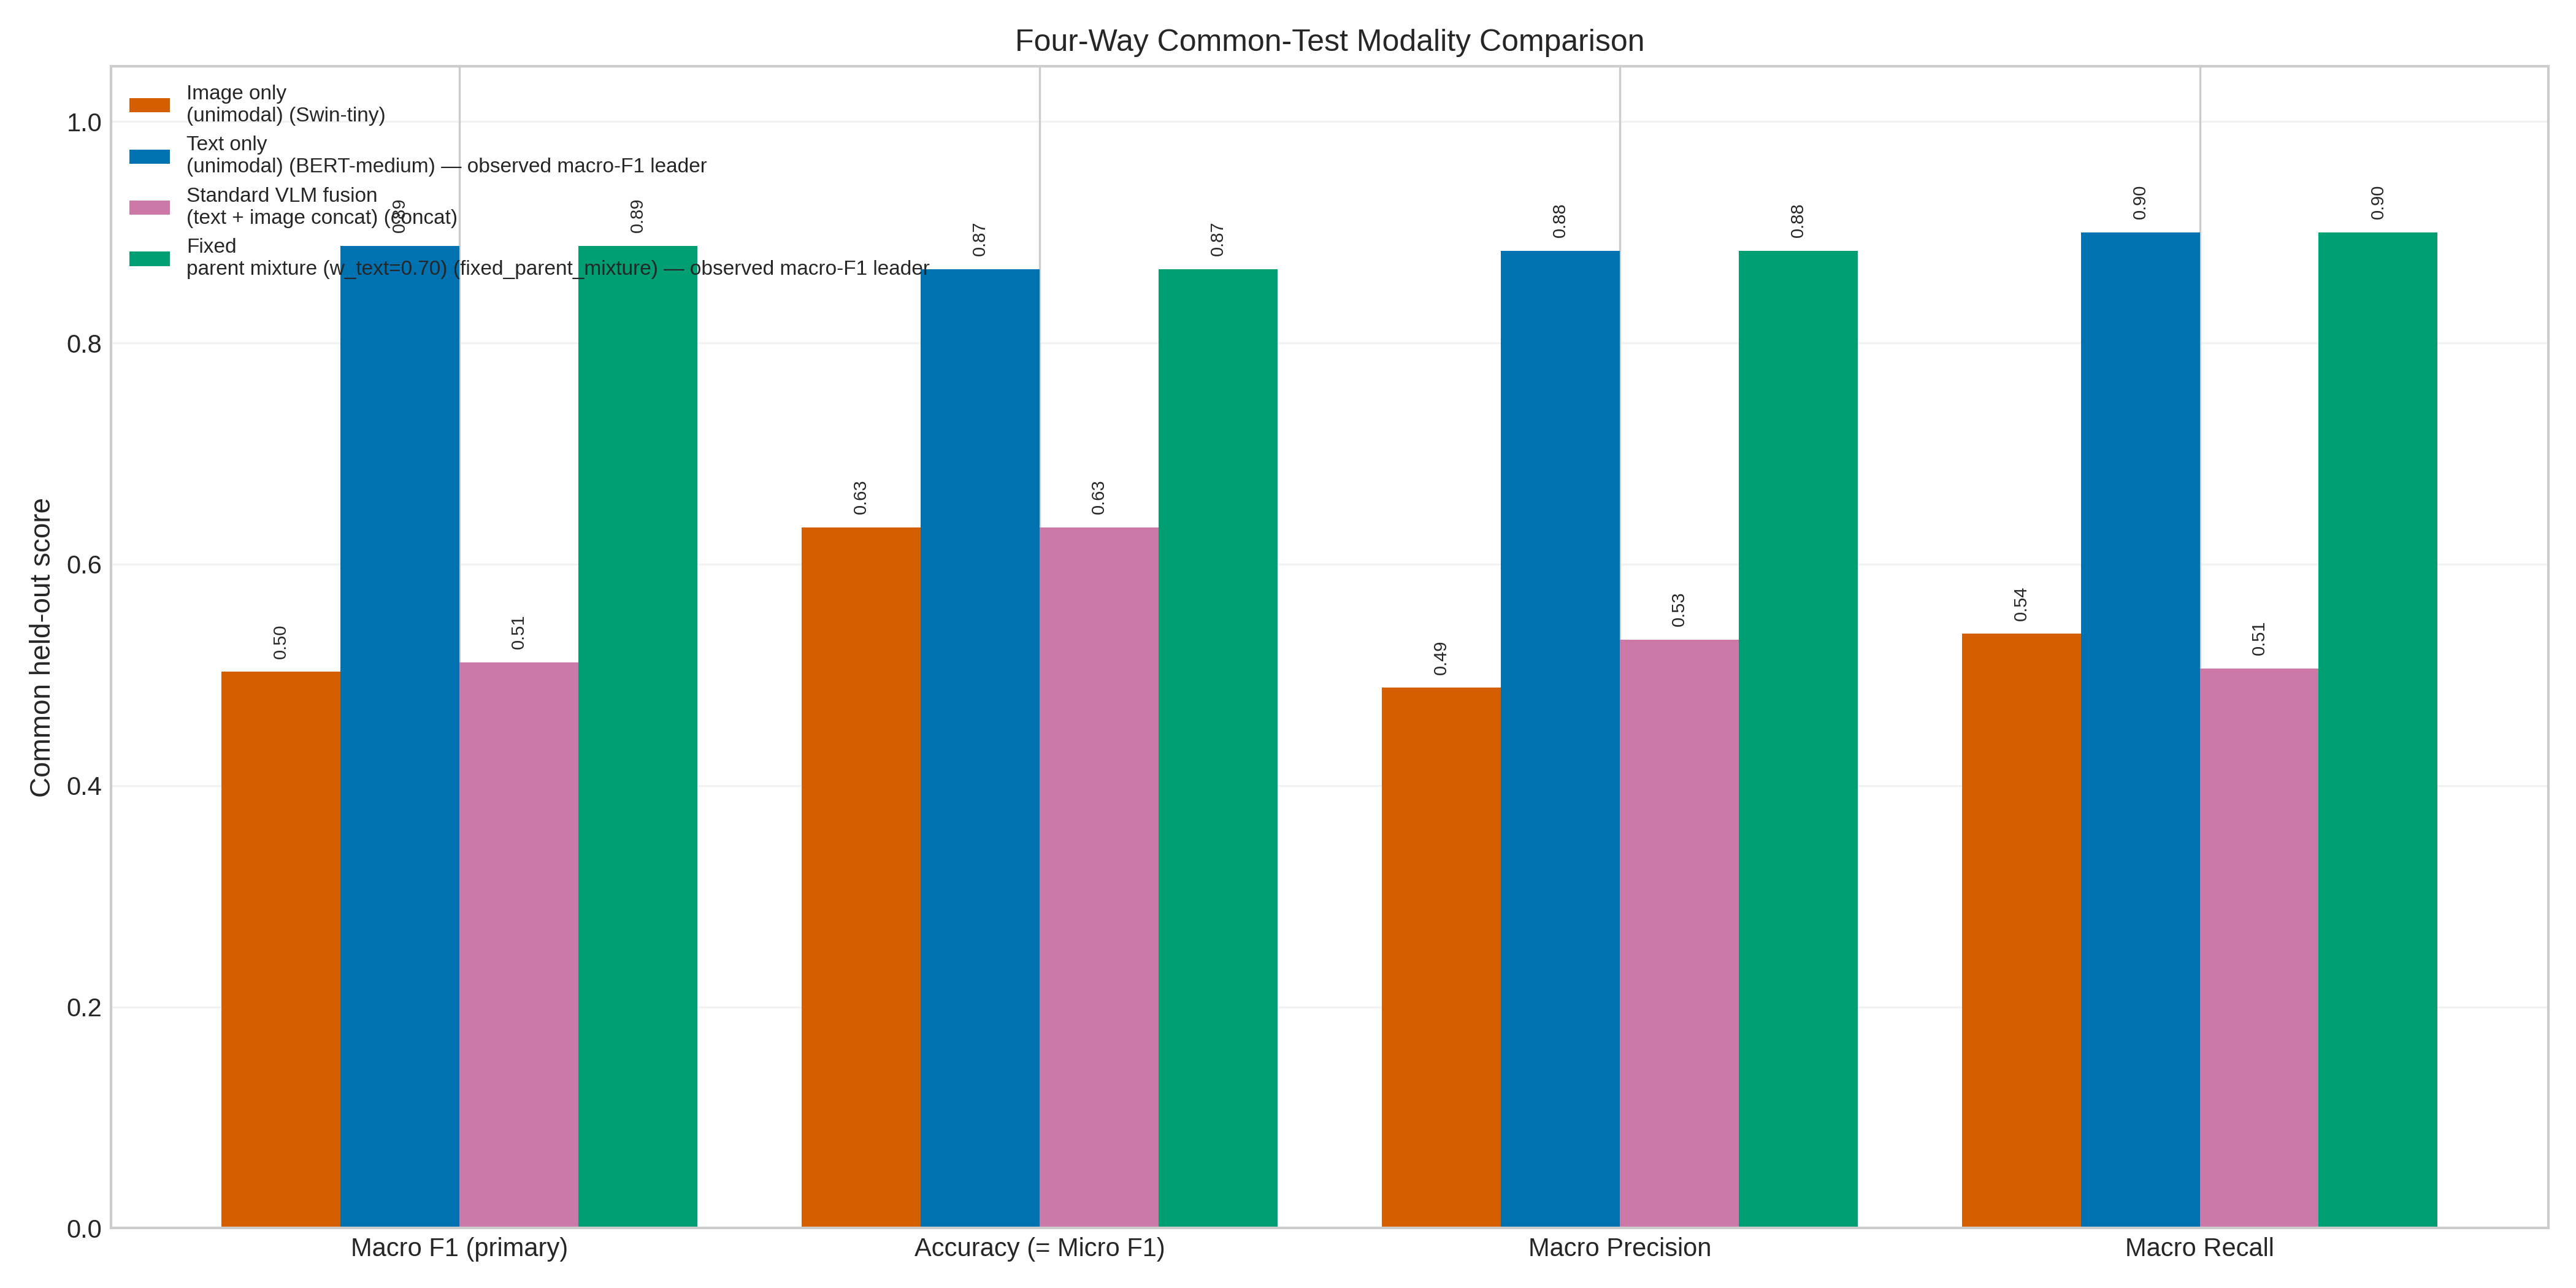
\includegraphics[width=\linewidth]{plots/plot10d_four_way_modality_comparison}
    \caption{Four-way modality comparison.}
    \label{fig:fourwayfig}
  \end{subfigure}
  \caption{Encoder baselines and the four-way comparison. Text macro F1 tracks accuracy closely (a), but vision macro F1 sits well below its accuracy at every backbone (b) --- the signature of a class scoring zero, here the 6-training-photo leaf-hoppers class. In (c) the two multimodal-capable conditions bracket the outcome: concatenation lands at the image-only level, the gated model at the text-only level, and neither sits above both parents.}
  \label{fig:encoders}
\end{figure*}

Table~\ref{tab:encoders} and Figure~\ref{fig:encoders} report both branches.
Three drivers explain the pattern.

\textbf{Why text is high (0.863--0.867).} The corpus is authored from 55 templates
with class-structured vocabulary. Even after group-disjoint splitting removes
surface-form memorisation, held-out templates of a class still share the
diagnostic terms that define it, so a pretrained encoder transfers well.
Performance scales monotonically with capacity, 0.717 at 4.4M to 0.867 at 66.4M.
The caveat is that this is an unlinked benchmark: 0.867 measures separability of
authored descriptions, not of field notes.

\textbf{Why vision is low (0.503--0.640).} Three compounding causes. (i)
\emph{Data volume}: 139 independent training photographs for backbones of 4--86M
parameters. Capacity does not help --- the 86.4M ViT-Base does not beat the 27.8M
ConvNeXT-tiny. (ii) \emph{Extreme minority classes}: 6 training photographs for
leaf-hoppers, on which the fed-matched control scores 0.0 F1 in both arms,
dragging the five-class macro average down by up to 0.2 relative to micro F1.
(iii) \emph{Fine-grained visual similarity}: blight necrosis and rust pustules
are both brown lesions on cluttered field backgrounds, and the confusions in
Section~\ref{sec:headroom} are concentrated exactly there.

\textbf{A selection failure worth reporting.} Swin-tiny and ConvNeXT-tiny tie
exactly at 0.800 validation, yet differ by 0.137 macro F1 on test (19/30 vs.\
23/30). Swin-tiny was chosen as vision parent by the tie-break and is the weaker.
With 30 validation images a tie carries almost no information. We report the
consequence rather than silently re-running: the proposed model is built on the
weaker branch. All five intervals in each block overlap; the orderings are
suggestive, not established.

\subsection{Fusion Results: Why Scratch Fusion Fails}

\begin{figure}[t]
  \centering
  
\includegraphics[width=0.94\columnwidth]{plots/plot03_vlm_fusion_comparison}
  \caption{All ten fusion variants on the common test support. The eight scratch surrogates (left) occupy a band from 0.261 to 0.610 macro F1 --- every one of them below the 0.867 a pretrained text encoder reaches \emph{alone} --- while the two pretrained-parent models (right) sit at 0.888. The separation is a statement about pretraining, not about fusion design.}
  \label{fig:fusioncomp}
\end{figure}

\begin{table}[t]
\caption{Fusion Strategies on the Common Test Support ($n{=}30$)}
\label{tab:vlmres}
\centering\footnotesize
\setlength\tabcolsep{3pt}
\begin{tabular}{lcccc}
\toprule
\textbf{Fusion} & \textbf{Params} & \textbf{Val F1} & \textbf{Test F1} & \textbf{Macro F1}\\
\midrule
\multicolumn{5}{l}{\textit{Pooled-feature scratch surrogates}}\\
\quad Unified-IO / Flamingo & 16--17M & 0.30/0.47 & 0.37/0.47 & 0.261 / 0.309\\
\quad Cross-Attn / Gated    & 15.8M & 0.37 & 0.57/0.60 & 0.429 / 0.447\\
\quad CLIP / BLIP-2         & 15.8M & 0.40 & 0.60/0.63 & 0.461 / 0.509\\
\quad Concatenation         & 15.6M & 0.367 & 0.633 & 0.511\\
\quad CoCa                  & 16.2M & 0.400 & 0.733 & 0.610\\
\midrule
\multicolumn{5}{l}{\textit{Pretrained-parent models}}\\
\quad Late fusion (frozen)  & 68.9M & 1.000 & 0.867 & 0.888\\
\rowcolor{vlmred!30}
\quad \textbf{Proposed gated} & 70.1M & \textbf{1.000} & \textbf{0.867} & \textbf{0.888}\\
\bottomrule
\end{tabular}
\end{table}

The gap between the two blocks of Table~\ref{tab:vlmres} and
Figure~\ref{fig:fusioncomp} is a statement about
\emph{pretraining}, not fusion. Every scratch surrogate trained on 139 image
groups and 30 text groups lands between 0.261 and 0.610 --- all below the 0.867
a pretrained text encoder achieves alone. At this scale a fusion operator cannot
be learned from scratch over pooled features, and reporting such a surrogate as a
``CLIP-style'' result would misrepresent what those architectures do when properly
pretrained. We report them as scale-calibrated baselines. Both pretrained-parent
models reach 0.888 and both saturate validation at 1.000, which on 30 pairs is an
artefact, not headroom --- and is why validation could not discriminate among gate
modes.

\subsection{Four-Way Modality Comparison}
\label{sec:fourway}

\begin{table}[t]
\caption{Four-Way Comparison and Calibration ($n{=}30$, common support)}
\label{tab:fourway}
\centering\footnotesize
\setlength\tabcolsep{2.2pt}
\begin{tabular}{lccccc}
\toprule
\textbf{Condition} & \textbf{Acc.\ (95\% CI)} & \textbf{Macro F1} & \textbf{CI} & \textbf{ECE}$\downarrow$ & \textbf{AURC}$\downarrow$\\
\midrule
Image only      & 0.633 (0.455--0.781) & 0.503 & 0.385--0.624 & \textbf{0.077} & 0.175\\
Text only       & \textbf{0.867 (0.703--0.947)} & \textbf{0.888} & 0.779--0.971 & 0.186 & 0.063\\
Concat fusion   & 0.633 (0.455--0.781) & 0.511 & 0.356--0.637 & 0.131 & 0.317\\
\rowcolor{vlmred!30}
Proposed ($w_t{=}0.70$) & \textbf{0.867 (0.703--0.947)} & \textbf{0.888} & 0.779--0.971 & 0.240 & \textbf{0.038}\\
\bottomrule
\end{tabular}
\end{table}

\begin{figure*}[!tb]
  \centering
  \begin{subfigure}[b]{0.537\textwidth}
    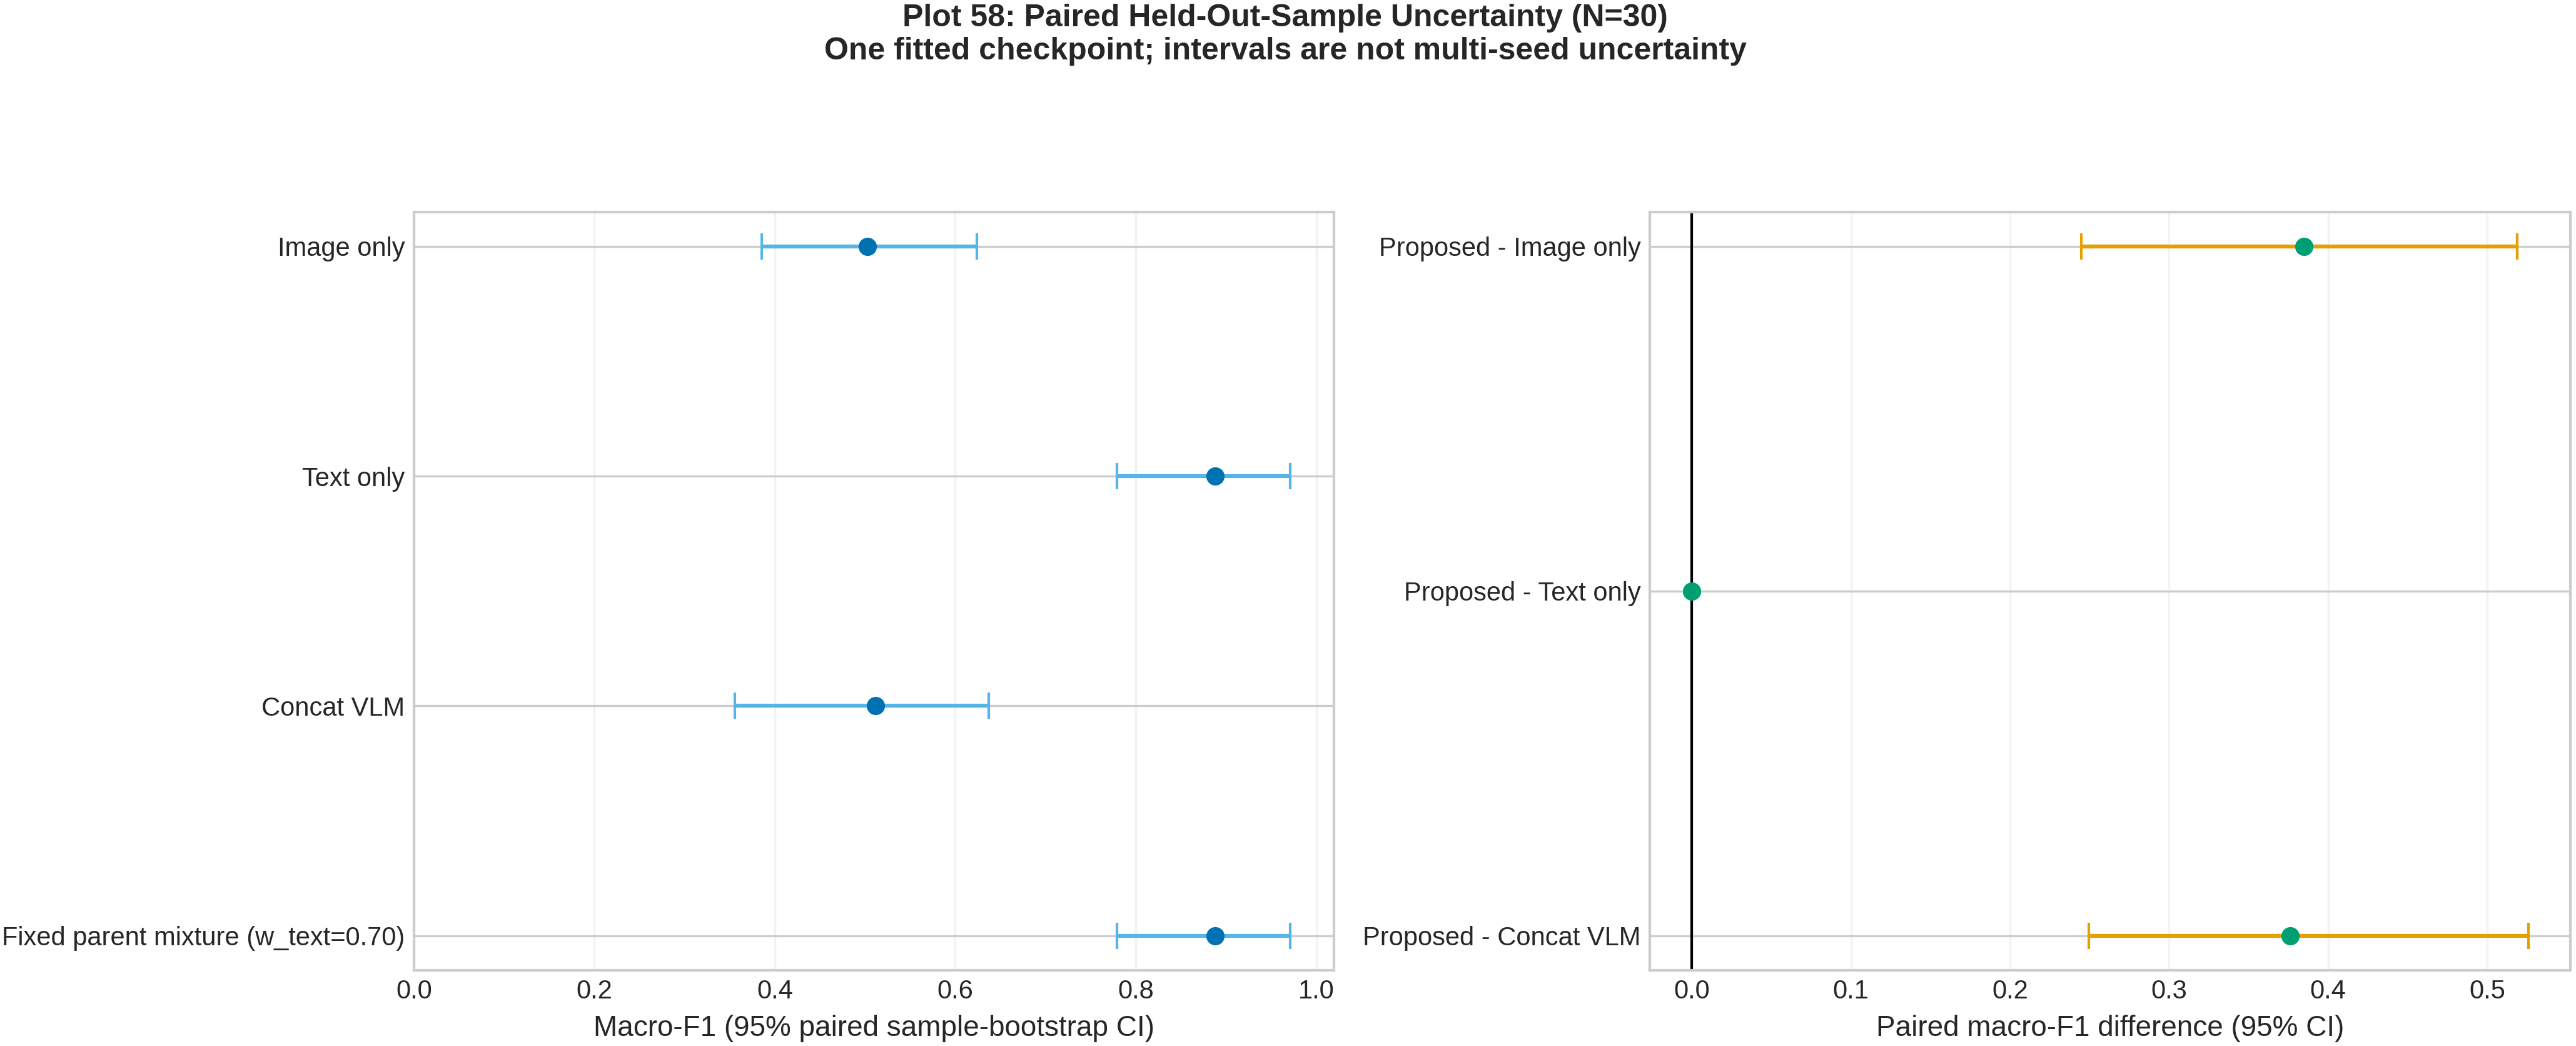
\includegraphics[width=\linewidth]{plots/plot58_paired_bootstrap_ci}
    \caption{Paired class-stratified bootstrap intervals (2\,000 replicates).}
    \label{fig:bootstrap}
  \end{subfigure}%
  \begin{subfigure}[b]{0.276\textwidth}
    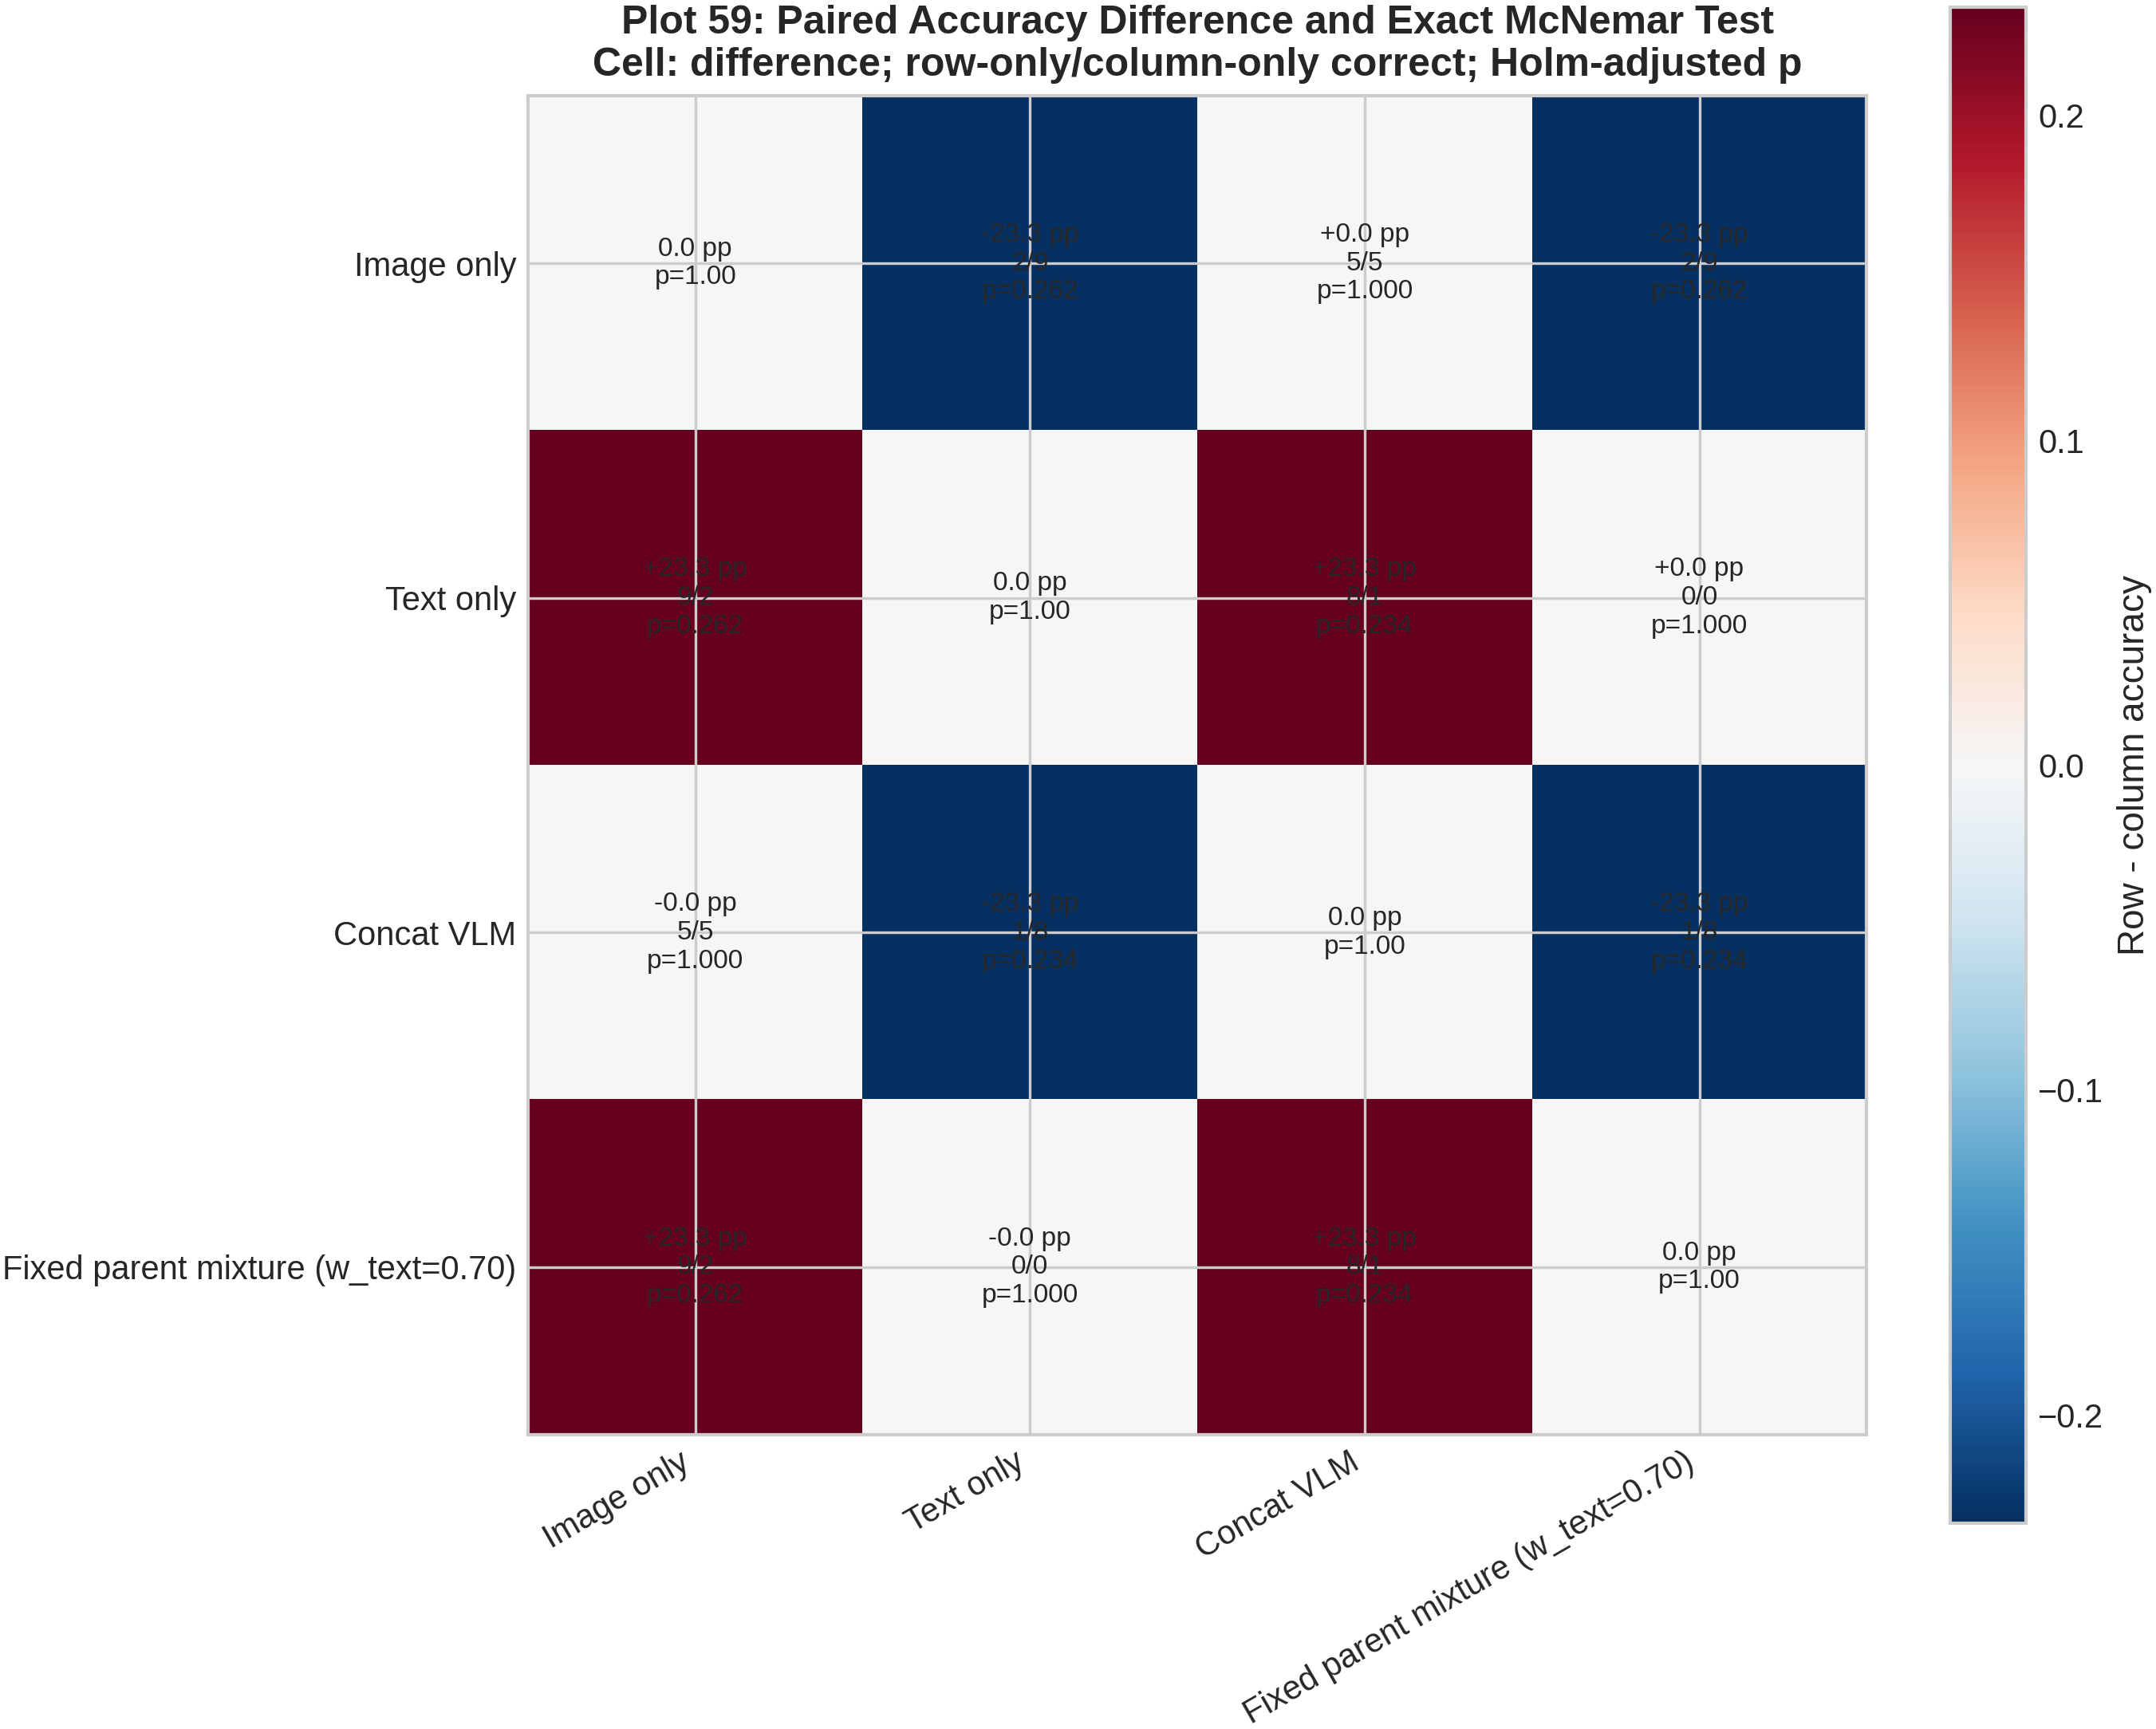
\includegraphics[width=\linewidth]{plots/plot59_mcnemar_matrix}
    \caption{Pairwise exact McNemar discordance, Holm-corrected $p$.}
    \label{fig:mcnemar}
  \end{subfigure}
  \caption{Paired statistics on the common held-out support. The proposed model separates cleanly from image-only and from concatenation fusion, and is indistinguishable from text-only --- zero discordant predictions.}
  \label{fig:paired}
\end{figure*}

Three findings follow from Table~\ref{tab:fourway},
Figure~\ref{fig:fourwayfig}, and Figure~\ref{fig:paired}.

\textbf{(1) Naive fusion underperforms its stronger parent.} Concatenation reaches
0.511 against 0.888 for text alone: adding an image stream \emph{costs} 0.377
macro F1. The paired bootstrap gives $+0.376$ for the pretrained model over
concat (CI 0.250--0.526, bootstrap fraction above zero $1.000$); exact McNemar
gives $p{=}0.039$ uncorrected, $p_{\text{Holm}}{=}0.234$, so the direction is
well-supported and significance is not established at $n{=}30$. Note that concat's
0.511 nearly equals image-only's 0.503 --- it has collapsed onto the image branch.

\textbf{(2) The proposed model matches but does not beat text-only.} The gain over
the strongest baseline is exactly $0.000$; the bootstrap difference is degenerate
at zero and exact McNemar finds \textbf{zero discordant pairs}. The
pre-registered criterion --- macro-F1 leadership with paired accuracy support ---
is \emph{not met}, and the 0.90 accuracy target is met neither at the point
estimate (0.867) nor at the Wilson lower bound (0.703).

\begin{figure*}[!tb]
\centering
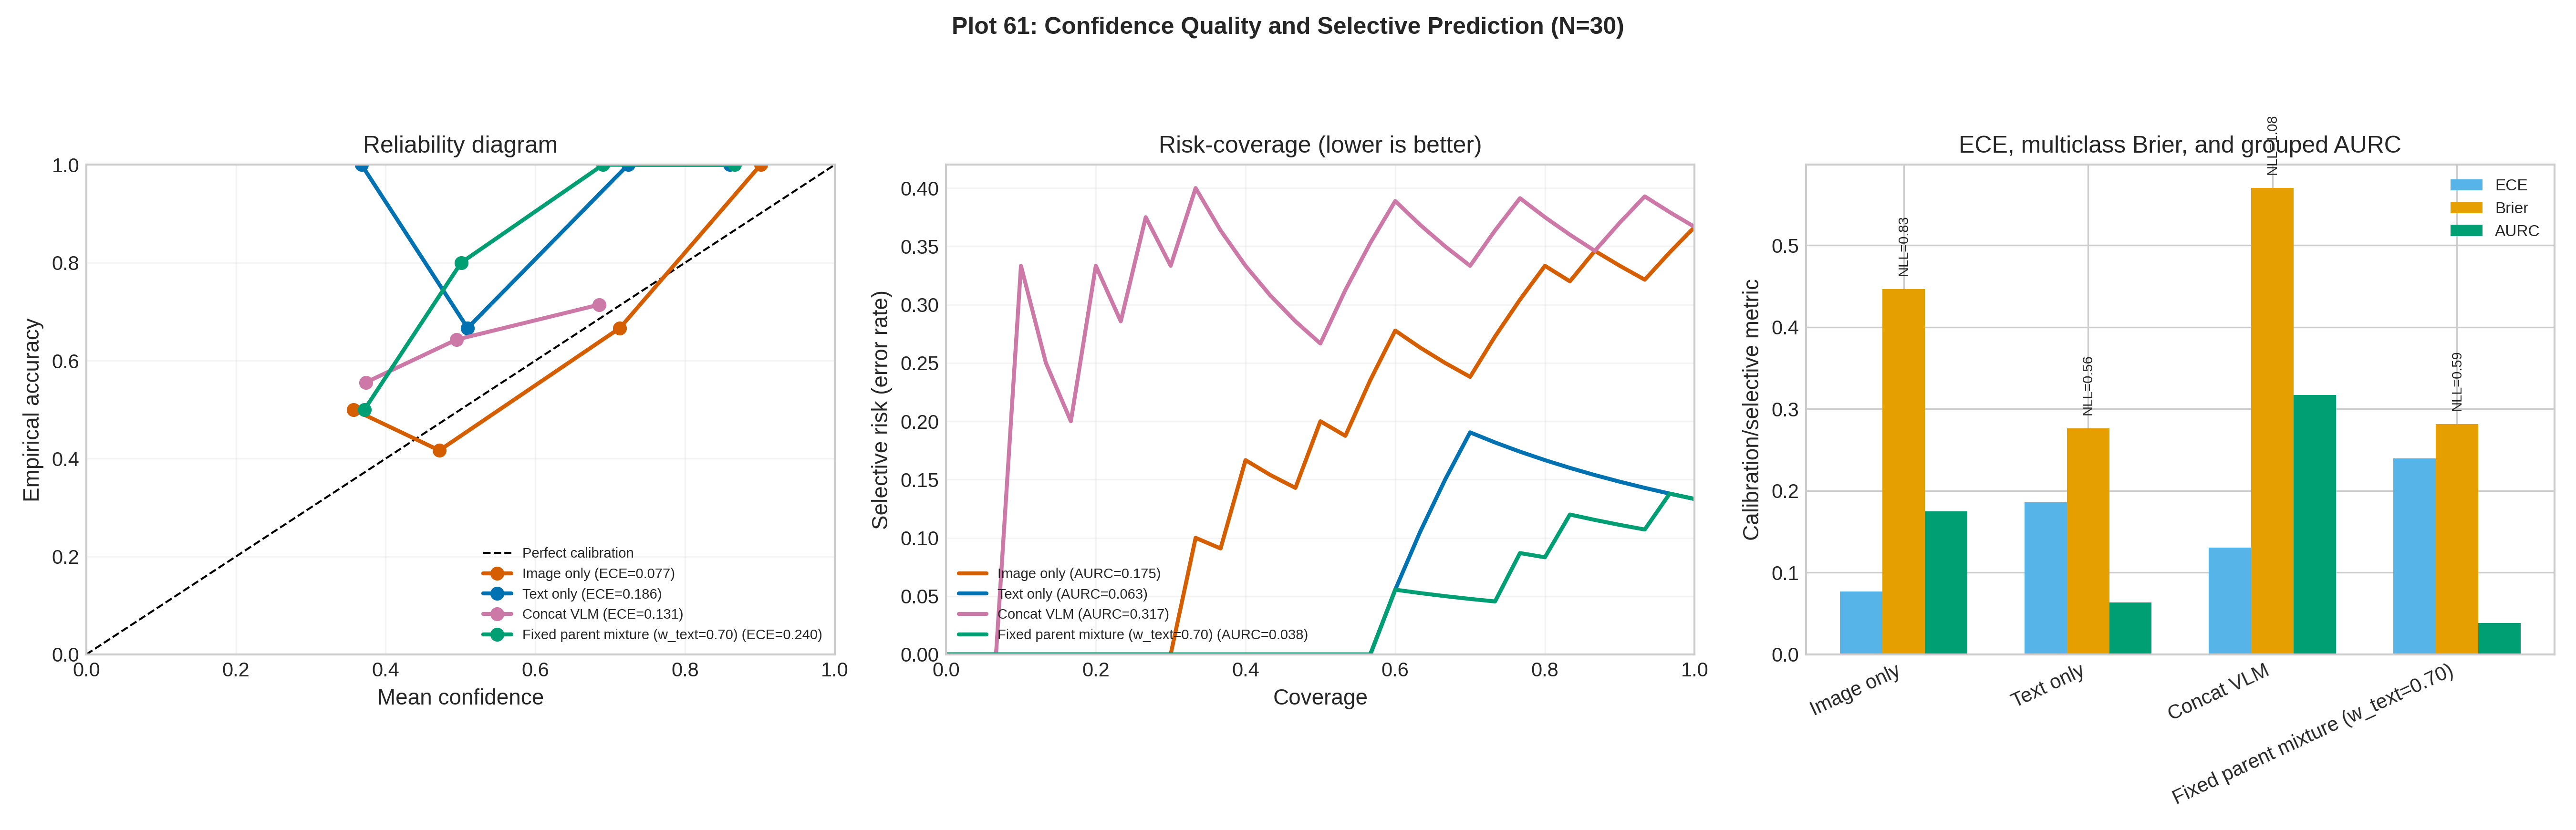
\includegraphics[width=0.777\textwidth]{plots/plot61_calibration_risk_coverage}
\caption{Confidence quality and selective prediction. \textbf{(left)} Reliability: the gated mixture sits furthest above the diagonal, i.e.\ systematically under-confident, which is what its worst-in-table ECE of 0.240 measures. \textbf{(centre)} Risk-coverage: the same model has the \emph{lowest} selective risk at every coverage below 0.6, giving the best AURC (0.038). \textbf{(right)} The three metrics side by side. Under-confidence and good ranking are not in conflict --- which is why an abstention threshold, not a raw probability readout, is the safe deployment mode.}
\label{fig:calib}
\end{figure*}

\textbf{(3) Calibration favours abstention, not raw confidence.} The proposed
model has the worst ECE (0.240) and the best AURC (0.038). These are not in
conflict: mixing at $w_t{=}0.70$ shrinks confidences away from the correct
absolute level, which ECE punishes, while sharpening the \emph{ranking} of correct
over incorrect, which AURC rewards. For a system that escalates to an agronomist
below a threshold, ranking is the operative property; for one reporting raw
probabilities to a farmer, temperature recalibration is required first. Concat
fusion is worst on three of four measures.

\begin{table*}[!tb]
\caption{\textbf{Left:} federated vs.\ centralized macro F1, paired on the same $n{=}30$ support and matched for optimizer, pass budget, and client partition. \textbf{Right:} configuration sweep, final-round global \emph{validation} macro F1 at the low\,/\,high setting of each factor. Sweep values come from the compact matched-budget models and are not comparable to Table~\ref{tab:fourway}.}
\label{tab:fed}
\centering\footnotesize
\setlength\tabcolsep{5pt}
\begin{tabular}{lcccc@{\hskip 20pt}lcccc}
\toprule
\multicolumn{5}{c}{\textbf{Federated vs.\ centralized (paired, test)}} & \multicolumn{5}{c}{\textbf{Configuration sweep (validation, low\,/\,high)}}\\
\cmidrule(lr){1-5}\cmidrule(lr){6-10}
\textbf{Condition} & \textbf{Central} & \textbf{Fed} & \textbf{$\Delta$ (95\% CI)} & \textbf{$p_{\text{Holm}}$} &
\textbf{Factor} & \textbf{ViT} & \textbf{LLM} & \textbf{VLM} & \textbf{s/round}\\
\midrule
Image only    & 0.450 & 0.411 & $-0.039$ ($-0.198$, $0.115$)  & 1.00 & Clients $K$ = 2\,/\,10        & 0.325 / 0.339 & 0.106 / \textbf{0.317} & 0.316 / 0.215 & 3.1--8.8\\
Text only     & 0.139 & 0.139 & $-0.000$ ($-0.060$, $0.072$)  & 1.00 & Local epochs $E$ = 1\,/\,5    & 0.182 / \textbf{0.332} & 0.153 / 0.127 & 0.172 / \textbf{0.337} & 1.8--13.2\\
Concat fusion & 0.438 & 0.248 & $-0.190$ ($-0.332$, $-0.029$) & 1.00 & Participation 0.25\,/\,1.0    & 0.119 / 0.243 & 0.057 / 0.163 & 0.076 / 0.090 & 1.0--8.8\\
Proposed      & 0.314 & 0.230 & $-0.084$ ($-0.219$, $0.052$)  & 1.00 & Dirichlet $\alpha$ 0.1\,/\,10 & 0.384 / \textbf{0.419} & 0.100 / 0.082 & 0.292 / 0.246 & 3.6--8.1\\
\bottomrule
\end{tabular}
\end{table*}

\begin{figure*}[!tb]
  \centering
  \begin{subfigure}[b]{0.222\textwidth}
    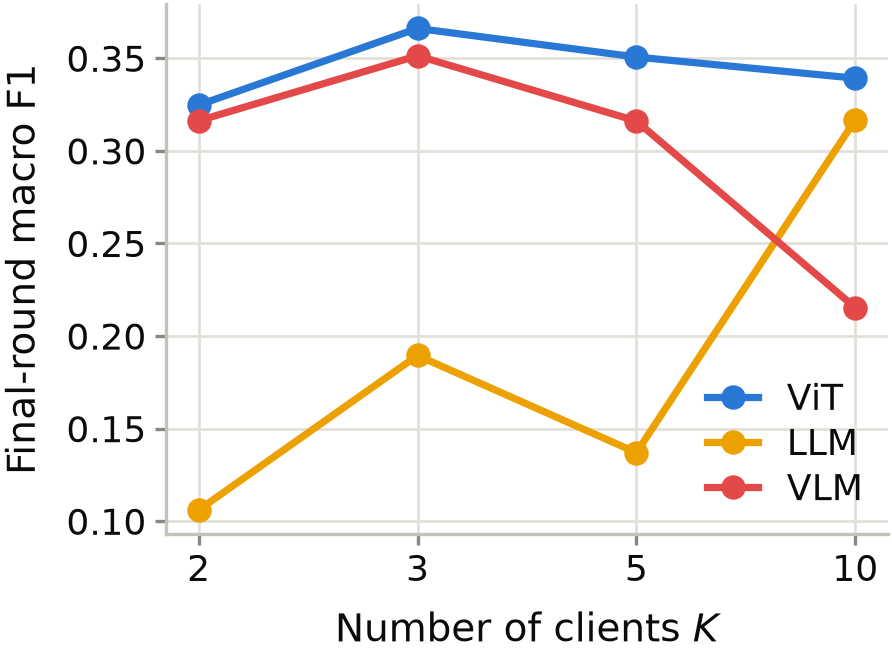
\includegraphics[width=\linewidth]{plots/panels/f10a_clients}
    \caption{Client count: no consistent direction.}
    \label{fig:fedclients}
  \end{subfigure}\hfill
  \begin{subfigure}[b]{0.222\textwidth}
    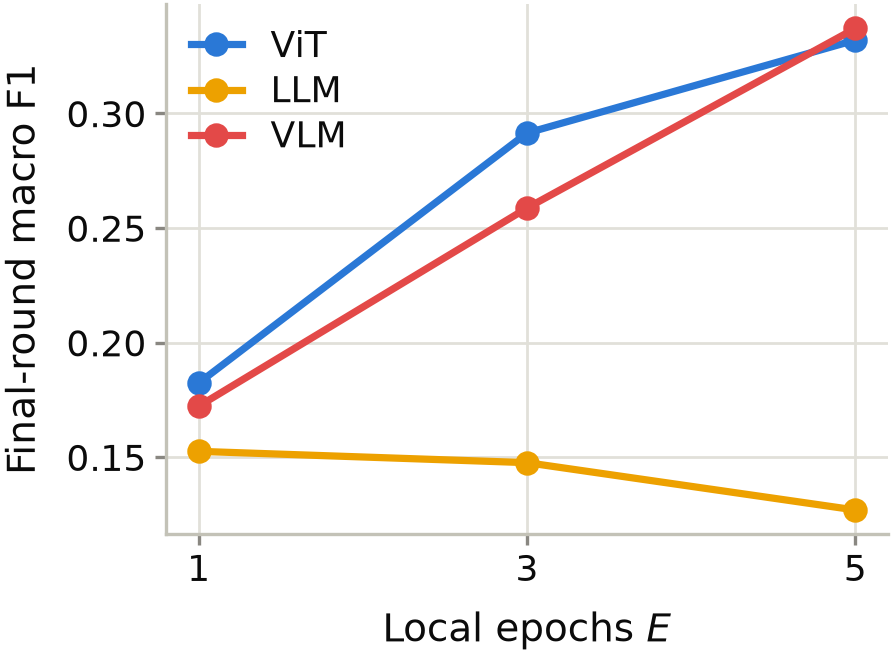
\includegraphics[width=\linewidth]{plots/panels/f10e_epochs}
    \caption{Local epochs $E$: the one monotone effect.}
    \label{fig:sweepfactors}
  \end{subfigure}\hfill
  \begin{subfigure}[b]{0.222\textwidth}
    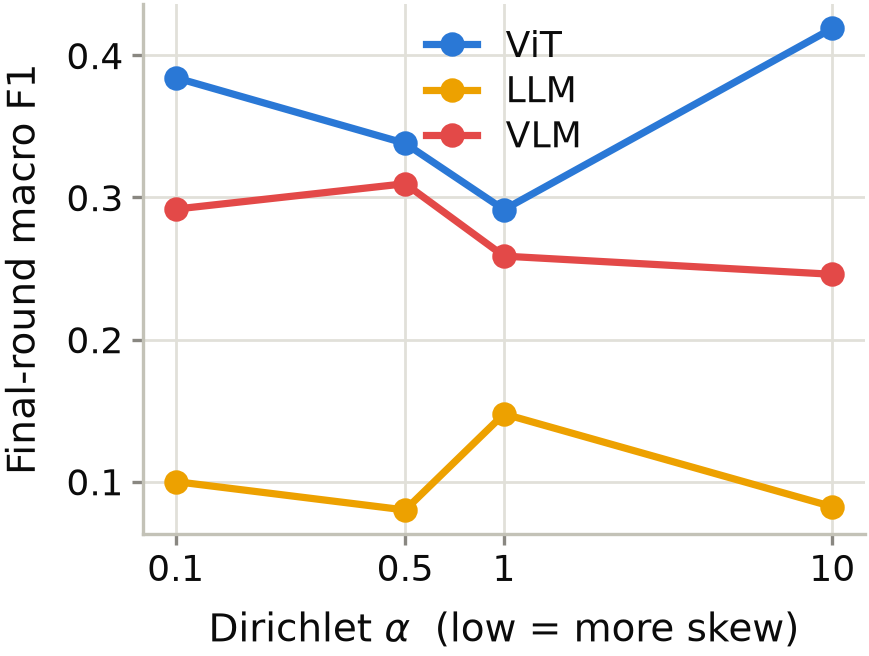
\includegraphics[width=\linewidth]{plots/panels/f10f_alpha}
    \caption{Heterogeneity $\alpha$: best at \emph{both} extremes.}
  \end{subfigure}\hfill
  \begin{subfigure}[b]{0.222\textwidth}
    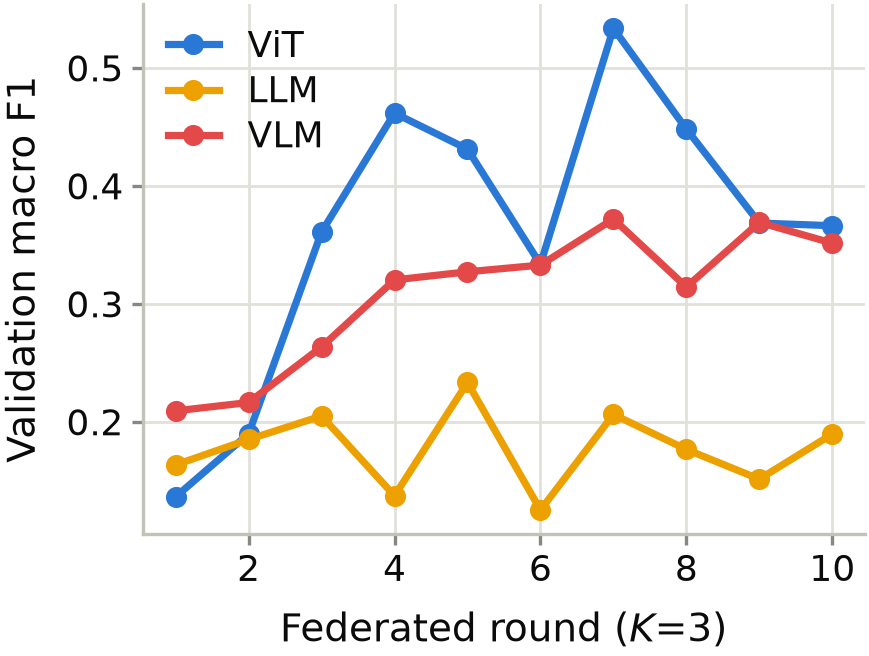
\includegraphics[width=\linewidth]{plots/panels/f10d_rounds}
    \caption{Per-round traces at the deployed $K{=}3$.}
    \label{fig:fedrounds}
  \end{subfigure}
  \caption{Federated configuration sweep (validation macro F1, compact matched-budget models). Client count (a) has no consistent direction and the curves cross; local epochs (b) is the one monotone effect; heterogeneity (c) is best at \emph{both} $\alpha$ extremes; and the per-round traces (d) never converge. None of these shapes is one a real scaling penalty produces.}
  \label{fig:fedsweep}
\end{figure*}

\begin{figure*}[!tb]
  \centering
  \begin{subfigure}[b]{0.376\textwidth}
    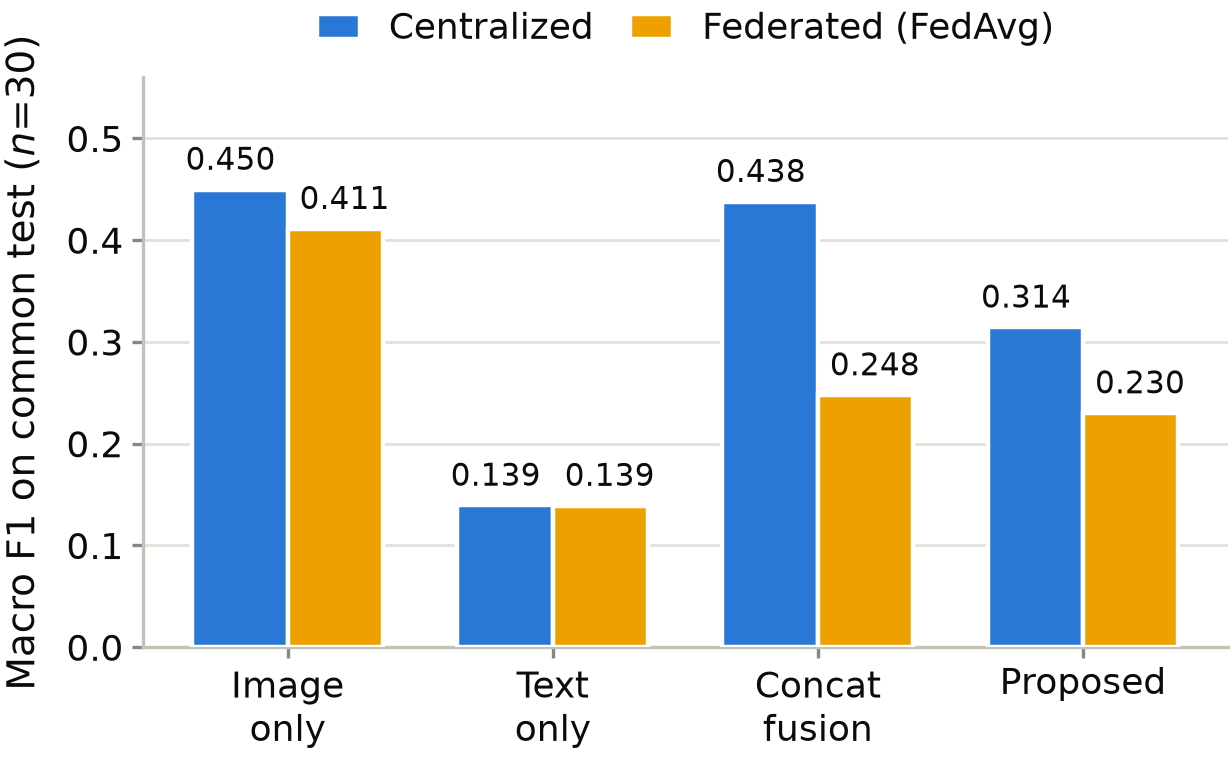
\includegraphics[width=\linewidth]{plots/panels/f11a_fedcent}
    \caption{Matched centralized vs.\ federated macro F1.}
    \label{fig:fedfour}
  \end{subfigure}\hfill
  \begin{subfigure}[b]{0.443\textwidth}
    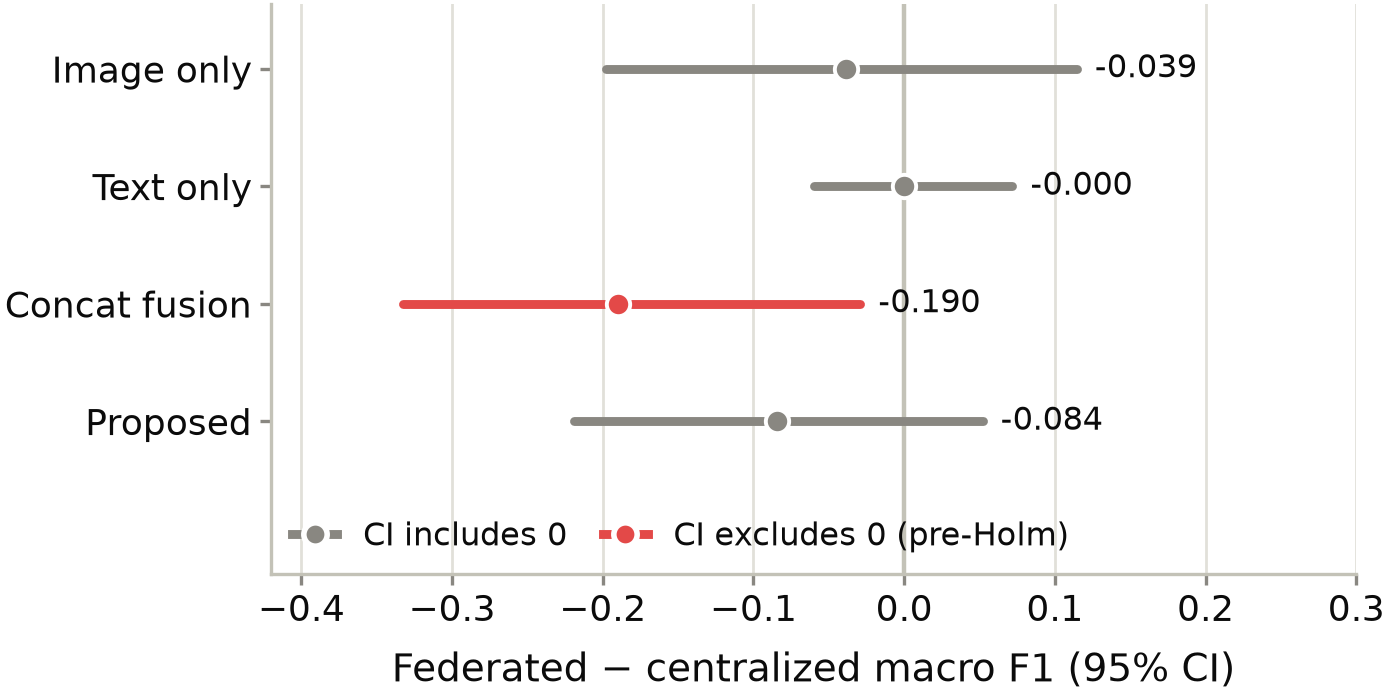
\includegraphics[width=\linewidth]{plots/panels/f11b_paired}
    \caption{Paired difference with 95\% CI.}
    \label{fig:fedpaired}
  \end{subfigure}
  \caption{Cost of federating. Pairs in (a) are matched for optimizer, pass budget, and partition, so (b) isolates the federation effect. Only concat fusion excludes zero before correction --- the condition already shown degenerate --- and after Holm correction none survives ($p{=}1.00$). Levels are matched-budget, not comparable to Table~\ref{tab:fourway}.}
  \label{fig:fedeffect}
\end{figure*}

\subsection{Why the Image Branch Contributes Nothing: Gate Collapse}
\label{sec:gatecollapse}

Two independent probes show the visual branch is inert at the deployed gate.

\textbf{Missing-modality decomposition.} Evaluating the single proposed checkpoint
through its three interfaces gives text-only 0.888, image-only 0.503, and joint
0.888 --- with byte-identical per-class F1 vectors for the text-only and joint
paths. At $w_t{=}0.70$ the text posterior dominates every test item, so no
prediction ever flips.

\textbf{Corruption sweeps} (Table~\ref{tab:robust}, Fig.~\ref{fig:robust}). The
two rows per model are near-perfect mirror images. Deleting every attended text
token leaves concat at exactly 0.511; its text branch is inert. Replacing the
image with pure noise leaves the proposed model at exactly 0.888; its image branch
is inert. \emph{Neither} model is genuinely multimodal --- they have collapsed onto
opposite modalities. The proposed model's apparent robustness to visual
corruption is not robustness; it is non-use.

\begin{table}[t]
\caption{Modality Corruption Sweep (Macro F1, $n{=}30$)}
\label{tab:robust}
\centering\footnotesize
\setlength\tabcolsep{2.6pt}
\begin{tabular}{llccccc}
\toprule
& & \multicolumn{5}{c}{\textbf{Severity}}\\
\cmidrule(lr){3-7}
\textbf{Model} & \textbf{Corruption} & 0.00 & 0.25 & 0.50 & 0.75 & 1.00\\
\midrule
\multirow{2}{*}{Concat} & Text deletion & 0.511 & 0.511 & 0.511 & 0.511 & 0.511\\
                        & Image noise   & 0.511 & 0.144 & 0.114 & 0.076 & 0.076\\
\midrule
\multirow{2}{*}{Proposed} & Text deletion & 0.888 & 0.810 & 0.680 & 0.560 & 0.434\\
                          & Image noise   & 0.888 & 0.888 & 0.888 & 0.888 & 0.888\\
\bottomrule
\end{tabular}
\end{table}

\begin{figure*}[!tb]
  \centering
  \begin{subfigure}[b]{0.452\textwidth}
    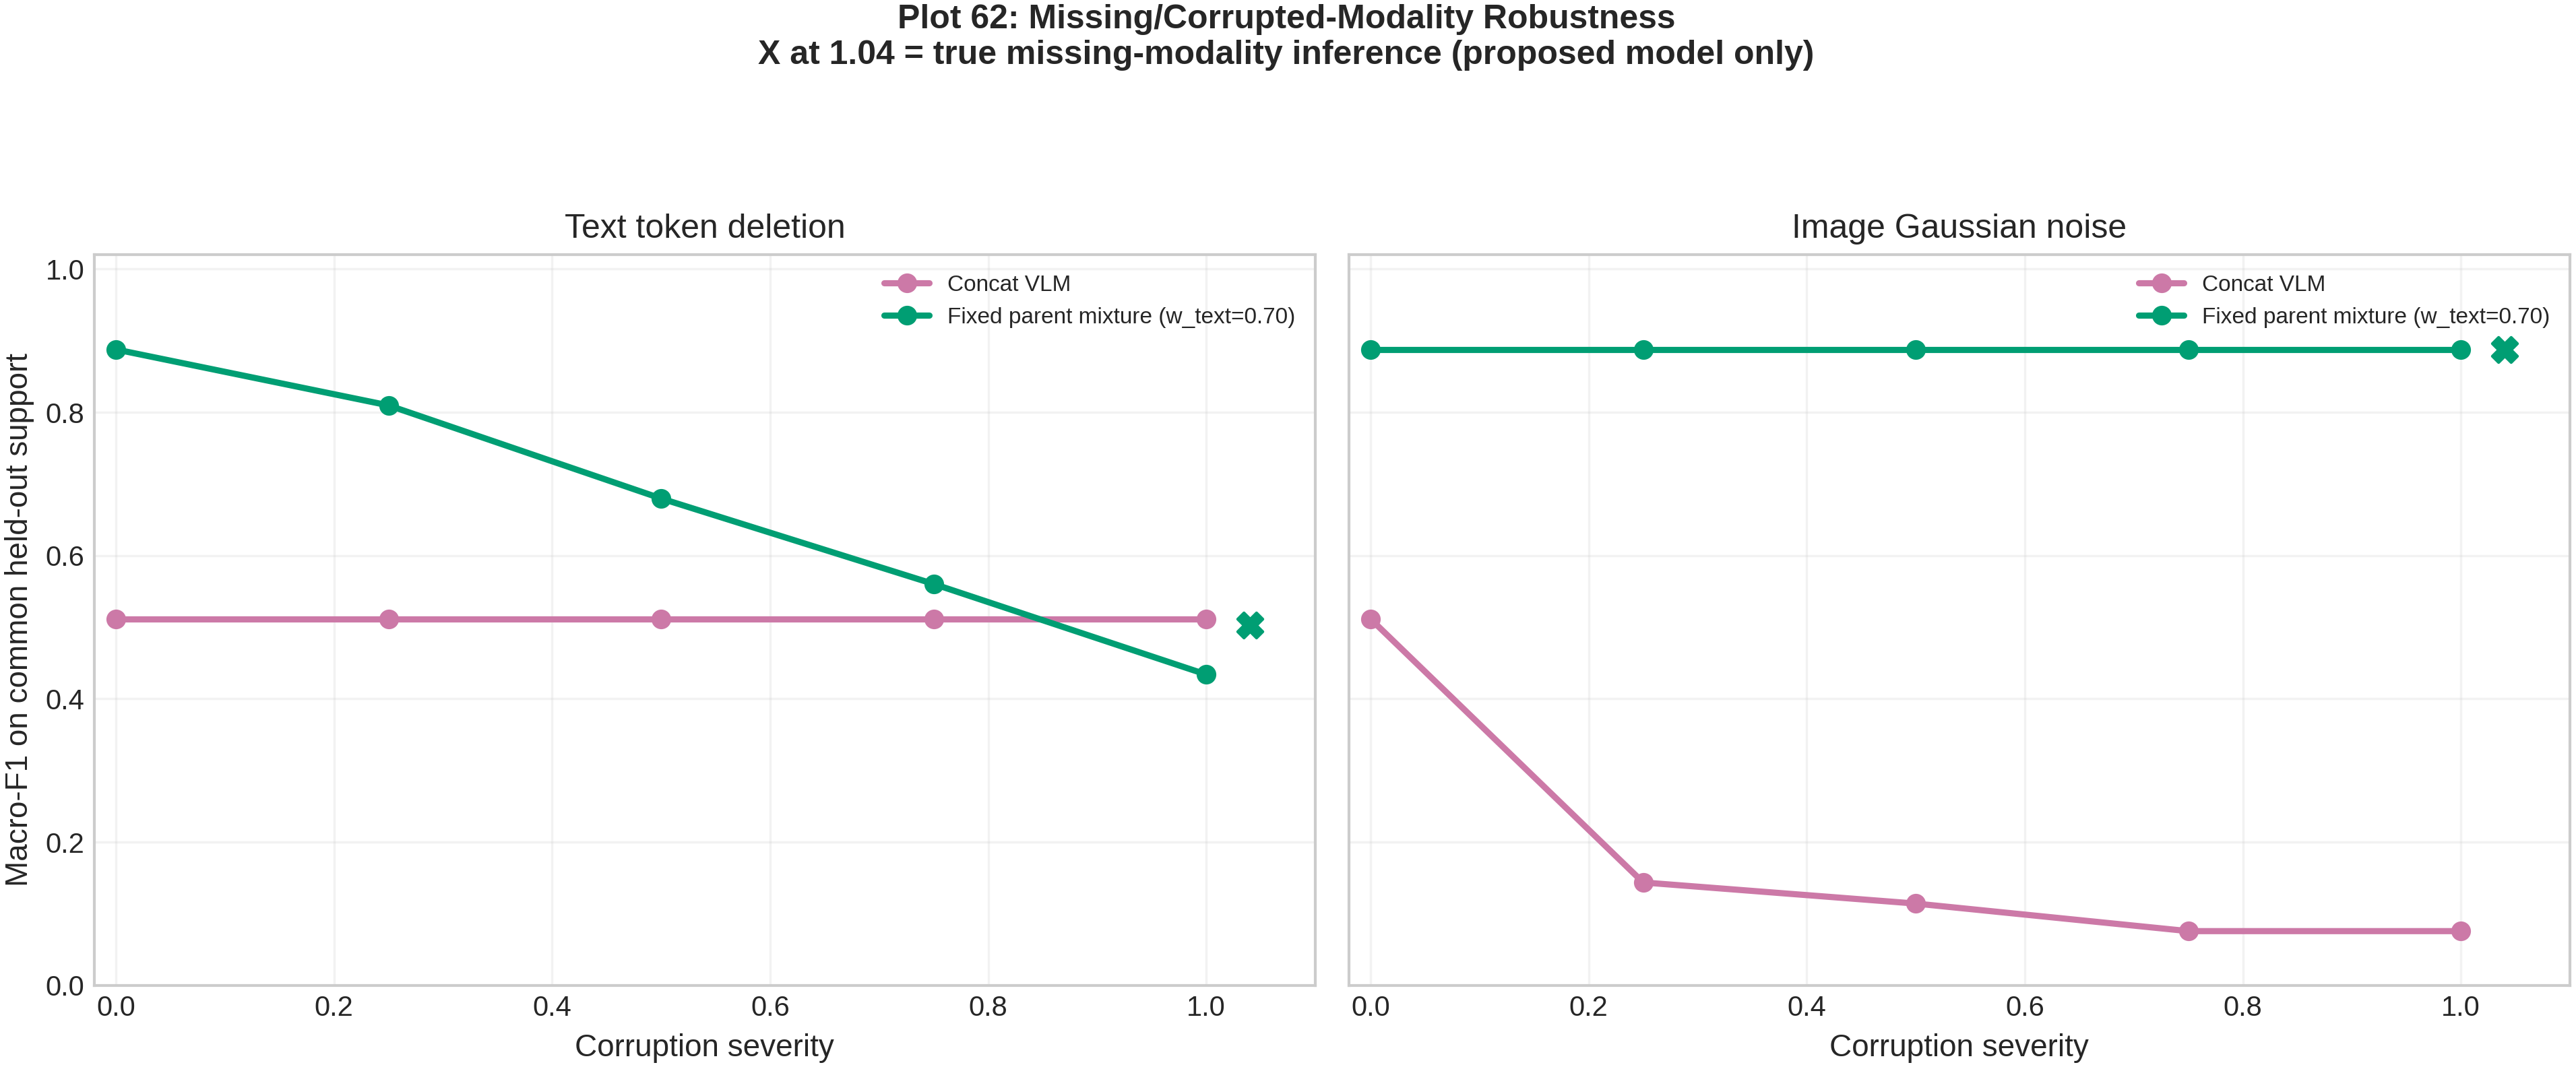
\includegraphics[width=\linewidth]{plots/plot62_modality_robustness}
    \caption{Graded single-modality corruption.}
    \label{fig:robustsweep}
  \end{subfigure}%
  \begin{subfigure}[b]{0.363\textwidth}
    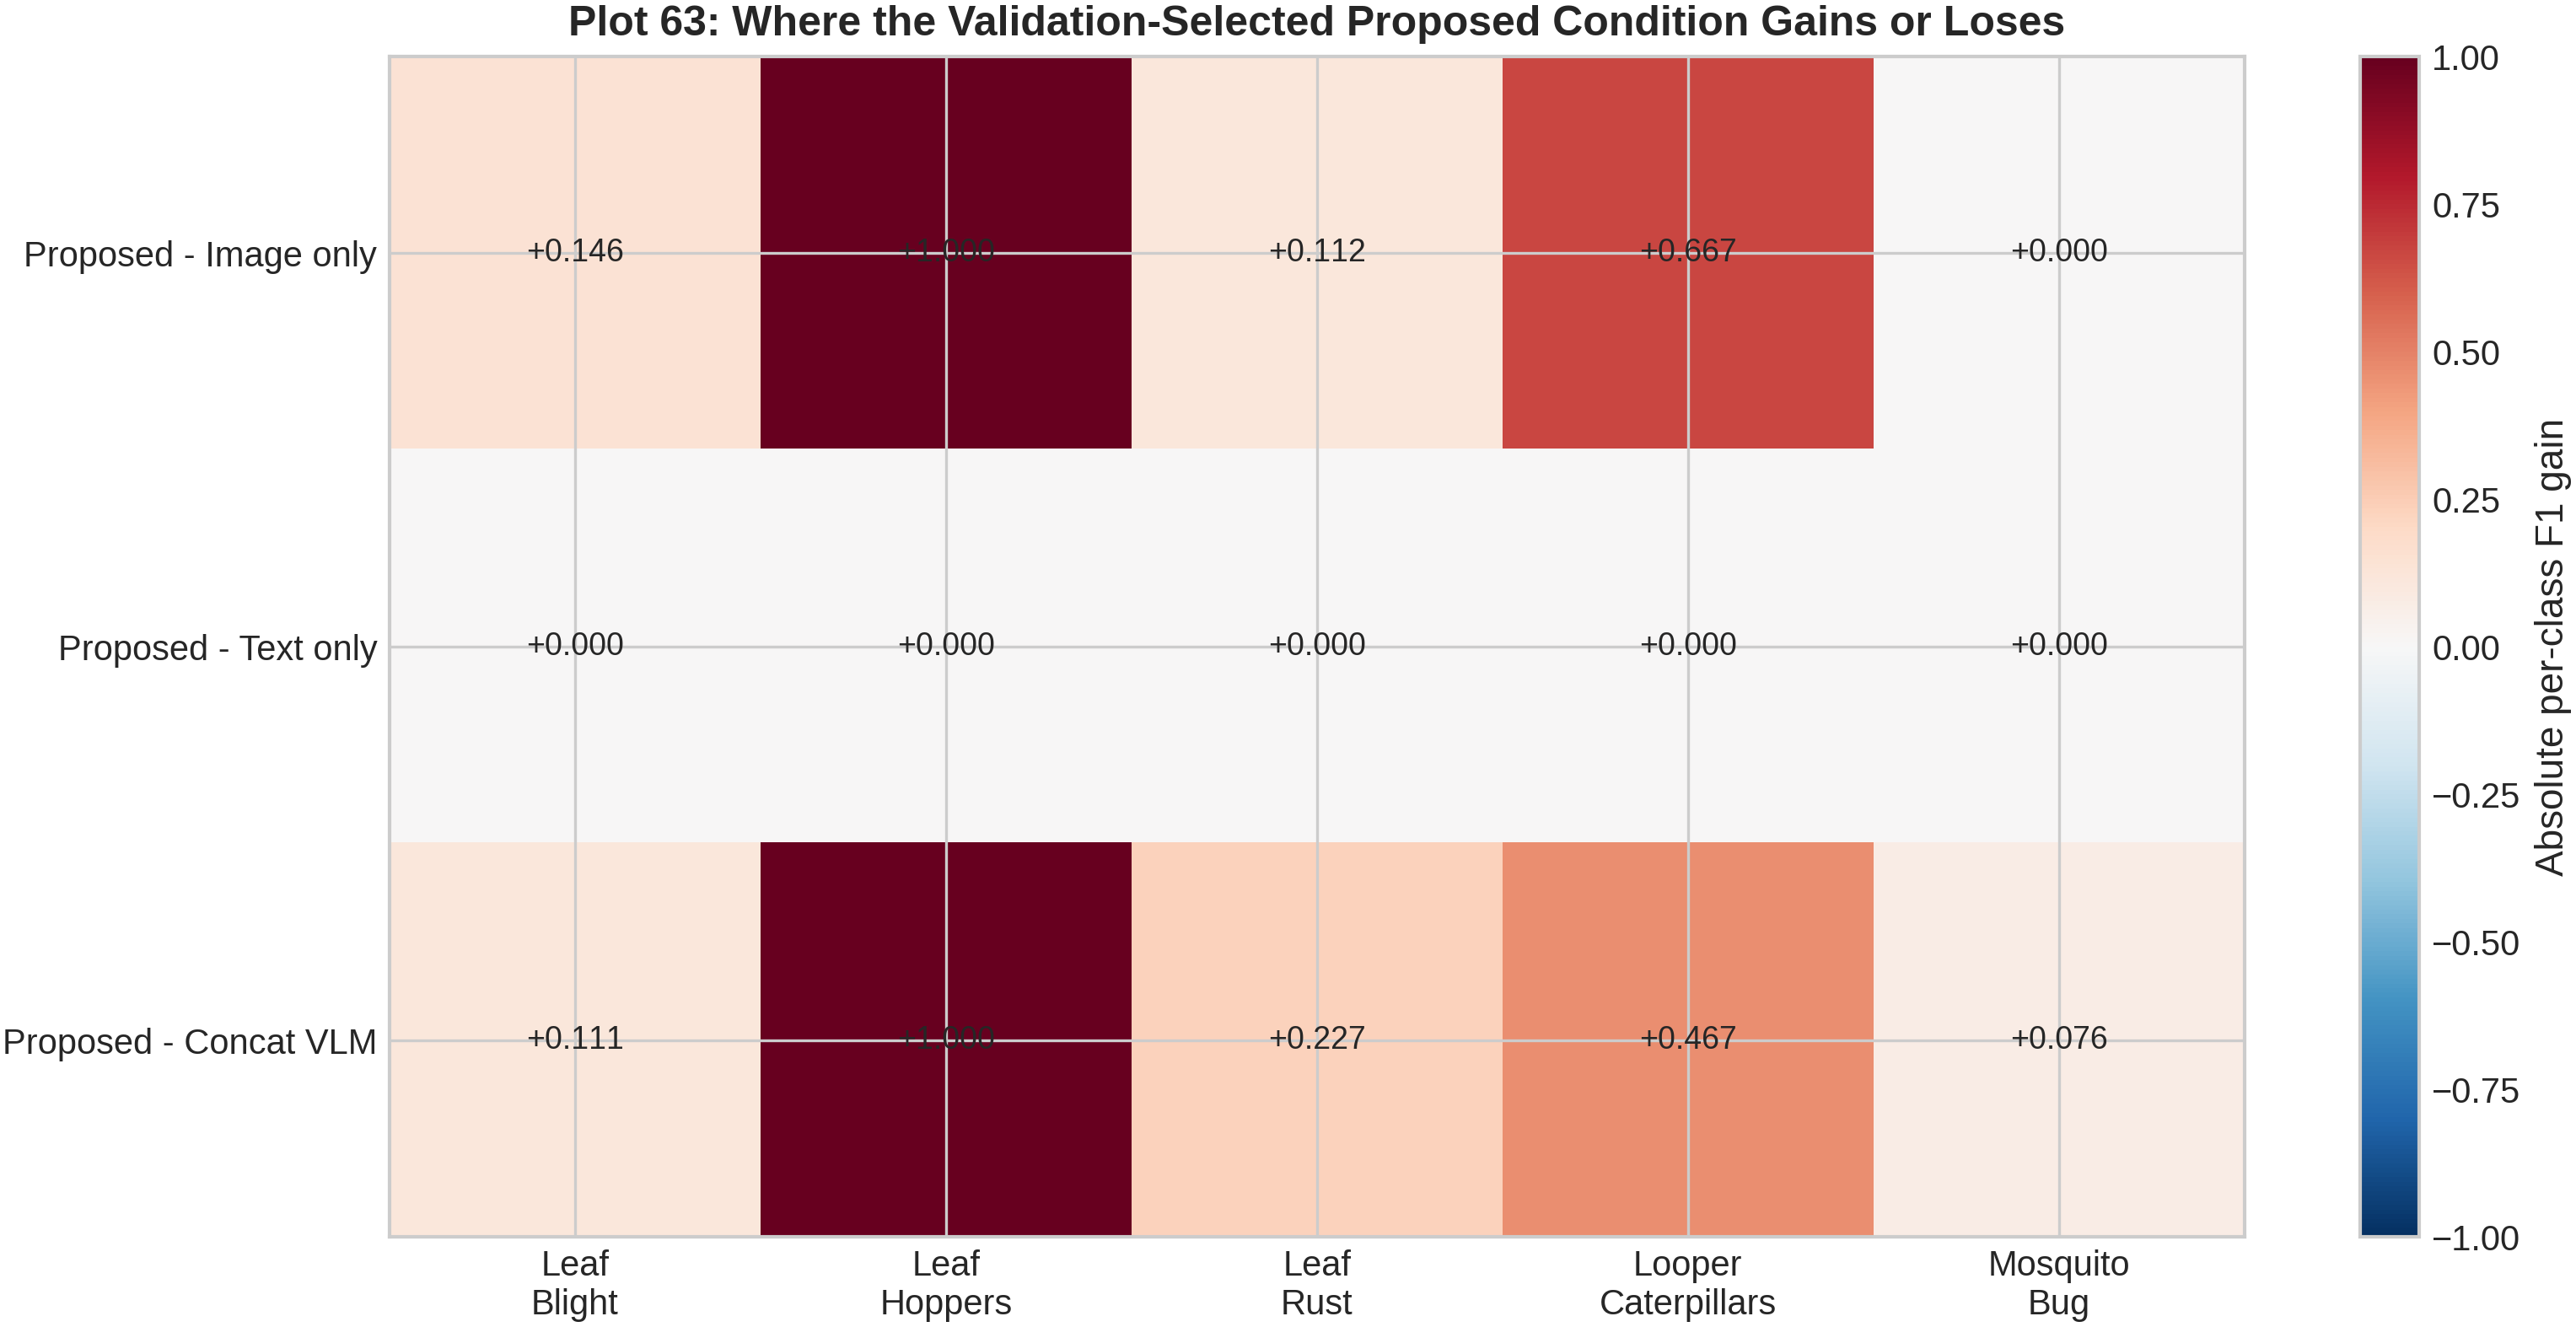
\includegraphics[width=\linewidth]{plots/plot63_per_class_modality_gain}
    \caption{Per-class gain attribution by modality.}
    \label{fig:perclassgain}
  \end{subfigure}
  \caption{Modality contribution analysis. Each model is insensitive to corruption of exactly one modality, indicating collapse onto the other rather than integration.}
  \label{fig:robust}
\end{figure*}

\subsection{Why Multimodal Accuracy Is Low: Headroom and Selection}
\label{sec:headroom}

Gate collapse explains why the image is ignored, not whether ignoring it cost
anything. Table~\ref{tab:complement} and Figure~\ref{fig:complement} decompose
the test support by which modality is correct.

\begin{table}[t]
\caption{Modality Complementarity ($n{=}30$)}
\label{tab:complement}
\centering\footnotesize
\setlength\tabcolsep{4pt}
\begin{tabular}{lcl}
\toprule
\textbf{Outcome} & \textbf{Count} & \textbf{Character}\\
\midrule
Both correct               & 17 & mosquito, rust, looper\\
Text correct, image wrong  & 9  & mostly looper, blight\\
\rowcolor{vlmred!30}
Image correct, text wrong  & 2  & blight called rust by text\\
Neither correct            & 2  & 1 blight, 1 rust\\
\midrule
\textbf{Oracle (either correct)} & \textbf{28/30} & \textbf{accuracy 0.933}\\
Text only (deployed parent)      & 26/30 & accuracy 0.867\\
\bottomrule
\end{tabular}
\end{table}

Two facts follow, and together they are the answer to why multimodal accuracy is
not higher.

\textbf{First, there was very little to win.} The modalities are genuinely
complementary but thinly and asymmetrically so: the image branch uniquely rescues
2 items --- both blight photographs the text branch called rust, exactly the
necrosis-versus-pustule ambiguity that motivates multimodal diagnosis --- while
text uniquely rescues 9. An oracle consulting whichever modality is right reaches
0.933 against the text parent's 0.867, so $+0.067$ accuracy is the ceiling on what
\emph{any} fusion rule could have won. Multimodal scores are not dramatically
above text-only because on this corpus there are only two items available.

\begin{figure*}[!tb]
\centering
\begin{subfigure}[b]{0.222\textwidth}
  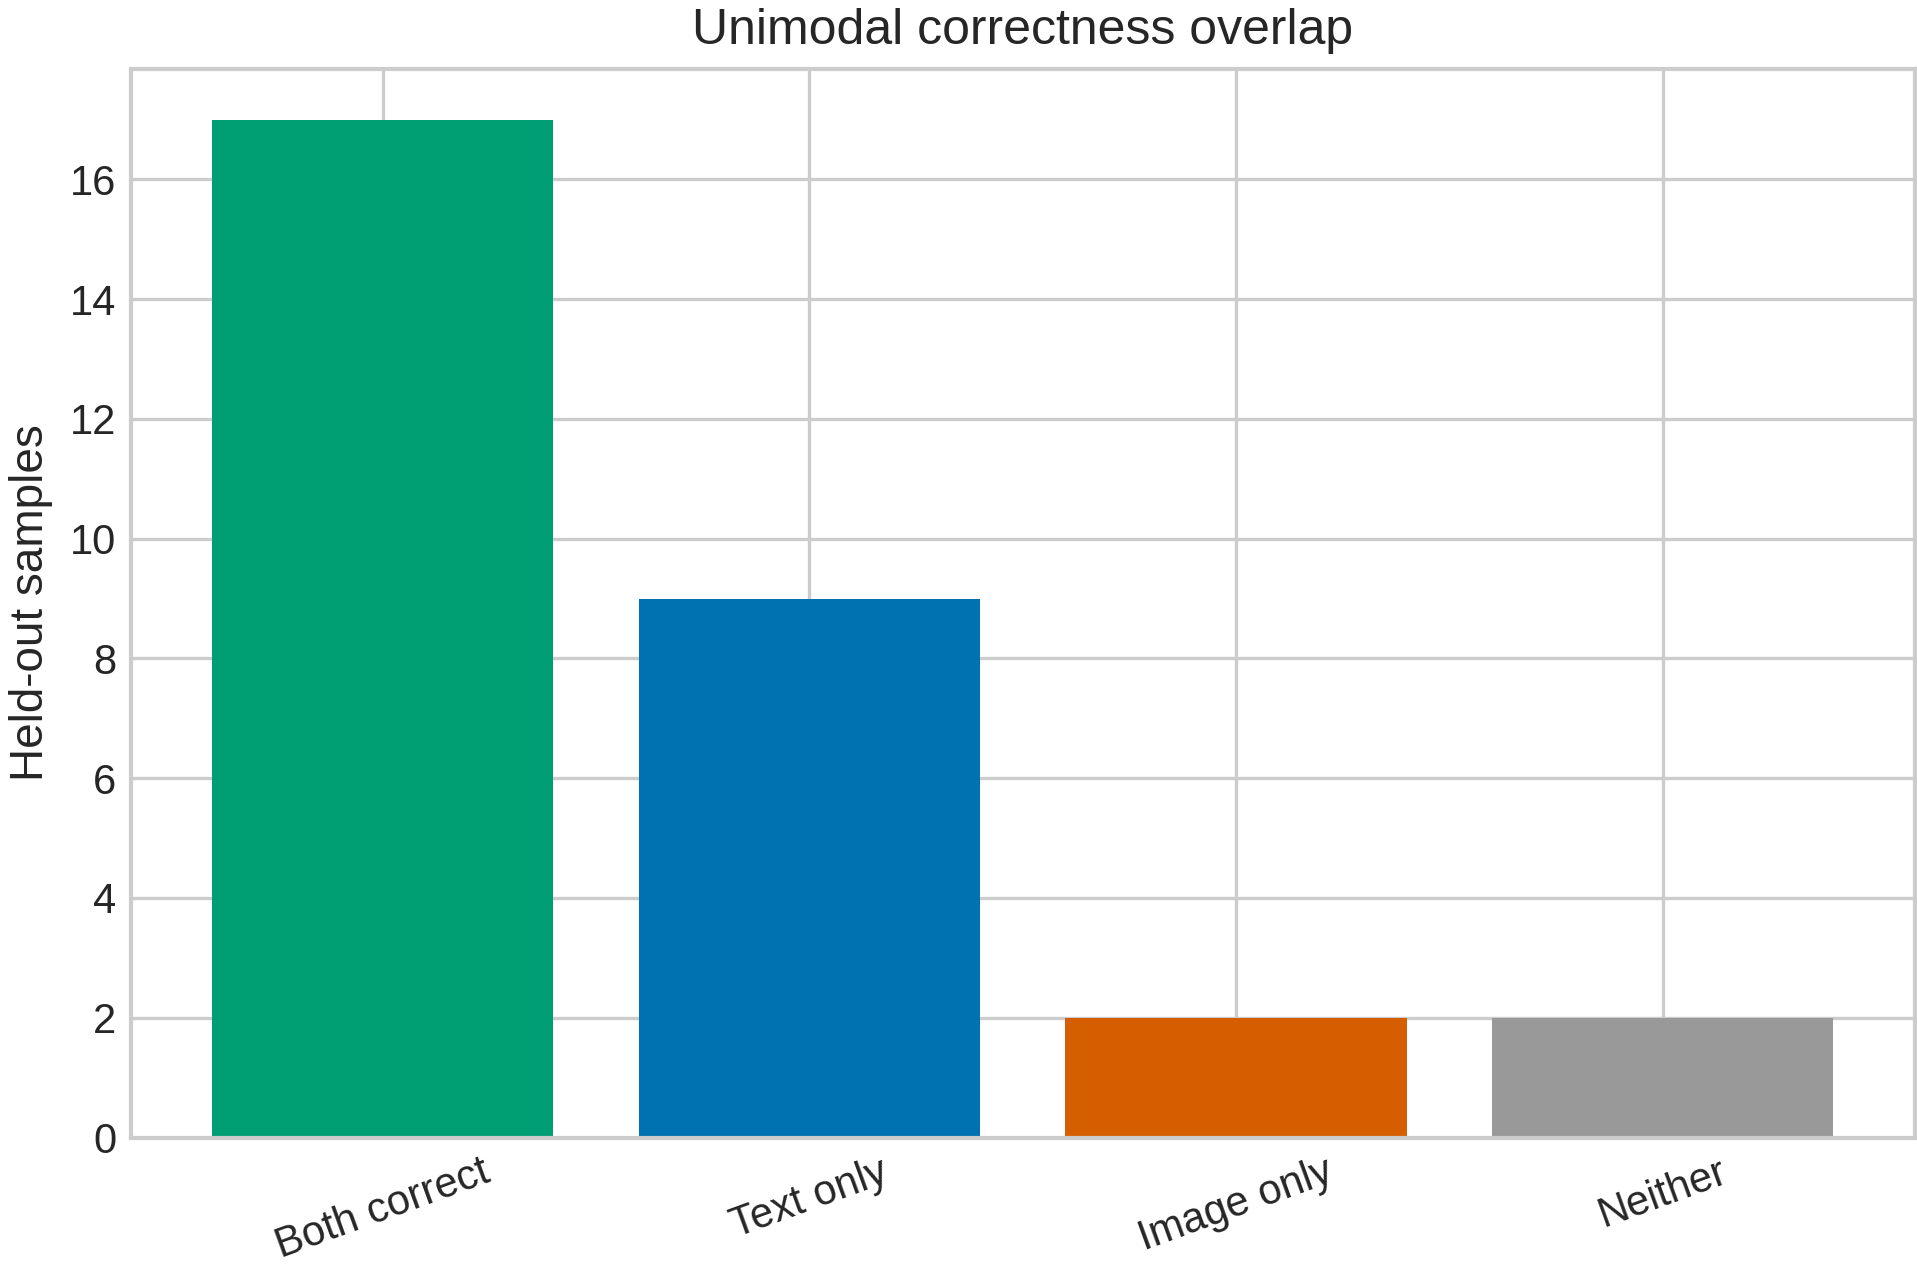
\includegraphics[width=\linewidth]{plots/panels/p60a_overlap}
  \caption{Correctness overlap: only 2 of 30 items are image-rescued, against 9 text-rescued.}
\end{subfigure}\hfill
\begin{subfigure}[b]{0.222\textwidth}
  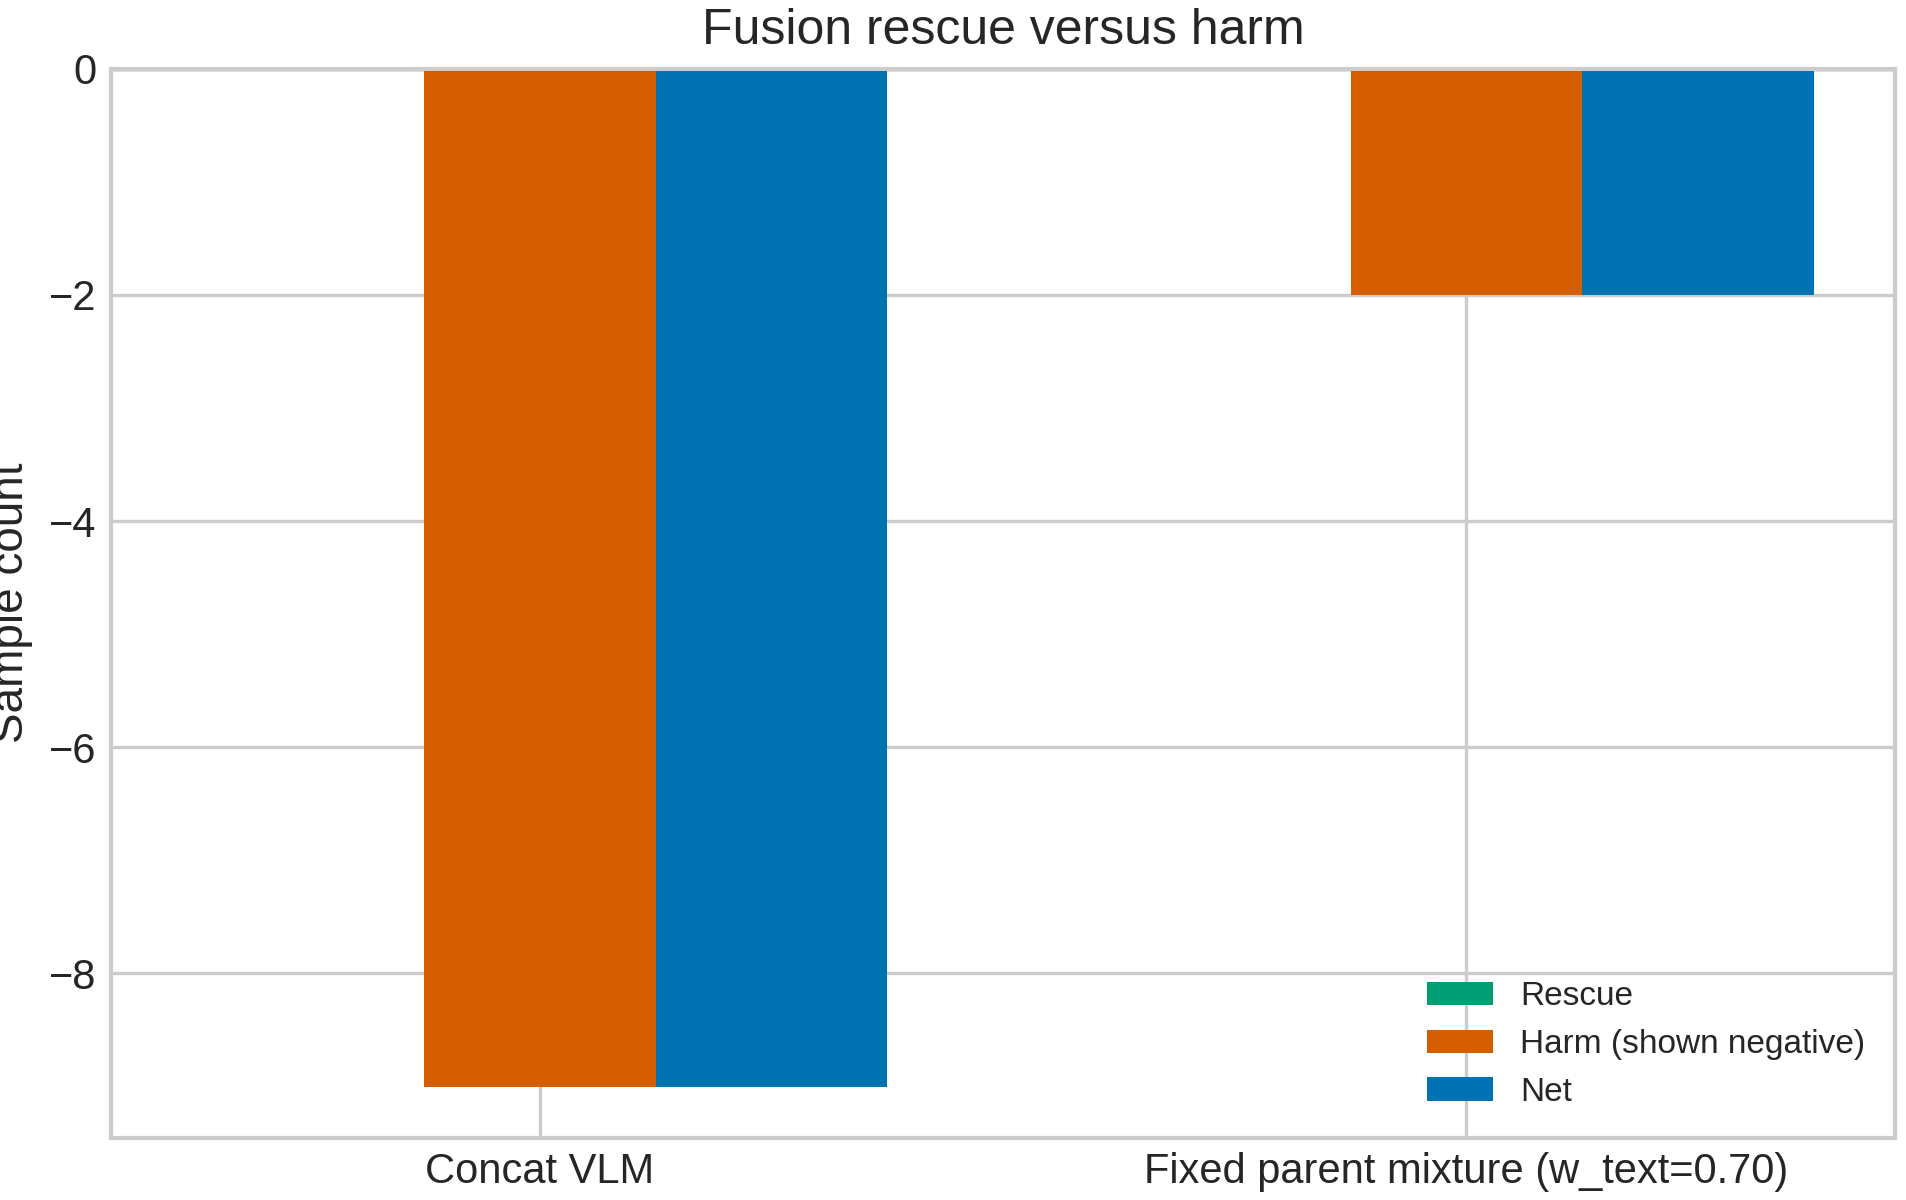
\includegraphics[width=\linewidth]{plots/panels/p60b_rescue}
  \caption{Rescue vs.\ harm: both fusion models are net-negative, concat by $-9$, the gate by $-2$.}
\end{subfigure}\hfill
\begin{subfigure}[b]{0.222\textwidth}
  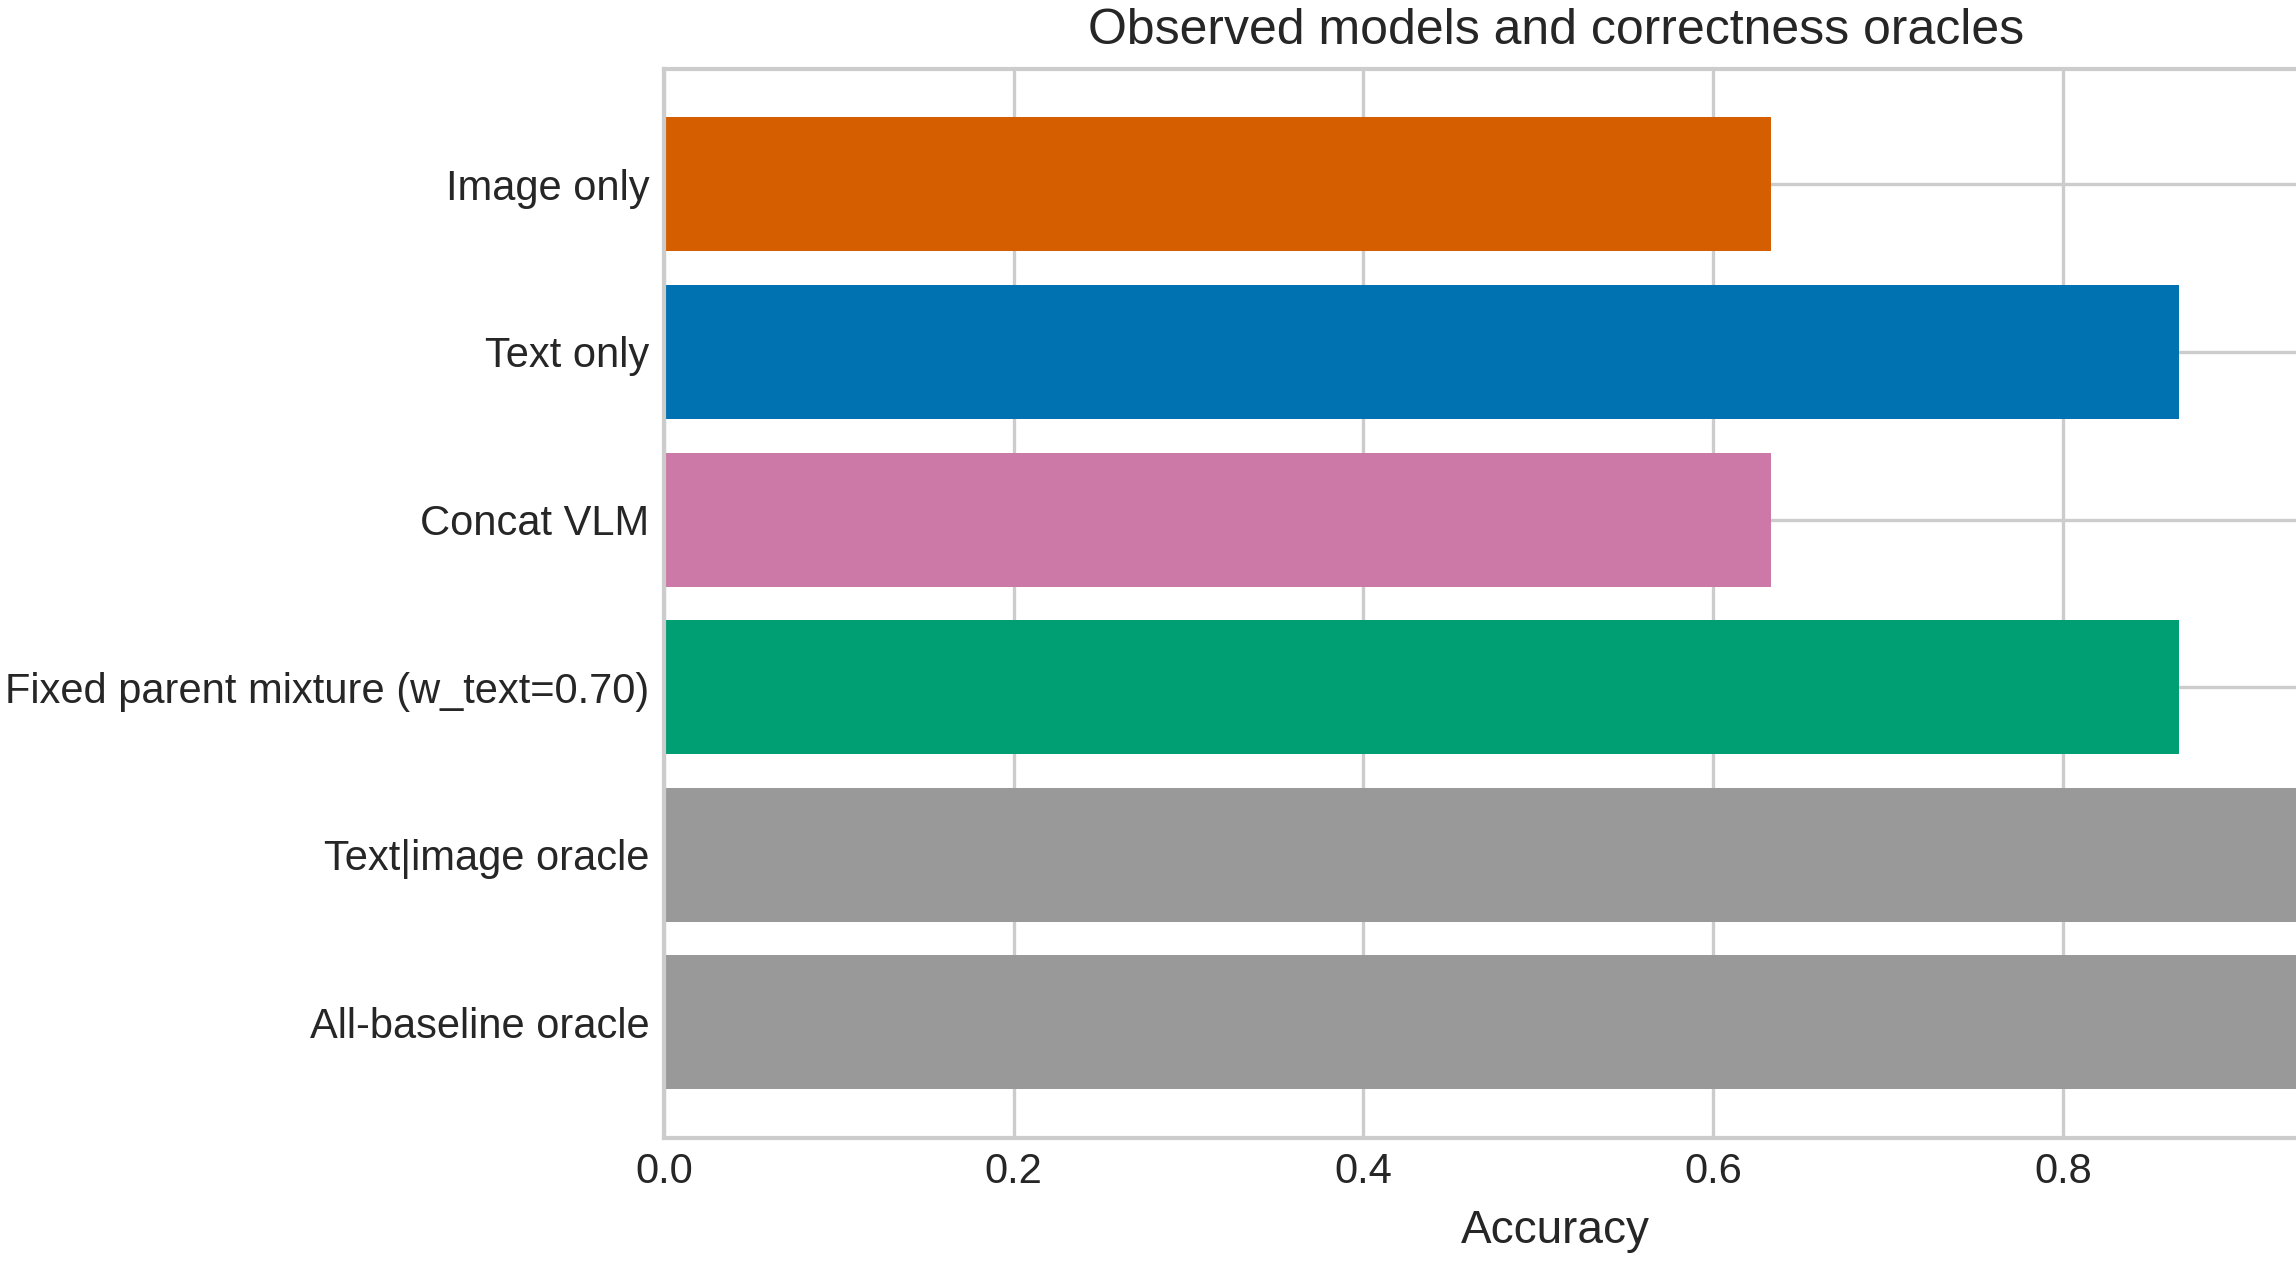
\includegraphics[width=\linewidth]{plots/panels/p60c_oracle}
  \caption{Against the oracle: text-only and the gate both 0.867, oracle 0.933 --- a 0.067 gap.}
\end{subfigure}\hfill
\begin{subfigure}[b]{0.222\textwidth}
  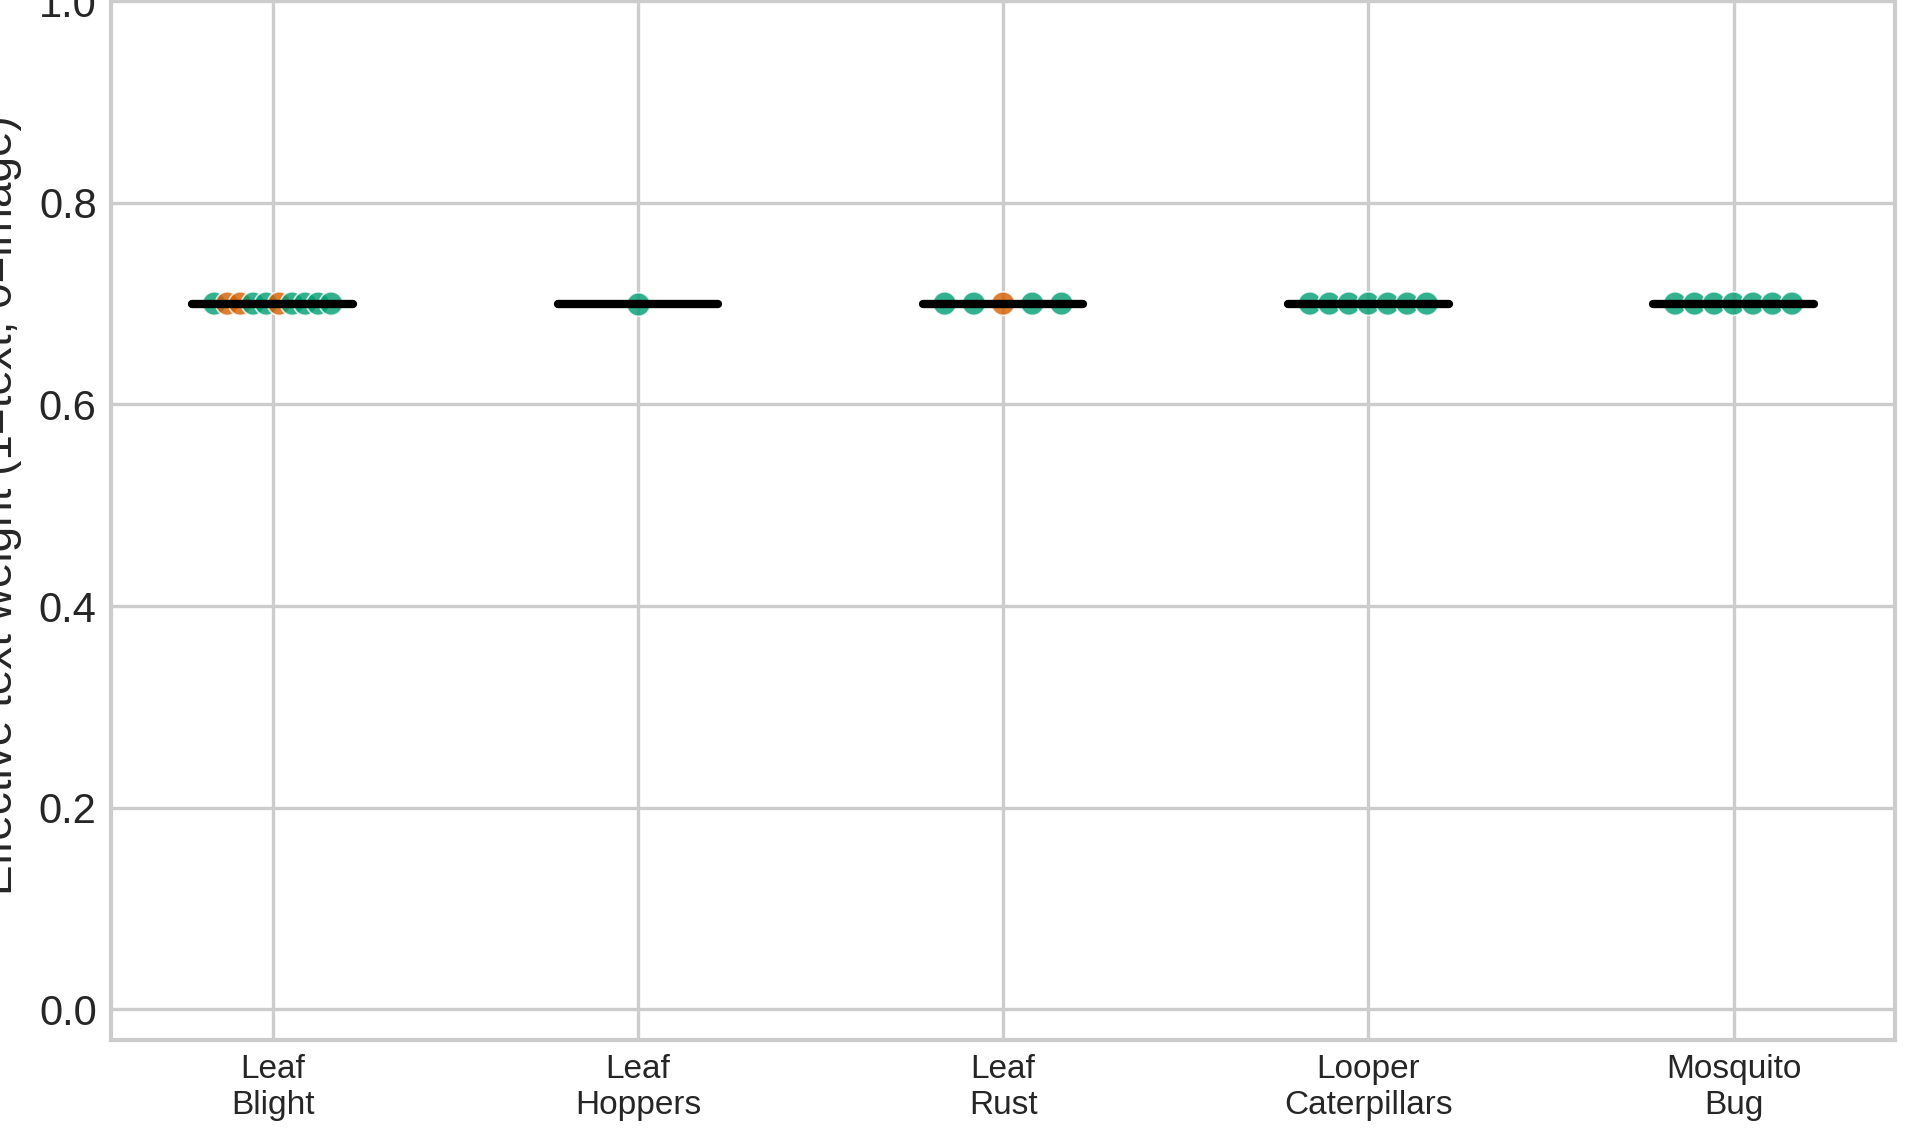
\includegraphics[width=\linewidth]{plots/panels/p60d_gate}
  \caption{Effective text weight is a flat 0.70 for every sample of every class.}
\end{subfigure}
\caption{Why multimodal accuracy is not higher. The complementarity exists (a) but is worth only two items; both fusion rules spend it and more (b); the realised accuracies leave the oracle's 0.067 unclaimed (c); and the deployed gate never adapts to any class (d), which is gate collapse made visible.}
\label{fig:complement}
\end{figure*}

\textbf{Second, the deployed gate captured none of those two, and that is a
selection failure.} Sweeping Eq.~\ref{eq:mixture} across $w_t$ on the test set
(Table~\ref{tab:wsweep}) shows a fixed mixture at $w_t\in[0.46,0.48]$ attains the
oracle exactly --- 28/30, macro F1 0.944 --- recovering both blight items while
losing nothing. The architecture was capable of extracting all available
complementarity; the deployed configuration extracted none.

\begin{table}[t]
\caption{Post-hoc mixture-weight sweep (test set, \emph{diagnostic only}). The validation column reports the nearest points of the coarser selection grid $\{0.05,0.1,0.2,\ldots,0.95\}$; the productive band was never a selection candidate.}
\label{tab:wsweep}
\centering\footnotesize
\setlength\tabcolsep{4pt}
\begin{tabular}{lccc}
\toprule
\textbf{$w_t$ range} & \textbf{Test acc.} & \textbf{Test macro F1} & \textbf{Val.\ macro}\\
\midrule
0.00--0.05 (vision end) & 0.633 & 0.503 & 0.742\\
0.36--0.45              & 0.900 & 0.911 & 0.971\\
\rowcolor{vitgreen!35}
0.46--0.48              & \textbf{0.933} & \textbf{0.944} & 0.971\\
\rowcolor{vlmred!30}
0.70 (deployed)         & 0.867 & 0.888 & \textbf{1.000}\\
1.00 (text end)         & 0.867 & 0.888 & 1.000\\
\bottomrule
\end{tabular}
\end{table}

\textbf{The shaded green row is not a result.} It was found by sweeping on test,
the exact protocol violation this paper is organised against, and we would reject
it from any other submission. It is a \emph{diagnostic}, and it localises the
failure sharply: the productive window is \textbf{0.03 wide}, so a grid over
$[0.05,0.95]$ steps straight over it. Worse, validation did not merely miss the
window --- it \textbf{ranked it below the dead zone}. Every evaluated weight at or
above 0.6 saturates at 1.000 validation macro F1, while the grid points bracketing
the productive band both score 0.971. Validation was actively anti-correlated with
test performance across the region that mattered, and the tie-break (nearest the
initialised gate prior) then selected 0.70.

The root cause is the 30-pair validation support. A criterion that saturates
cannot rank, and a 0.03-wide optimum cannot be resolved where one flipped
prediction moves the score by 0.033. This also means the $[0.46,0.48]$ window is
itself a two-item effect and is very likely overfit to this split --- which argues
for a larger evaluation set, not for deploying $w_t{=}0.47$.

\subsection{Federated Training}
\label{sec:fedres}

\textbf{The federated question has an encouraging answer.} All four paired
differences in Table~\ref{tab:fed} are negative but small, and none survives Holm
correction ($p{=}1.0$). Only concat has an interval excluding zero before
correction, and it is already degenerate. Under a matched 24-pass budget and a
skewed three-client partition, exchanging only model updates costs little or
nothing measurable.

\textbf{Absolute levels here are not comparable to Table~\ref{tab:fourway}.} The
federated arm retrains compact architectures (4.97M image, 11.1M text) from shared
initialization under a fixed budget rather than fine-tuning the large pretrained
parents; text-only drops to 0.139 because the matched-budget model collapses to
two classes. Each $\Delta$ compares like with like, but the absolute values
describe the matched-budget regime.

\textbf{The sweep is exploratory and underpowered}
(Fig.~\ref{fig:fedsweep}). Only
local epochs shows a consistent effect: $E{=}1\to5$ raises macro F1 monotonically
for ViT (0.182$\to$0.332) and VLM (0.172$\to$0.337), at roughly linear round-time
cost (1.8\,s to 13.2\,s per round). Client count has no consistent direction --- ViT and VLM degrade while LLM
improves to its maximum at $K{=}10$ --- and crossing curves on a fixed data budget
signal noise, not a scaling law. Rounds do not converge cleanly: traces oscillate
by 0.2--0.3 micro F1, and ViT at $K{=}3$ peaks at 0.633 but ends at 0.400, so
last-round reporting would understate it by 0.23. This is why every headline number
here comes from a validation-selected checkpoint. Heterogeneity is the clearest
null: ViT is best at $\alpha{=}10$ (near-IID) and second best at $\alpha{=}0.1$
(most skewed), which no monotone penalty can produce.

\begin{table}[!t]
\caption{Eligibility ledger: what this evaluation does and does not license. ``Not eligible'' means the study design cannot support the claim at all, independent of the numbers obtained.}
\label{tab:ledger}
\centering\scriptsize
\setlength\tabcolsep{2.2pt}
\renewcommand{\arraystretch}{1.05}
\begin{tabular}{@{}p{0.335\columnwidth}p{0.155\columnwidth}p{0.44\columnwidth}@{}}
\toprule
\textbf{Claim} & \textbf{Status} & \textbf{Governing evidence}\\
\midrule
\rowcolor{vitgreen!28}
Text alone beats image alone & Supported & paired $\Delta$ $+0.385$, CI $0.245$--$0.519$\\
\rowcolor{vitgreen!28}
Modalities are complementary & Supported & oracle $0.933$ vs.\ $0.867$ (2 items)\\
\rowcolor{vitgreen!28}
FedAvg $\approx$ centralized & Supported & all four $p_{\text{Holm}}{=}1.00$\\
\midrule
\rowcolor{vlmred!28}
Fusion beats the stronger parent & Not supported & gain $0.000$; \emph{zero} discordant pairs\\
\rowcolor{vlmred!28}
Deployed gate exploits it & Not supported & $w_t{=}0.70$ lies outside $[0.46,0.48]$\\
\rowcolor{vlmred!28}
Accuracy target $\geq 0.90$ & Not met & $0.867$; Wilson lower bound $0.703$\\
\midrule
\rowcolor{smallgray!45}
Verified disease semantics & Not eligible & taxonomy filename-unverified\\
\rowcolor{smallgray!45}
Gain on co-observed pairs & Not eligible & pairing is label-aligned proxy only\\
\rowcolor{smallgray!45}
Advisory retrieval quality & Not evaluated & retrieval corpus empty in this run\\
\bottomrule
\end{tabular}
\end{table}

\subsection{Threats to Validity}
\label{sec:limits}

\textbf{Test support} is 30 pairs; Wilson interval half-widths span 0.13--0.15 and no
pairwise comparison survives Holm correction --- directions are supported,
significance is not. \textbf{Uncertainty} is conditional on one checkpoint per
condition; we ran no seed replicates, so training-stochasticity variance is
unmeasured. \textbf{Taxonomy} is filename-unverified, so results are five-way
group discrimination, not verified disease semantics. \textbf{Text provenance} is
undeclared, making text scores an unlinked benchmark. \textbf{Pairing} is
label-aligned proxy, not co-observation --- in our judgement the leading reason the
image adds only 2 items, since class-generic text leaves little for the image to
disambiguate. \textbf{Federation} is simulated label skew, not cross-estate domain
shift. \textbf{Leaf-hoppers} has 8 photographs total (6 train, 1 test); its
per-class F1 of 1.000 rests on one item with a Wilson recall interval of
0.207--1.000 and should be read as no evidence. \textbf{The advisory module} is
unevaluated.

%% ─────────────────────────────────────────────────────────────────────────────
\fi
\section{Conclusion}
\label{sec:conc}

On 371 linked crops, validation retains LEAF, the ResNet--compact-Transformer
router; the ViT--DistilBERT candidate's 2-crop test edge is non-significant
($p=0.82$), and only vision-encoder capacity clears the 33-run seed-noise
floor. FedAvg retains 84--94\% of the 0.6919 initialization over 2--8 simulated
clients. Fused federated training absorbs severe label skew and 70\% client
dropout (0.741--0.776 macro F1) but not staleness or poisoning: 30\%
sign-flipping clients cut it from 0.772 to 0.123, and coordinate-wise median
recovers only part of that. In the matched suite FedAvg averages 0.510/0.492
at $\alpha=0.1/1$, warm start no longer helps, and updates cost
18.9--67.2\,MiB; no E3 arm collapses, so the stack is not claimed necessary.
FarmFederate demonstrates a mobile path from photo and symptom capture to
results and advisory follow-up, with simulated monitoring views kept separate.
Multi-estate, co-observed evaluation and a measured farmer-facing deployment
remain required.

%% ─────────────────────────────────────────────────────────────────────────────
%%TRIM-BEGIN%% restore by deleting this line and the matching TRIM-END
\iffalse
\begin{figure*}[!htbp]
\centering
\begin{subfigure}[b]{0.2358\textwidth}
  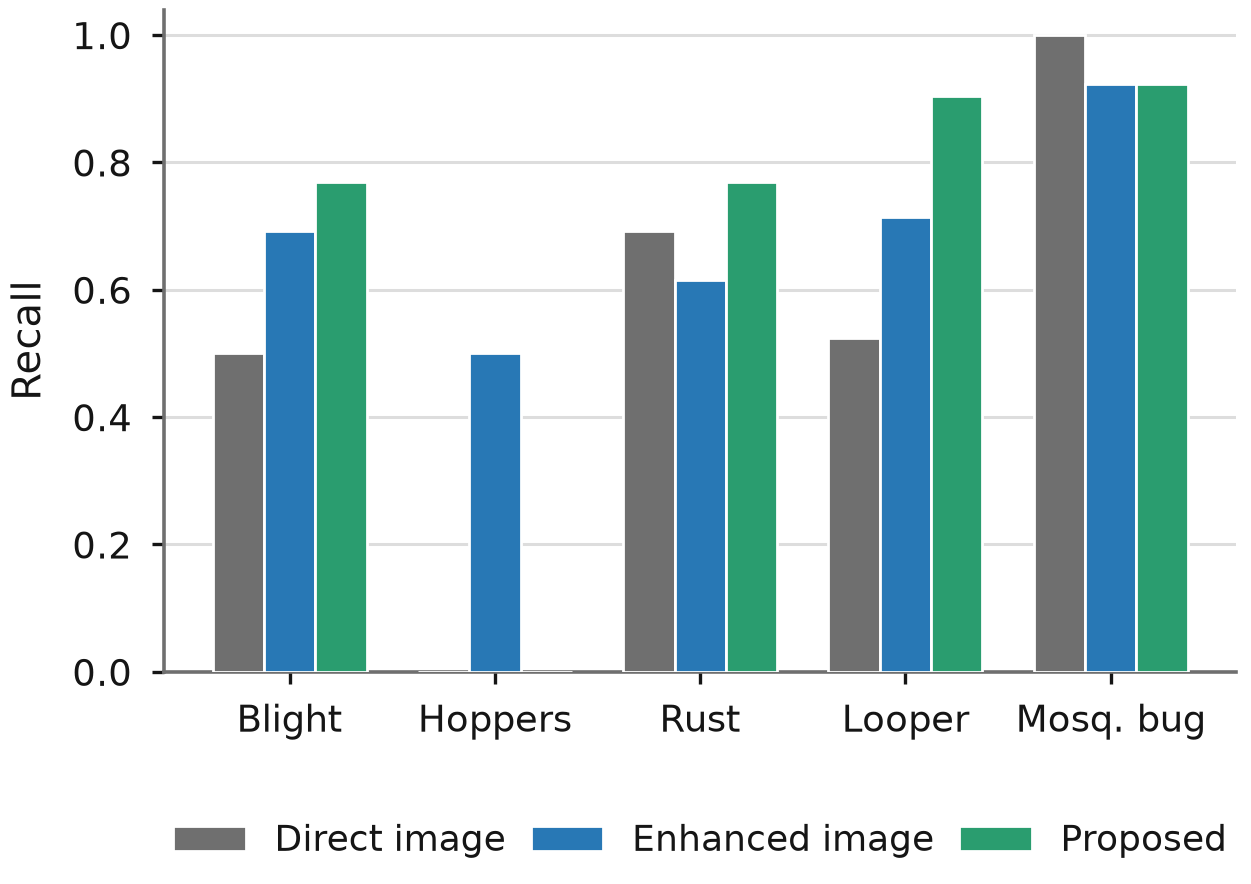
\includegraphics[width=\linewidth]{plots/plot70_classwise_recall}
  \caption{Per-class recall for the three inference paths.}
\end{subfigure}\hfill
\begin{subfigure}[b]{0.2358\textwidth}
  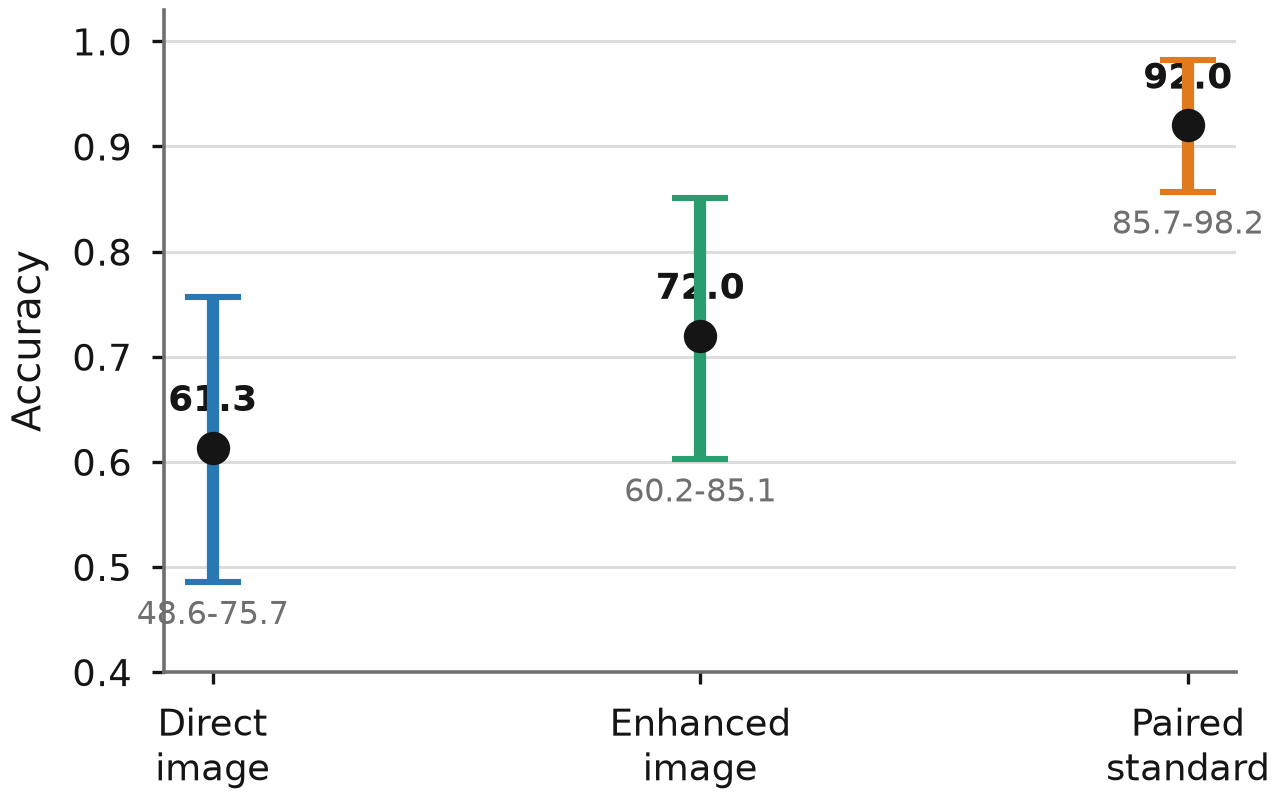
\includegraphics[width=\linewidth]{plots/plot72_source_bootstrap_accuracy}
  \caption{Source-group bootstrap accuracy intervals.}
\end{subfigure}\hfill
\begin{subfigure}[b]{0.2180\textwidth}
  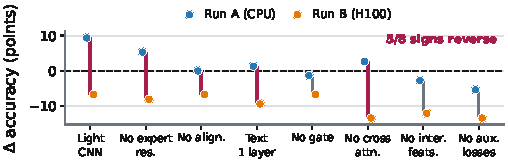
\includegraphics[width=\linewidth]{plots/plot81_architecture_effect_strip}
  \caption{Paired CPU/H100 component effects.}
  \label{fig:architecture_stability}
\end{subfigure}\hfill
\begin{subfigure}[b]{0.1379\textwidth}
  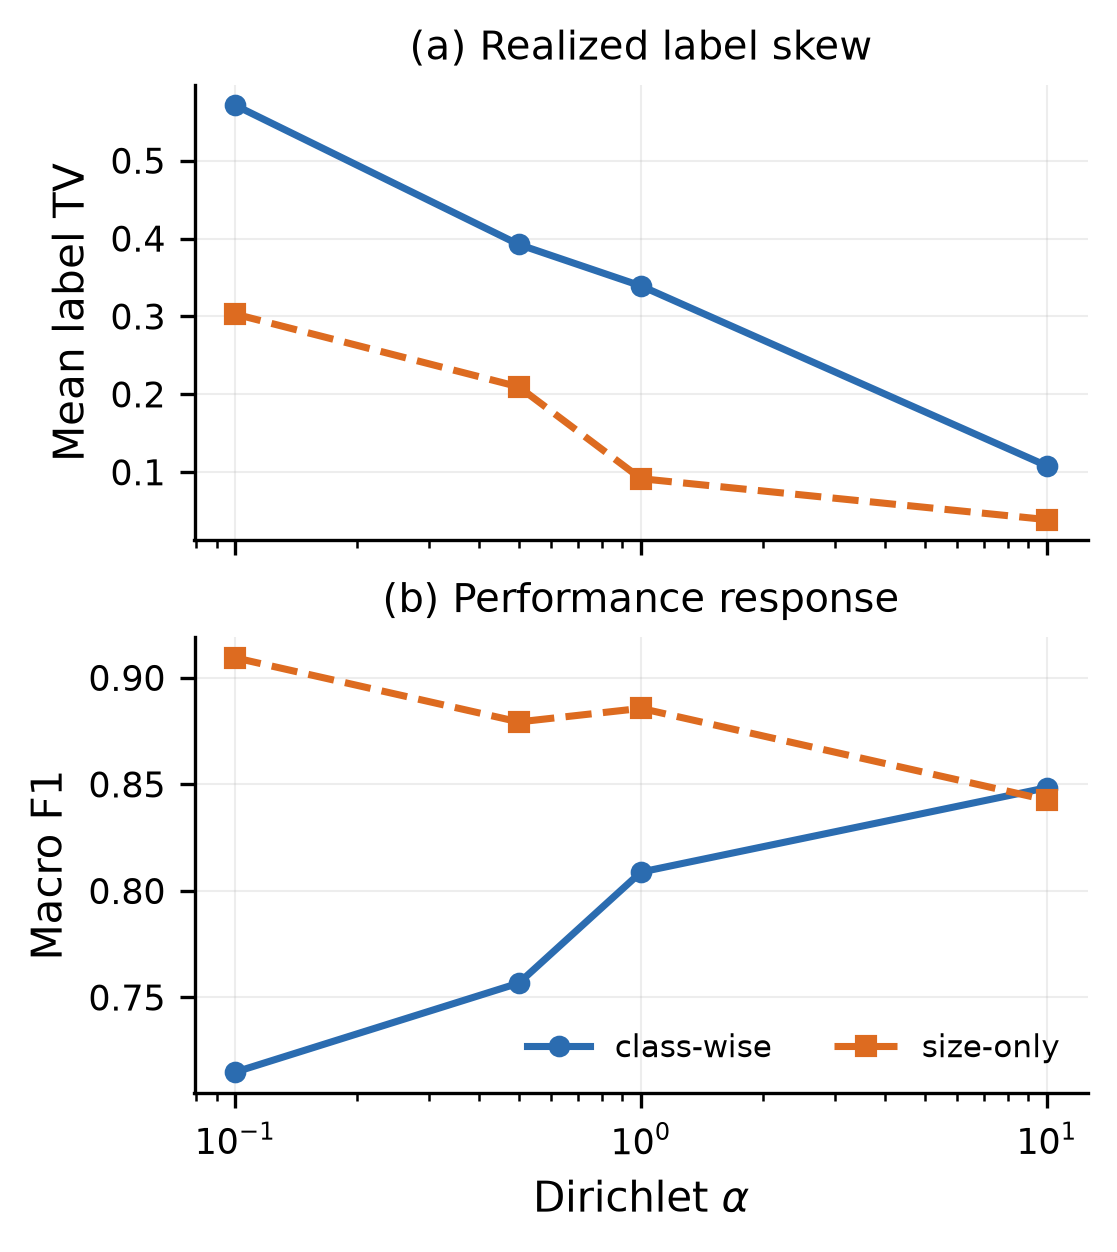
\includegraphics[width=\linewidth]{plots/plot84_alpha_split_vertical}
  \caption{Partition audit.}
  \label{fig:alpha_split_audit}
\end{subfigure}
\caption{Class-level gains, uncertainty, component stability, and partition
audit on the locked 75-crop test. Intervals in (b) resample 38 source
photographs and do not measure estate shift. In (c) red connectors cross zero
and five of eight signs reverse, so single-run deltas are not ranked. In (d) the
legacy size-only splitter stays comparatively IID.}
\label{fig:class_uncertainty}
\end{figure*}
\fi
%%TRIM-END%%

%% All floats are placed before this point; references remain the final section.
\FloatBarrier
\bibliographystyle{IEEEtran}
\let\oldbibliography\thebibliography
\renewcommand{\thebibliography}[1]{%
  \oldbibliography{#1}%
  \setlength{\itemsep}{-0.3pt}%
  \setlength{\parskip}{0pt}%
  \setlength{\topsep}{0pt}%
  \setlength{\parsep}{0pt}%
}
\begin{thebibliography}{99}
\fontsize{7}{7.3}\selectfont
\setlength{\itemsep}{-0.45pt}
\setlength{\parskip}{0pt}
\setlength{\parsep}{0pt}

\bibitem{Yang2025WaveLite}
J.~Yang, G.~Xu, M.~Yang, and Z.~Lin, ``Lightweight wavelet-{CNN} tea leaf disease
detection,'' \emph{PLOS ONE}, vol.~20, no.~5, art.~e0323322, 2025.

\bibitem{Hu2024CropProtection}
Y.~Hu, J.~Tang, and J.~Yang, ``Introducing artificial intelligence technology to
plant disease management for sustainable agriculture,'' \emph{Crop Protection},
vol.~184, art.~106764, 2024.

\bibitem{He2016ResNet}
K.~He, X.~Zhang, S.~Ren, and J.~Sun, ``Deep residual learning for image
recognition,'' in \emph{Proc.\ IEEE Conf.\ Comput.\ Vis.\ Pattern Recognit.},
2016, pp.~770--778.

\bibitem{Tahir2025FedXAI}
H.~A. Tahir, W.~Alayed, and W.~U. Hassan, ``A federated explainable {AI} framework
for smart agriculture,'' \emph{IEEE Access}, vol.~13, pp.~97567--97584, 2025.

\bibitem{Devaraj2024RuralAI}
H.~Devaraj \emph{et al.}, ``{RuralAI} in tomato farming: Integrated sensor system,
distributed computing, and hierarchical federated learning,'' \emph{IEEE Sensors
Lett.}, vol.~8, no.~5, pp.~1--4, 2024.

\bibitem{McMahan2017}
H.~B. McMahan, E.~Moore, D.~Ramage, S.~Hampson, and B.~A. y Arcas,
``Communication-efficient learning of deep networks from decentralized data,'' in
\emph{Proc.\ AISTATS}, 2017, pp.~1273--1282.

\bibitem{Dosovitskiy2021}
A.~Dosovitskiy \emph{et al.}, ``An image is worth 16x16 words: Transformers for
image recognition at scale,'' in \emph{Proc.\ ICLR}, 2021.

\bibitem{Radford2021}
A.~Radford \emph{et al.}, ``Learning transferable visual models from natural
language supervision,'' in \emph{Proc.\ ICML}, 2021, pp.~8748--8763.

\bibitem{Li2023}
J.~Li, D.~Li, S.~Savarese, and S.~Hoi, ``BLIP-2: Bootstrapping language-image
pre-training with frozen image encoders and large language models,'' in
\emph{Proc.\ ICML}, 2023.

\bibitem{Wang2025LLMICDP}
Y.~Wang \emph{et al.}, ``A large language model for multimodal identification of
crop diseases and pests,'' \emph{Scientific Reports}, vol.~15, art.~21959, 2025.

\bibitem{Li2025FedReplay}
L.~Li, J.~Li, D.~Chen, L.~Pu, H.~Yao, and Y.~Huang, ``{FedReplay}: A feature
replay assisted federated transfer learning framework for smart agriculture,''
\emph{arXiv:2511.00269}, 2025.

\bibitem{Touvron2021}
H.~Touvron, M.~Cord, M.~Douze, F.~Massa, A.~Sablayrolles, and H.~J\'{e}gou,
``Training data-efficient image transformers \& distillation through attention,''
in \emph{Proc.\ ICML}, 2021, pp.~10347--10357.

\bibitem{Liu2021Swin}
Z.~Liu \emph{et al.}, ``Swin Transformer: Hierarchical vision transformer using
shifted windows,'' in \emph{Proc.\ ICCV}, 2021, pp.~10012--10022.

\bibitem{Liu2022ConvNeXT}
Z.~Liu, H.~Mao, C.-Y. Wu, C.~Feichtenhofer, T.~Darrell, and S.~Xie, ``A ConvNet for
the 2020s,'' in \emph{Proc.\ CVPR}, 2022, pp.~11976--11986.

\bibitem{Tan2019}
M.~Tan and Q.~V. Le, ``EfficientNet: Rethinking model scaling for convolutional
neural networks,'' in \emph{Proc.\ ICML}, 2019, pp.~6105--6114.

\bibitem{Sanh2019}
V.~Sanh, L.~Debut, J.~Chaumond, and T.~Wolf, ``DistilBERT, a distilled version of
BERT,'' \emph{arXiv:1910.01108}, 2019.

\bibitem{Reimers2019}
N.~Reimers and I.~Gurevych, ``Sentence-BERT: Sentence embeddings using Siamese
BERT-networks,'' in \emph{Proc.\ EMNLP}, 2019, pp.~3982--3992.

\bibitem{Garg2025Multimodal}
P.~Garg, A.~Mishra, R.~Raja, A.~Kumar, M.~V. Joshi, and V.~S. Palaparthy,
``Multimodal data fusion by integrating IoT-enabled sensors and images for
Jamun crop disease detection with machine learning,'' \emph{IEEE Trans.\
AgriFood Electron.}, vol.~3, no.~2, pp.~582--590, 2025, doi:
10.1109/TAFE.2025.3585065.

\bibitem{Pandey2021TeaFungal}
A.~K. Pandey, G.~D. Sinniah, A.~Babu, and A.~Tanti, ``How the global tea
industry copes with fungal diseases---Challenges and opportunities,''
\emph{Plant Disease}, vol.~105, no.~7, pp.~1868--1879, 2021.

\bibitem{Dembani2025FLPrivacy}
R.~Dembani, I.~Karvelas, N.~A. Akbar, S.~Rizou, D.~Tegolo, and S.~Fountas,
``Agricultural data privacy and federated learning: A review of challenges
and opportunities,'' \emph{Comput.~Electron.~Agric.}, vol.~232,
art.~110048, 2025.

\end{thebibliography}

\end{document}
